%Execuation Instruction: (1) Bib (2) PdfLatex (3) Viewpdf

%\documentclass[handout]{beamer}
\documentclass[aspectratio=169,handout]{beamer}
\usetheme[pageofpages=of,% String used between the current page and the
                         % total page count.
          bullet=square,% Use circles instead of squares/circle for bullets.
          titleline=true,% Show a line below the frame title.
          alternativetitlepage=true,% Use the fancy title page.
          titlepagelogo=iitlogogray,% Logo for the first page.
          %watermark=iit_logoPNG,% Watermark used in every page.
          watermarkheight=100px,% Height of the watermark.
          watermarkheightmult=4,% The watermark image is 4 times bigger
                                % than watermarkheight.
]{Torino}
\usepackage{graphicx}
\graphicspath{{./Figures/}}
\definecolor{chameleongreen5}{rgb}{0.04, 0.07725, 0.18667}
\setbeamercolor{section in head/foot}{fg=white, bg=chameleongreen5}
\useoutertheme[]{miniframes}
\usefonttheme[onlymath]{serif}
\usepackage{url}
\usepackage{multicol}
\usepackage{etex}
\usepackage{tikz}
\usetikzlibrary{arrows, positioning, automata}
\usepackage{changepage}
\usepackage{multicol}
\usepackage{mathtools}

\usepackage{pgf,tikz,pgfplots}
%\pgfplotsset{compat=1.15}
\usepackage{mathrsfs}
\usetikzlibrary{arrows}
\usepackage{verbatim}
\usepackage{comment}

% put color to \boxed math command
\usepackage{tikz}
\newcommand*{\boxcolor}{slidecolor}
\makeatletter
\renewcommand{\boxed}[1]{\textcolor{\boxcolor}{%
\tikz[baseline={([yshift=-1ex]current bounding box.center)}] \node [rectangle, minimum width=2ex,rounded corners,draw,fill=slidecolor!25] {\normalcolor\m@th$\displaystyle#1$};}}
 \makeatother

\renewenvironment{comment}{}{}%

%\useoutertheme{theme name}
%default
%infolines
%miniframes
%smoothbars
%sidebar
%split
%shadow
%tree
%smoothtree
%\setbeamercolor{background canvas}{bg=white} 
%\usecolortheme{crane} 
%\useinnertheme{circles}






%\logo{\pgfimage[height=0.65cm]{SOAlogo.png}}
%\author{Marco Barisione}

%\title{Torino, a pretty theme for \LaTeX{} Beamer}
%\author[ITER, S`O'A Deemed to be University, BBSR]{{\textbf{Dr. Kundan Kumar}}\\ Ph.D. (IIT Kharagpur)\\~Associate Professor\\~ECE Department (Cabin - E139)}
%
%\institute{\vspace{-12pt}\\\pgfimage[height=1.5cm]{SOAlogo.png}\\Institute of Technical Education \& Research (ITER)\\S`O'A Deemed to be University, Bhubaneswar, Odisha, India-751030\\
%\copyright\ 2018 Kundan Kumar, All Rights Reserved}
%%\date{}



%\author{{\bf Kundan Kumar\inst{1}}\\ \bf (11EC91R02)}
%\institute{{Under the guidance of}\vspace{3pt} \\{\small {\bf Prof. P. K. Biswas}} \vspace{10pt}\\ Department of Electronics and Electrical Communication Engineering\\ Indian Institute of Technology Kharagpur, India}
%%\date{25 Sep 2014}
%\date{}
%\institute{Politecnico di Torino}
%\date{September 30, 2015}
\newenvironment{variableblock}[3]{%
  \setbeamercolor{block body}{#2}
  \setbeamercolor{block title}{#3}
  \begin{block}{#1}}{\end{block}}
  \DeclareGraphicsExtensions{.pdf,.png,.jpg}
\usepackage{multimedia}  % to include movies
\setbeamertemplate{bibliography item}{\insertbiblabel}  % to asign numbered labels to bibliography items
\usepackage{appendixnumberbeamer}
\definecolor{slidecolor}{rgb}{0.20706, 0.29725, 0.42667}
\definecolor{sc}{rgb}{0.20706, 0.29725, 0.42667}
\usepackage{booktabs}
\usepackage{subfigure}

%%%%%%%%%%%%%%%%%%%%%%%%%%%%%%%%%%%%%%%%%%%%%%%%%%%%
% Table parameter
\usepackage{array}
\newcolumntype{J}[1]{>{\arraybackslash}p{#1}}
\newcolumntype{P}[1]{>{\centering\arraybackslash}p{#1}}
\newcolumntype{L}[1]{>{\raggedright\let\newline\\\arraybackslash\hspace{0pt}}m{#1}}
\newcolumntype{C}[1]{>{\centering\let\newline\\\arraybackslash\hspace{0pt}}m{#1}}
\newcolumntype{R}[1]{>{\raggedleft\let\newline\\\arraybackslash\hspace{0pt}}m{#1}}
\newcommand{\forceindent}{\leavevmode{\parindent=1.5em\indent}}
\usepackage{multirow}
%\hypersetup{
%  colorlinks,
%  citecolor=green,
%  linkcolor=green
%}

\setbeamertemplate{blocks}[rounded][shadow=true]
\setbeamercolor{footnote}{fg=red}
\setbeamercolor{footnote mark}{fg=red}
\let\otp\titlepage
\renewcommand{\titlepage}{\otp\addtocounter{framenumber}{-1}}
\setbeamerfont{caption}{size=\scriptsize}
%\setlength{\itemindent}{-.5in}
\setbeamertemplate{frametitle continuation}{} % How to remove partitioned frame title number

\usepackage[backend=bibtex,refsection=section]{biblatex}
\bibliography{Bibliography.bib}
\setbeamertemplate{footnote}{%
  \tiny%
  \parindent 1em\noindent%
  \raggedright
  \hbox to 1.8em{\hfil\insertfootnotemark}\insertfootnotetext\par%
}%
\setlength\footnotesep{0pt}
\renewcommand\refname{}
\usepackage{pgfpages}
%\setbeameroption{show notes} %un-comment to see the notes
%\setbeameroption{show notes on second screen}
\usepackage{xcolor,colortbl}
%\definecolor{green}{rgb}{0.1,0.1,0.1}
\newcommand{\cellsc}{\cellcolor{sc!25}}  %{0.9}
\newcommand{\hcyan}[1]{{\color{teal} #1}}

\usetikzlibrary{matrix,chains,decorations.pathreplacing,arrows}

\usepackage{amsmath, amssymb, latexsym}

\usepackage{sidecap}
\usetikzlibrary{fadings}
\usepackage{xcolor}
\definecolor{olivegreen}{rgb}{0,0.6,0}
\definecolor{fc}{HTML}{1E90FF}
\definecolor{h}{HTML}{228B22}
\definecolor{bias}{HTML}{87CEFA}
\definecolor{noise}{HTML}{8B008B}
\definecolor{conv}{HTML}{FFA500}
\definecolor{pool}{HTML}{B22222}
\definecolor{up}{HTML}{B22222}
\definecolor{view}{HTML}{FFFFFF}
\definecolor{bn}{HTML}{FFD700}
\tikzset{fc/.style={black,draw=black,fill=fc,rectangle,minimum height=1cm}}
\tikzset{h/.style={black,draw=black,fill=h,rectangle,minimum height=1cm}}
\tikzset{bias/.style={black,draw=black,fill=bias,rectangle,minimum height=1cm}}
\tikzset{noise/.style={black,draw=black,fill=noise,rectangle,minimum height=1cm}}
\tikzset{conv/.style={black,draw=black,fill=conv,rectangle,minimum height=1cm}}
\tikzset{pool/.style={black,draw=black,fill=pool,rectangle,minimum height=1cm}}
\tikzset{up/.style={black,draw=black,fill=up,rectangle,minimum height=1cm}}
\tikzset{view/.style={black,draw=black,fill=view,rectangle,minimum height=1cm}}
\tikzset{bn/.style={black,draw=black,fill=bn,rectangle,minimum height=1cm}}

\newcommand{\ImageWidth}{11cm}
\usetikzlibrary{decorations.pathreplacing,positioning, arrows.meta}

\definecolor{cyan}{rgb}{0.0, 0.72, 0.92}
\definecolor{darkcyan}{rgb}{0.0, 0.55, 0.55}
\usepackage{chronology}
\definecolor{brightmaroon}{rgb}{0.76, 0.13, 0.28}
\definecolor{maroon}{rgb}{0.5, 0, 0}
\definecolor{mycolor1}{rgb}{1.0, 0.25, 0.39}
\definecolor{mycolor2}{rgb}{0.62, 0.0, 0.77}
\definecolor{mycolor3}{rgb}{0.31, 0.78, 0.47}
\definecolor{mycolor4}{rgb}{0.0, 0.45, 0.73}

%\newcounter{step}\newcounter{stepstart}\newcounter{stepstop}%
%\newcounter{yearstart}\newcounter{yearstop}\newcounter{deltayears}%
%\newlength{\xstart}\newlength{\xstop}%
%\newlength{\unit}\newlength{\timelinewidth}%
%\newsavebox{\timelinebox}%

\renewenvironment{chronology}[5][5]{%
  \setcounter{step}{#1}%
  \setcounter{yearstart}{#2}\setcounter{yearstop}{#3}%
  \setcounter{deltayears}{\theyearstop-\theyearstart}%
  \setlength{\unit}{#4}%
  \setlength{\timelinewidth}{#5}%
  \pgfmathsetcounter{stepstart}%
    {\theyearstart+\thestep-mod(\theyearstart,\thestep)}%
  \pgfmathsetcounter{stepstop}{\theyearstop-mod(\theyearstop,\thestep)}%
  \addtocounter{step}{\thestepstart}%
  \begin{lrbox}{\timelinebox}%
    \begin{tikzpicture}[baseline={(current bounding box.north)}]%
      \draw [|->] (0,0) -- (\thedeltayears*\unit+\unit, 0);%
      \foreach \x in {1,...,\thedeltayears}%
        \draw[xshift=\x*\unit] (0,-.1\unit) -- (0,.1\unit);%
      \addtocounter{deltayears}{1}%
      \foreach \x in {\thestepstart,\thestep,...,\thestepstop}{%
        \pgfmathsetlength\xstop{(\x-\theyearstart)*\unit}%
        \draw[xshift=\xstop] (0,-.3\unit) -- (0,.3\unit);%
        \node at (\xstop,0) [below=.2\unit] {};}%
         %\node at (\xstop,0) [below=.2\unit] {\x};}%
}
{%
    \end{tikzpicture}%
  \end{lrbox}%
  \raisebox{2ex}{\resizebox{\timelinewidth}{!}{\usebox{\timelinebox}}}}%
\renewcommand{\event}[3][e]{%
  \pgfmathsetlength\xstop{(#2-\theyearstart)*\unit}%
    \pgfmathsetlength\xstart{(#1-\theyearstart)*\unit}%
    \draw[fill=black,draw=none,opacity=0.5,rounded corners=.2\unit]%
      (\xstart,-.2\unit) rectangle%
      node[opacity=1,rotate=45,right=.5\unit] {#3} (\xstop,.2\unit);%
}%

\newcommand{\myaction}[3][e]{%
    \pgfmathsetlength\xstop{(#2-\theyearstart)*\unit}%
    \ifx #1e%
        \draw[fill=red,draw=none,opacity=0.5]%
            (\xstop, 0) circle (.2\unit)%
            node[opacity=1,rotate=0] {#3};%
    \else%
        \pgfmathsetlength\xstart{(#1-\theyearstart)*\unit}%
        \draw[fill=red,draw=none,opacity=0.5,rounded corners=.2\unit]%
            (\xstart,-.2\unit) rectangle%
            node[opacity=1,rotate=0,above=.0\unit] {#3} (\xstop,.2\unit);%
    \fi}%

\newcommand{\upevent}[3][e]{%
    \pgfmathsetlength\xstop{(#2-\theyearstart)*\unit}%
    \ifx #1e%
        \draw[fill=black,draw=none,opacity=0.5]%
            (\xstop, 0) circle (.2\unit)%
            node[opacity=1,rotate=0] {#3};%
    \else%
        \pgfmathsetlength\xstart{(#1-\theyearstart)*\unit}%
        \draw[fill=black,draw=black,opacity=0.5,rounded corners=.2\unit]%
            (\xstart,-.2\unit) rectangle%
            node[opacity=1,rotate=0,above=8\unit] (auxnode) {#3} (\xstop,.2\unit);% <------ inserted nodes name
       \draw[->, shorten >=0cm] (auxnode.south) -- (\xstop,0);% <- draws a vertical line from event to date
    \fi}%
    
    \newcommand{\adjustupevent}[4][e]{%
    \pgfmathsetlength\xstop{(#2-\theyearstart)*\unit}%
    \ifx #1e%
        \draw[fill=black,draw=none,opacity=0.5]%
            (\xstop, 0) circle (.2\unit)%
            node[opacity=1,rotate=0] {#4};%
    \else%
        \pgfmathsetlength\xstart{(#1-\theyearstart)*\unit}%
        \draw[fill=black,draw=black,opacity=0.5,rounded corners=.2\unit]%
            (\xstart,-.2\unit) rectangle%
            node[opacity=1,rotate=0,above=#3\unit] (auxnode) {#4} (\xstop,.2\unit);% <------ inserted nodes name
       \draw[->, shorten >=0cm] (auxnode.south) -- (\xstop,0);% <- draws a vertical line from event to date
    \fi}%

    \newcommand{\adjustdownevent}[5][e]{%
    \pgfmathsetlength\xstop{(#2-\theyearstart)*\unit}%
    \ifx #1e%
        \draw[fill=black,draw=none,opacity=0.5]%
            (\xstop, 0) circle (.2\unit)%
            node[opacity=1,rotate=0] {#5};%
    \else%
        \pgfmathsetlength\xstart{(#1-\theyearstart)*\unit}%
        \draw[fill=black,draw=black,opacity=0.5,rounded corners=.2\unit]%
            (\xstart,-.2\unit) rectangle%
            node[inner sep=2pt,outer sep=0pt,draw=black,rounded corners=0.2cm,opacity=1,rotate=0,below=#4\unit] (auxnode) {#5} (\xstop,.2\unit);% <------ inserted nodes name
       \draw[->, shorten >=#3\unit] (auxnode.north) -- (\xstop,0);% <- draws a vertical line from event to date
    \fi}%
    
\newcommand{\downevent}[3][e]{%
    \pgfmathsetlength\xstop{(#2-\theyearstart)*\unit}%
    \ifx #1e%
        \draw[fill=black,draw=none,opacity=0.5]%
            (\xstop, 0) circle (.2\unit)%
            node[opacity=1,rotate=0] {#3};%
    \else%
        \pgfmathsetlength\xstart{(#1-\theyearstart)*\unit}%
        \draw[fill=black,draw=black,opacity=0.5,rounded corners=.2\unit]%
            (\xstart,-.2\unit) rectangle%
            node[opacity=1,rotate=0,below=3\unit] (auxnode) {#3} (\xstop,.2\unit);% <------ inserted nodes name
       \draw[->, shorten >=0cm] (auxnode.north) -- (\xstop,0);% <- draws a vertical line from event to date
    \fi}%

\newcommand{\upyear}[3][e]{%
    \pgfmathsetlength\xstop{(#2-\theyearstart)*\unit}%
    \ifx #1e%
        \draw[fill=black,draw=none,opacity=0.5]%
            (\xstop, 0) circle (.2\unit)%
            node[opacity=1,rotate=0, draw] {#3};%
    \else%
        \pgfmathsetlength\xstart{(#1-\theyearstart)*\unit}%
        \draw[fill=black,draw=none,opacity=0.5,rounded corners=.2\unit]%
            (\xstart,-.2\unit) rectangle%
            node[opacity=1,rotate=0,below=1.0\unit] {#3} (\xstop,.2\unit);%
    \fi}%
    
    

\newcommand{\downyear}[3][e]{%
    \pgfmathsetlength\xstop{(#2-\theyearstart)*\unit}%
    \ifx #1e%
        \draw[fill=black,draw=none,opacity=0.5]%
            (\xstop, 0) circle (.2\unit)%
            node[opacity=1,rotate=0, draw] {#3};%
    \else%
        \pgfmathsetlength\xstart{(#1-\theyearstart)*\unit}%
        \draw[fill=black,draw=none,opacity=0.5,rounded corners=.2\unit]%
            (\xstart,-.2\unit) rectangle%
            node[opacity=1,rotate=0,above=1.0\unit] {#3} (\xstop,.2\unit);%
    \fi}%

\usepackage{tcolorbox}
\usepackage{setspace}

%\definecolor{UBCblue}{rgb}{0.04706, 0.13725, 0.26667} % UBC Blue (primary)
%\definecolor{UBCgrey}{rgb}{0.3686, 0.5255, 0.6235} % UBC Grey (secondary)
%\setbeamercolor{palette primary}{bg=UBCblue,fg=white}
%\setbeamercolor{palette secondary}{bg=UBCblue,fg=white}
%\setbeamercolor{palette tertiary}{bg=UBCblue,fg=white}
%\setbeamercolor{palette quaternary}{bg=UBCblue,fg=white}
%\setbeamercolor{structure}{fg=UBCblue} % itemize, enumerate, etc
%\setbeamercolor{section in toc}{fg=UBCblue} % TOC sections
%% Override palette coloring with secondary
%\setbeamercolor{subsection in head/foot}{bg=UBCgrey,fg=white}

\definecolor{chameleongreen1}{rgb}{0.09706, 0.18725, 0.31667}
\definecolor{chameleongreen2}{rgb}{0.33706, 0.42725, 0.55667}
\definecolor{chameleongreen3}{rgb}{0.20706, 0.29725, 0.42667}
\definecolor{chameleongreen4}{rgb}{0.04706, 0.13725, 0.26667}

\setbeamercolor*{palette primary}{fg=white,bg=chameleongreen2}
\setbeamercolor*{palette secondary}{fg=white,bg=chameleongreen3}
\setbeamercolor*{palette tertiary}{fg=white,bg=chameleongreen4}
\setbeamercolor*{palette quaternary}{fg=white,bg=chameleongreen1}
%\setbeamercolor{section in toc shaded}{fg=red}
\setbeamercolor*{section in toc}{fg=chameleongreen3}
\setbeamercolor*{caption name}{fg=white,fg=chameleongreen3}
\setbeamercolor*{bibliography entry author}{fg=white,fg=chameleongreen3}
\setbeamercolor*{bibliography entry title}{fg=white,fg=chameleongreen3}
\setbeamercolor*{bibliography entry location}{fg=white,fg=chameleongreen3}
\setbeamercolor*{bibliography entry note}{fg=white,fg=chameleongreen3}
\setbeamercolor*{bibliography item}{fg=white,fg=chameleongreen3}

%\definecolor{beamer@blendedblue}{rgb}{0.5,0.5,0.3} % changed this
\setbeamercolor{normal text}{fg=chameleongreen4,bg=white}
%\setbeamercolor{structure}{fg=beamer@blendedblue}
\setbeamercolor{background canvas}{parent=normal text}
\setbeamercolor{background}{parent=background canvas}
\definecolor{brown(web)}{rgb}{0.35, 0.26, 0.16}



\setbeamercolor*{titlelike}{bg=chameleongreen3}
\setbeamercolor*{frametitle}{bg=black,fg=black}
\setbeamercolor*{part title}{bg=black,fg=black}
\setbeamercolor*{item}{fg=chameleongreen3}

\setbeamercolor*{separation line}{}
\setbeamercolor*{fine separation line}{}



\begin{document}
%\graphicspath{{Figures/}}

\title{\fontsize{33}{45}{\huge Pattern Classification\newline \vspace{8pt} \Large \vspace{-1.1cm}}}

\vspace{0.5cm}
\author{\vspace{0.4cm}\\\large{\bf Kundan Kumar\\\url{https://github.com/erkundanec/PatternClassification}}
%Associate Professor\\Department of ECE}
}
% - Give the names in the same order as the appear in the paper.
% - Use the \inst{?} command only if the authors have different
%   affiliation.
%\vspace{1cm}
\institute[Indian Institute of Technology Kharagpur] % (optional, but mostly needed)
{
\vspace{1.8cm}
%\includegraphics[height=.17\textheight]{SOAlogo.png}\\
% Faculty of Engineering (ITER)\\ S`O'A Deemed to be University, Bhubaneswar, India-751030\\


 \copyright\  2020 Kundan Kumar, All Rights Reserved\\
  \vspace{-1.1cm}}
% - Use the \inst command only if there are several affiliations.
% - Keep it simple, no one is interested in your street address.
\date{}
% To remove page number from a perticular slide
{
\setbeamertemplate{logo}{}
\makeatletter
\setbeamertemplate{footline}{
        \leavevmode%
  
  % First line.
  \hbox{%
  \begin{beamercolorbox}[wd=.2\paperwidth,ht=\beamer@decolines@lineup,dp=0pt]{}%
  \end{beamercolorbox}%
  \begin{beamercolorbox}[wd=.8\paperwidth,ht=\beamer@decolines@lineup,dp=0pt]{lineup}%
  \end{beamercolorbox}%
  } %
  % Second line.
  \hbox{%
  \begin{beamercolorbox}[wd=\paperwidth,ht=\beamer@decolines@linemid,dp=0pt]{linemid}%
  \end{beamercolorbox}%
  } %
  % Third line.
  \hbox{%
  \begin{beamercolorbox}[wd=.1\paperwidth,ht=\beamer@decolines@linebottom,dp=0pt]{}%
  \end{beamercolorbox}%
  \begin{beamercolorbox}[wd=.9\paperwidth,ht=\beamer@decolines@linebottom,dp=0pt]{linebottom}%
  \end{beamercolorbox}%
  }%
        }
\makeatother
\begin{frame}
\titlepage
\end{frame}
}

\section{Text books and Syllabus}
\subsection{}

%\begin{frame}[label=12]{Outline}
%\tableofcontents
%\end{frame}

\begin{frame}{Text Books}
%\vspace{-0.5cm}
\begin{columns}
\begin{column}{5cm}
\begin{figure}
\centering
\includegraphics[height = 3cm,width = 2.2cm]{PatternBook.jpg}~~
\includegraphics[height = 3cm,width = 2.2cm]{GoseBook.jpg}\\
\vspace{8pt}
\includegraphics[height = 3cm,width = 2.2cm]{Figures/Book003.jpg}~~
\includegraphics[height = 3cm,width = 2.2cm]{Figures/Book004.jpg}
\end{figure}
\end{column}
\begin{column}{5.4cm}
\begin{footnotesize}
\textbf{Text Book:}
\begin{itemize}
\item Pattern Classification, Duda-Hart, 2nd Edition
\item Pattern Recognition and Image Analysis by Earl Gose
\item Pattern Recognition by Theodoridis, 4th Edition
\item Digital Image Processing by Gonzalez, 3rd Edition
\end{itemize}
%\textbf{Credits:}
%\begin{itemize}
%\item 4 credits course, 4 Classes/week (1hr/Class)
%\item Prerequisite: MTH 2002 (Probability and Statistics)
%\end{itemize}
\end{footnotesize}
\end{column}
\end{columns}
\end{frame}

\begin{frame}{Syllabus}
\begin{itemize}
%\item \textbf{Grading pattern}: 6
%\begin{table}[h]
%\begin{small}
%\centering
%\begin{tabular}{|L{4cm}C{0.6cm}L{2cm}|}
%\hline
%Attendance & : & 5 Marks  \\ \hline
%2 Quizzes  & : & 10 Marks   \\  \hline
%Assignments  & : & 10 Marks   \\  \hline
%Mid-term examination & : & 15 Marks   \\ \hline
%\textbf{Total Internal} & : & \textbf{40 Marks}   \\ \hline 
%\multicolumn{3}{c}{}\\\hline
%Theory examination  & : & 60 Marks   \\     \hline
%\textbf{Total External} & : & \textbf{60 Marks} \\  \hline
%\end{tabular}
%\end{small}
%\end{table}

\item \textbf{Syllabus:} 
\begin{itemize}
\item Introduction
\item Features Extraction
\item Bayesian Decision Theory
\begin{itemize}
\item Continuous Features
\item Discrete Features
\end{itemize}
\item Parametric and Non-parametric Estimation Techniques
\item Component and Discriminant Analysis
\begin{itemize}
\item Principal Component Analysis (PCA)
\item Fisher Linear Discriminant Analysis (FLD)
\end{itemize}
\item Linear Discriminant Functions 
\item Support Vector Machine
\item Multilayer Neural Networks
\item Unsupervised Learning (Clustering)
\end{itemize}
\end{itemize}
\end{frame}

%\begin{frame}{In this course we are going to cover}
%%\setlength{\columnsep}{-2.1in}
%%  \begin{multicols}{2}
%    \begin{itemize}
%      \item Introduction to pattern recognition
%      \item Feature Extraction
%      \item Bayesian Decision Theory
%      
%      \item Normal Density
%      \item Discriminant Functions for the Normal Density
%      
%      \item Maximum Likelihood Parameter Estimation
%      \begin{itemize}
%      \item Component Analysis Discriminants
%      \end{itemize}
%      \item Non-parametric Techniques
%      \begin{itemize}
%      \item K-Nearest Neighbor Classification
%      \end{itemize}
%      \item Linear Discriminant Functions
%      \end{itemize}
%      \end{frame}
%      
%      \begin{frame}{In this course we are going to cover}
%     \begin{itemize}
%      \item Multilayer Neural Networks (NN)
%      \begin{itemize}
%      \item Perceptron Criterion
%      \item Feed-Forward Back-propagation NN
%      \item Radial Basis Function NN
%      \item Support Vector Machine
%      \end{itemize}
%      \item Unsupervised Learning and Clustering
%      \begin{itemize}
%      \item Agglomerative Clustering
%      \item Graph Based Clustering
%      \item Clustering Using Minimal Spanning Tree
%      \item Iterative Clustering (K-means)
%      \item Criterion Function based Clustering
%      \end{itemize}
%    \end{itemize}
%%  \end{multicols}
%\end{frame}

%\begin{frame}{Google Classrooms}
%\begin{normalsize}
%\begin{itemize}
%\item All the communication will be through {\color{mycolor2}Google Classroom}:
%\begin{itemize}
%\item Course materials
%\item Assignments
%\item Announcements and Notices
%\end{itemize}
%\item join the course at {\color{blue}\url{https://classroom.google.com/}}
%\item  {\color{mycolor2}Class Code} for section c: 
%\begin{figure}
%\centering
%\includegraphics[scale=0.2]{Figures/courseCode}
%\end{figure}
%\item  {\color{mycolor2}Class Code} for section D: 
%\begin{figure}
%\centering
%\includegraphics[scale=0.2]{Figures/ClassCode_ECE-D}
%\end{figure}
%\item Would you like to {\color{mycolor1}code in Python} for the topics to be covered in Pattern Classification?
%\end{itemize}
%\end{normalsize}
%\end{frame}


\section{Introduction}
\subsection{}
\begin{frame}{}
\begin{variableblock}{\centering \Large \textbf{\vspace{4pt}\newline Introduction to Pattern Classification\vspace{4pt}}}{bg=slidecolor,fg=white}{bg=slidecolor,fg=white}
\end{variableblock}
\begin{figure}
\centering
\includegraphics[width=0.6\textwidth]{Figures/domain.png}
\end{figure}
%\hfill P.C.
\end{frame}

\begin{frame}{Relation with AI and ML}
\begin{footnotesize}
\begin{itemize}
\item \textbf{\color{mycolor1}Artificial Intelligence}\\
\begin{itemize}
\item The {\color{mycolor2}theory and development of computer systems} able to perform tasks normally requiring {\color{mycolor4}human intelligence}, such as visual perception, speech recognition, decision-making, and translation between languages.  
\item {\color{mycolor2}Any technique which enables computers to mimic human behavior.} 
\end{itemize}
\item \textbf{\color{mycolor1}Machine learning} \\A field of computer science that uses statistical techniques to give computer systems {\color{mycolor4}the ability to "learn"} with data {\color{mycolor4}without being explicitly programmed} and {\color{mycolor2}progressively improve performance} on a specific task .
\item \textbf{\color{mycolor1}Pattern Classification}\\
\begin{itemize}
\item Pattern classification is a sub-topic of machine learning.
\item Pattern classification can be defined as a {\color{mycolor2}technique to classify data} (patterns) based either on a {\color{mycolor2}priori knowledge} or {\color{mycolor4}statistical information} extracted from the patterns.
\item Pattern recognition {\color{mycolor2}automatically discover the regularities} in data through the use of learning algorithms.
\end{itemize}
\end{itemize}
\end{footnotesize}
\end{frame}

\begin{frame}{Human Perception}
\begin{itemize}
\setlength{\itemsep}{20pt}
\item Humans have developed highly sophisticated skills for
sensing their environment and taking actions according to
what they observe, e.g.,
\begin{itemize}
\setlength{\itemsep}{5pt}
\item Recognizing a face,
\vspace{1.5cm}
\item Understanding spoken words,
\item Reading handwriting,
\vspace{1cm}
\item Distinguishing fresh food from its smell.
\end{itemize}
\item We would like to give similar capabilities to machines.
\end{itemize}

\begin{tikzpicture}[remember picture,overlay]
  \node (img1) at (2.5,5.1) {\includegraphics[height=1.3cm]{Figures/Hinton.jpg}};
   \node (img1) at (4,5.1) {\includegraphics[height=1.3cm]{Figures/andrew.jpg}};
    \node (img1) at (5.5,5.1) {\includegraphics[height=1.3cm]{Figures/lecun.jpeg}};
      \node (img1) at (7,5.1) {\includegraphics[height=1.3cm]{Figures/ElonMusk.jpg}};
   \onslide<2->{    \node (img1) at (8.5,5.1) {\includegraphics[height=1.3cm]{Figures/tonyStark.jpg}}; } 
  \onslide<3->{  \node (img1) at (4,2.7) {\includegraphics[height=0.7cm]{Figures/digits.png}};}
\end{tikzpicture}
\end{frame}

\begin{frame}{What is Pattern?}
\begin{itemize}
\item A \textbf{\color{mycolor2}pattern} is an entity, vaguely defined, that could be given a name, e.g.,
\begin{itemize}
\item fingerprint image,
\item handwritten word,
\item human face,
\item speech signal,
\item DNA sequence,
\item $\ldots$
\end{itemize}
\item A pattern could be an \textbf{\color{mycolor2}object} or \textbf{\color{mycolor2}event}.
\end{itemize}
\begin{table}
\centering
\begin{tabular}{lc}
Biometric pattern & Hand gesture pattern  \\
\includegraphics[scale=0.2]{Intro02} & \includegraphics[scale=0.4]{Intro03} \\
\end{tabular}
\end{table}
\end{frame}

\begin{frame}{What is Pattern Classification?}
\begin{itemize}
\item \textbf{\color{mycolor2}Pattern classification} is the study of how machines can
\begin{itemize}
\item observe the environment,
\item learn to distinguish patterns of interest,
\item make sound and reasonable decisions about the categories of the patterns.
\end{itemize} 
\end{itemize}
\begin{figure}
\centering
\includegraphics[scale=0.28]{AppleOrange.jpg}
\end{figure}
\end{frame}

\begin{frame}{How do we model a Pattern Class?}
\begin{itemize}
\item Typically, using a statistical model.
\item Probability density function (e.g., Gaussian)
\end{itemize}
\begin{figure}
\includegraphics[width=7cm]{Figures/Intro06}~~~~
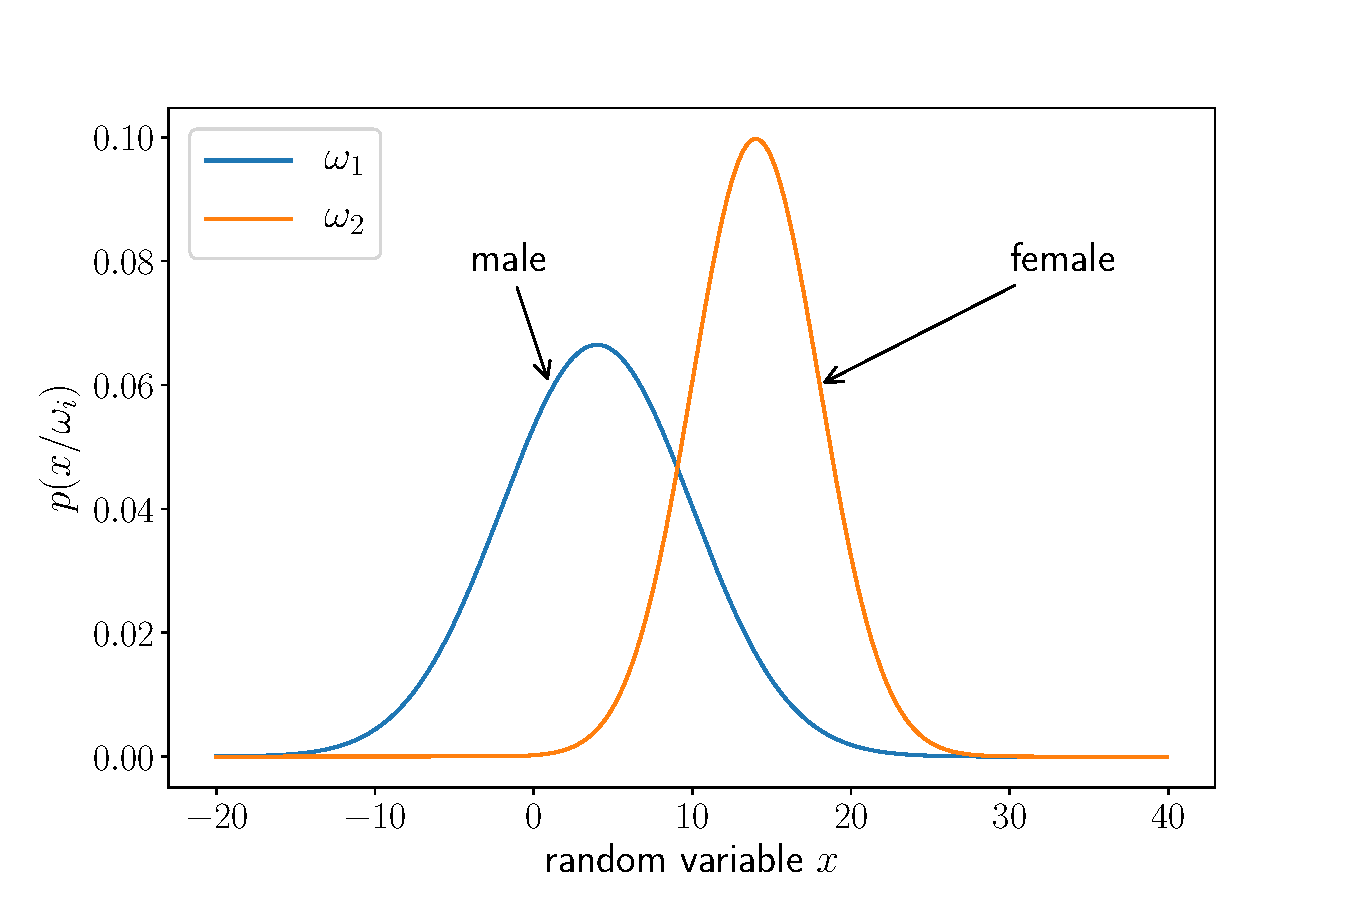
\includegraphics[width=6cm]{Figures/classProb}
\end{figure}
\end{frame}

\section{Applications}
\subsection{}

\begin{frame}{}
\begin{variableblock}{\centering \Large \textbf{\vspace{4pt}\newline Applications\vspace{4pt}}}{bg=slidecolor,fg=white}{bg=slidecolor,fg=white}
\end{variableblock}
\end{frame}

\begin{frame}{Machine Perception}
Build a machine that can recognize patterns:
\begin{itemize}
\item Speech recognition
\item Biometric recognition
\item Fingerprint identification
\item Face recognition
\item OCR (Optical Character Recognition)
\item DNA sequence identification
\item Autonomous navigation
\end{itemize}
\end{frame}

\begin{frame}{Applications: Speech Recognition}
\begin{figure}
\includegraphics[scale=0.8]{Figures/speechProc}
\end{figure}
\end{frame}

\begin{frame}{Applications: Biometric Recognition}
\vspace{-6pt}
\begin{multicols}{2}
\begin{itemize}
\item Fingerprint
\item Eyes - Iris recognition
\item Face recognition, identification/verification
\item Speech recognition
\item Finger geometry recognition
\item Hand geometry recognition
\item Signature recognition
\item Eyes - Retina recognition
\item Fingerprint recognition
\item Typing recognition
\item Gait recognition
\item DNA identification
\end{itemize}
\end{multicols}
\begin{figure}
\includegraphics[scale=0.8]{BiometricRecognition}
\end{figure}
\end{frame}

\begin{frame}{Applications: Fingerprint Identification}
\begin{columns}
\begin{column}{6cm}
\begin{itemize}
\item No two people have the same fingerprints
\item Fingerprints can solve crimes.
\item Fingerprints are impressions created by ridges on the skin.
\item Ridges form before a baby is born and maintain their pattern thoughout life.
\item As we grow, the pattern gets larger, but does not changes.
\end{itemize}
\end{column}
\begin{column}{5cm}
\begin{figure}
\includegraphics[scale=0.28]{Finger01.jpg}
\end{figure}
\end{column}
\end{columns}
\end{frame}

\begin{frame}{Applications: Fingerprint Identification}
How Fingerprint scanners record identifies:
\vspace{1.8cm}
\begin{figure}
\includegraphics[scale=0.3]{Figures/Finger02.png}
\end{figure}
\begin{tikzpicture}[remember picture,overlay]
  \node [text width=3cm,minimum height=1cm,minimum width=2cm,execute at begin node=\setlength{\baselineskip}{10pt}] at (2.6,6.4) {{\small \textbf{1.} Inidividuals index finger is pressed onto scanner}};
   \node [text width=4cm,minimum height=1cm,minimum width=2cm,execute at begin node=\setlength{\baselineskip}{10pt}] at (6.5,6.4) {{\small \textbf{2.} Scanner reads unique pattern plotting specific distinctions (minutiae)}};
    \node [text width=4cm,minimum height=1cm,minimum width=2cm,execute at begin node=\setlength{\baselineskip}{10pt}] at (10.6,6.15) {{\small \textbf{3.} Points are linked forming a pattern recorded as an algorithm used for comparison}};
\end{tikzpicture}
\end{frame}

\begin{frame}{Applications: Face Recognition}
\begin{figure}
\includegraphics[scale=0.75]{FaceRecog.jpg}
\end{figure}
\end{frame}

\begin{frame}{Applications: Face Recognition}
\begin{figure}
\includegraphics[scale=0.23]{FaceRecog01.png}
\end{figure}
\end{frame}

\begin{frame}{Applications: Optical Character Recognition (OCR)}
\begin{columns}
\begin{column}{5cm}
\begin{figure}
\includegraphics[height=5.5cm]{Figures/ocr.png}\\
\includegraphics[height=0.7cm]{Figures/ocr1.png}
\end{figure}
\end{column}
\begin{column}{8cm}
\begin{figure}
\includegraphics[height=1.5cm]{OCR02.jpg}
\end{figure}
\vspace{-0.5cm}
\begin{enumerate}
\item Differentiate word contours associated with Image.
\item Differentiate letter contours associated with word contours associated with word contour image.
\item Preprocess letter images according to trained OCR input
\item Consolidate predictions associated OCR model to text.
\end{enumerate}
\end{column}
\end{columns}
\end{frame}

\begin{frame}{Applications: DNA Identification}
\begin{figure}
\includegraphics[scale=0.4]{DNA01.jpg}
\end{figure}
\end{frame}

\begin{frame}{Applications: Autonomous Navigation}
\begin{figure}
\includegraphics[scale=0.9]{AutoCar}
\end{figure}
\end{frame}

\begin{frame}{Applications: Cancer Detection}
\begin{figure}
\includegraphics[scale=0.9]{CancerDetection}
\caption{Cancer detection and grading using microscopic tissue data}
\end{figure}
\end{frame}

\begin{frame}{Applications: Land Cover Detection}
\begin{figure}
\includegraphics[scale=0.9]{LandCover}
\caption{Land cover classification using satellite image}
\end{figure}
\end{frame}

\begin{frame}{Applications: License Plate Recognition}
\begin{figure}
\includegraphics[scale=0.9]{LPlates}
\caption{License plate recognition: US license plates}
\end{figure}
\end{frame}

\section{An Example}
\subsection{}

\begin{frame}{}
\begin{variableblock}{\centering \Large \textbf{\vspace{4pt}\newline A classic example to understand Pattern Classification\vspace{4pt}}}{bg=slidecolor,fg=white}{bg=slidecolor,fg=white}
\end{variableblock}
\end{frame}

\begin{frame}{An Example}
\vspace{-4pt}
\begin{itemize}
\item ``Sorting incoming Fish on a conveyor according to species using optical sensing\nocite{duda2012pattern,Omer2018}"
\item Species
\begin{itemize}
\item Sea bass
\item Salmon
\end{itemize}
\begin{figure}
\centering
\includegraphics[scale=0.4]{FishImg.jpg}
\end{figure}
\item Set up a camera and take some sample image to extract features
\begin{itemize}
\item Length
\item Lightness
\item Width
\item Number and shape of fins
\item Position of the mouth, etc.
\end{itemize}
\item This is the set of all suggested features to explore for use in our classifier.
\end{itemize}
\end{frame}

\begin{frame}{An Example}
\begin{columns}
\begin{column}{7cm}
\begin{itemize}
\item What can cause problems during sensing?
\begin{itemize}
\item {\color{mycolor2}lighting conditions}, 
\item position of fish on the conveyor belt, 
\item camera noise, etc.
\end{itemize}
\item Use a segmentation operation to {\color{mycolor2}isolate fishes} from one another and from the {\color{mycolor2}background}.
\item Information from a single fish is sent to a {\color{mycolor1}feature extractor} whose purpose is to reduce the data by measuring certain features.
\item The features are passed to a classifier.
\end{itemize}
\end{column}
\begin{column}{5cm}
\begin{figure}
\includegraphics[scale=0.5]{Ch0214}
\end{figure}
\end{column}
\end{columns}
\end{frame}

%\begin{frame}{An Example}
%\begin{figure}
%\includegraphics[scale=0.55]{Ch0214}
%\end{figure}
%\end{frame}

\begin{frame}{An Example: Classification}
\begin{itemize}
\item Select the length of the fish as a possible feature for discrimination
\end{itemize}
\begin{figure}
\includegraphics[scale=0.75]{Figures/Ch0101}
\caption{Histograms for the length feature for the two categories. No single threshold value $l^*$ (decision boundary) will serve to unambiguously discriminate between the two categories; using length alone, we will have some errors. The value $l*$ marked will lead to the smallest number of errors, on average.}
\end{figure}
\end{frame}

\begin{frame}{An Example: Classification}
\begin{itemize}
\item The length is a poor feature alone
\item Select the lightness as a possible feature
\end{itemize}
\begin{figure}
\includegraphics[scale=0.8]{Figures/Ch0102}
\caption{Histograms for the lightness feature for the two categories. No single threshold value $x^*$ (decision boundary) will serve to unambiguously discriminate between the two categories; using lightness alone, we will have some errors. The value $x^*$  marked will lead to the smallest number of errors, on average.}
\end{figure}
\end{frame}

\begin{frame}{Threshold decision boundary and cost relationship}
\begin{itemize}
\item Move our decision boundary toward smaller values of lightness in order to \textit{\color{mycolor2}minimize the cost} (reduce the number of sea bass that are classified salmon)\\
\vspace{14pt}
\begin{center}
{\Huge $\Downarrow$}\\
\vspace{14pt}
Task of decision theory
\end{center}
\end{itemize}
\end{frame}

\begin{frame}{An Example: Feature vector}
\begin{itemize}
\item Adopt the lightness and add the width of the fish
\item We can use two features in our decision:
\begin{itemize}
\item lightness: $x_1$
\item width: $x_2$
\end{itemize}
\item Each fish image is now represented as a point ({\color{mycolor2}feature vector}) ${\rm x}$ in two-dimensional  {\color{mycolor2}feature space}.
\end{itemize}
\vspace{-0.5cm}
\begin{columns}
\begin{column}{6cm}
\begin{figure}
\includegraphics[scale=0.75]{Ch0103}
\end{figure}
\end{column}
\begin{column}{4cm}
$~~~{\rm x}=[x_1~~~~x_2]^T$\\
~~~~~~~~~$\downarrow$~~~~~$\downarrow$\\
Lightness~~ Width
\end{column}
\end{columns}
\end{frame}

\begin{frame}{An Example: Feature vector}
\begin{itemize}
\setlength{\itemsep}{12pt}
\item We might add other features that are not correlated with the ones we already have. A precaution should be taken not to reduce the performance by adding such ``noisy features''.
\item Does adding more features always improve the results?
\begin{itemize}
\item unreliable features.
\item Be careful about correlations with existing features.
\item Be careful about measurement costs.
\item Be careful about noise in the measurements.
\end{itemize} 
\item Is there some \textit{\color{mycolor2}curse} for working in very high dimensions?
\end{itemize}
\end{frame}

\begin{frame}{An Example: Feature vector}
\begin{itemize}
\item Ideally, the best decision boundary should be the one which provides an optimal performance.
\begin{figure}
\includegraphics[scale=1.1]{Ch0104}
\end{figure}
\end{itemize}
\end{frame}

\begin{frame}{An Example: Issue of generalization}
\begin{itemize}
\item How can we mange the \textit{\color{mycolor2}tradeoff} between complexity of decision rules and their performance to unknown samples?
\item Our satisfaction is premature because the central aim of designing a classifier is to correctly classify novel input\\
\vspace{14pt}
\begin{center}
{\Huge $\Downarrow$}\\
\vspace{14pt}
Issue of generalization
\end{center}
\end{itemize}
\end{frame}

\begin{frame}{An Example: Decision Boundary}
\begin{figure}
\includegraphics[scale=1.1]{Figures/Ch0105}
\caption{The decision boundary shown might represent the optimal trade of between performance on the training set and simplicity of classifier.}
\end{figure}
\end{frame}

\begin{frame}{More on Complexity}
\begin{figure}
\includegraphics[scale=1]{Reg01}
\caption{Regression example: plot of 10 sample points for the input variable $x$ along with the corresponding target variable $t$. Green curve is the true function that generated the data.}
\end{figure}
\end{frame}

\begin{frame}{More on Complexity}
\begin{figure}
\includegraphics[scale=0.9]{Reg02}
\caption{Polynomial curve fitting: plots of polynomials having various orders, shown as red curves, fitted to the set of 10 sample points}
\end{figure}
\end{frame}

\begin{frame}{More on Complexity}
\begin{figure}
\includegraphics[scale=1]{Reg03}
\caption{Polynomial curve fitting: plots of 9'th order polynomials fitted to 15 and 100 sample points.}
\end{figure}
\end{frame}

\section{PR Systems}
\subsection{}

\begin{frame}{}
\begin{variableblock}{\centering \Large \textbf{\vspace{4pt}\newline Pattern Recognition System and Design Cycle\vspace{4pt}}}{bg=slidecolor,fg=white}{bg=slidecolor,fg=white}
\end{variableblock}
\end{frame}


\begin{frame}{Pattern Recognition Models}
There are three main models of pattern recognition:
\setlength{\itemsep}{12pt}
\begin{itemize}
\item {\color{mycolor1}Statistical:} 
\begin{itemize}
\item To identify where specific piece belongs (for example, whether it is a cake or not).
\item Use of statistics to learn from examples.
\end{itemize}
\item {\color{mycolor1}Syntactic/Structural:} 
\begin{itemize}
\item To define a more complex relationship between elements taking into account more complex interrelationships between attributes.
\item Looks at clear structure in the patterns.
\item An example of this would be diagnosis of the heart with ECG measurements.
\end{itemize}
\item {\color{mycolor1}Template Matching:}
\begin{itemize}
\item To match the object's features with the predefined template and identify the object by proxy. 
\item One of the uses of such model is plagiarism checking.
\end{itemize} 
\end{itemize}
\end{frame}

\begin{frame}{Pattern Recognition Systems}
\begin{figure}
\includegraphics[width=6.7cm]{Figures/PRsystem2}
\caption{Object/Process diagram of a pattern recognition system}
\end{figure}
\end{frame}

\begin{frame}{Pattern Recognition Systems}
\begin{itemize}
\setlength{\itemsep}{6pt}
\item {\color{mycolor2}Data acquisition and sensing:}
\begin{itemize}
\item Use of transducer (camera or microphone)
\item Measurements of physical variables.
\item Important issues: bandwidth, resolution, sensitivity,
distortion, SNR, latency, etc.
\end{itemize}
\item {\color{mycolor2}Pre-processing:}
\begin{itemize}
\item  Removal of noise in data.
\item Isolation of patterns of interest from the background.
\item Segmentation and grouping
\end{itemize}
\item {\color{mycolor2}Feature extraction:}
\begin{itemize}
\item Finding a new representation in terms of features.
\item Features should be well separated and should not overlap (Discriminative features )
\item Invariant features with respect to translation, rotation and scale.
\item Depends on the characteristics of the problem domain. Simple to extract, invariant to irrelevant transformation insensitive to noise.
\end{itemize} 
\end{itemize}
\end{frame}

\begin{frame}{Pattern Recognition Systems}
\begin{itemize}
\setlength{\itemsep}{6pt}
\item {\color{mycolor2} Model learning and estimation:}
\begin{itemize}
\item Learning a mapping between features and pattern groups and categories.
\item Unsatisfied with the performance of classifier and want to jump to another class of model
\end{itemize}
\item {\color{mycolor2}Classification:}
\begin{itemize}
\item  Using features and learned models to assign a pattern to a category.
\end{itemize}
\item {\color{mycolor2}Post-processing:}
\begin{itemize}
\item Evaluation of confidence in decisions.
\item Exploitation of context to improve performance.
\item Combination of experts.
\end{itemize} 
\end{itemize}
\end{frame}

\section{Design Cycle}
\subsection{}

\begin{frame}{The Design Cycle}
\begin{figure}
\includegraphics[width=\textwidth]{Figures/DesignCycle}
\caption{Design cycle}
\end{figure}
\begin{itemize}
\item {\color{mycolor2}Data Collection}
\begin{itemize}
\item Collecting training and testing data.
\item How do we know when we have collected an adequately large and representative set of examples for training and testing the system?
\end{itemize}
\end{itemize}
\vspace{2cm}
\end{frame}

\begin{frame}{The Design Cycle}
\begin{figure}
\includegraphics[width=\textwidth]{Figures/DesignCycle}
\caption{Design cycle}
\end{figure}
\vspace{-20pt}
\begin{itemize}
\setlength{\itemsep}{12pt}
\item {\color{mycolor2}Feature Selection}
\begin{itemize}
\item Domain dependence and prior information.
\item Computational cost and feasibility.
\item Discriminative features.
\begin{itemize}
\item Similar values for similar patterns.
\item Different values for different patterns.
\end{itemize}
\item Invariant features with respect to translation, rotation and
scale.
\item Robust features with respect to occlusion, distortion,
deformation, and variations in environment.
\end{itemize}
\end{itemize}
\end{frame}

\begin{frame}{The Design Cycle}
\begin{figure}
\includegraphics[width=\textwidth]{Figures/DesignCycle}
\caption{Design cycle}
\end{figure}
\vspace{-20pt}
\begin{itemize}
\item {\color{mycolor2}Model selection}
\begin{itemize}
\item Domain dependence and prior information.
\item Definition of design criteria.
\item Parametric vs. non-parametric models.
\item Handling of missing features.
\item Computational complexity.
\item Types of models: templates, decision-theoretic or statistical, syntactic or structural, neural, and hybrid.
\item How can we know how close we are to the true model underlying the patterns?
\end{itemize}
\end{itemize}
\end{frame}

\begin{frame}{The Design Cycle}
\begin{figure}
\includegraphics[width=\textwidth]{Figures/DesignCycle}
\caption{Design cycle}
\end{figure}
\vspace{-12pt}
\begin{itemize}
\item {\color{mycolor2}Training}
\begin{itemize}
%\setlength{\itemsep}{3pt}
\item How can we learn the rule from data?
\item Supervised learning: a teacher provides a category label or
cost for each pattern in the training set.
\item Unsupervised learning: the system forms clusters or natural groupings of the input patterns.
\item Reinforcement learning: no desired category is given but the teacher provides feedback to the system such as the decision is right or wrong.
\end{itemize}
\end{itemize}
\end{frame}

\begin{frame}{The Design Cycle}
\begin{figure}
\includegraphics[width=\textwidth]{Figures/DesignCycle}
\caption{Design cycle}
\end{figure}
\vspace{-12pt}
\begin{itemize}
\setlength{\itemsep}{12pt}
\item {\color{mycolor2}Evaluation}
\begin{itemize}
\setlength{\itemsep}{2pt}
\item How can we estimate the performance with training
samples?
\item How can we predict the performance with future data?
\item Problems of overfitting and generalization.
\end{itemize}
\item {\color{mycolor2}Computational Complexity}
\begin{itemize}
\setlength{\itemsep}{2pt}
\item What is the trade-off between computational ease and performance?
\item How an algorithm scales as a function of the number of features, patterns or categories?
\end{itemize}
\end{itemize}
\end{frame}

\begin{frame}{Different Learning Approaches}
\begin{itemize}
\setlength{\itemsep}{8pt}
\item {\color{mycolor2}Supervised learning/Classification}
\begin{itemize}
\item A teacher provides a category label or cost for each pattern in the training set
\end{itemize}
\item {\color{mycolor2}Unsupervised learning/Clustering}
\begin{itemize}
\item The system forms clusters or "natural groupings" of the input pattern (no explicit teacher)
\end{itemize}
\item {\color{mycolor2}Semi-supervised learning}
\begin{itemize}
\item Semi-supervised learning is the problem of learning from examples for which you have labels for only a (small) subset.
\end{itemize}
\item {\color{mycolor2}Reinforcement learning}
\begin{itemize}
\item Learning with critic, no desired category is known; instead, the only teaching feedback is that the tentative category is right or wrong. It utilizes reward function to learn. Ex: Autonomous driving
\end{itemize}
\end{itemize}
\end{frame}

\section{References}
\subsection{}
\begin{frame}[allowframebreaks]{References}
\linespread{1}
\footnotesize
\printbibliography[heading=none]
\end{frame}
{
\setbeamertemplate{logo}{}
\makeatletter
\setbeamertemplate{footline}{
        \leavevmode%
  
  % First line.
  \hbox{%
  \begin{beamercolorbox}[wd=.2\paperwidth,ht=\beamer@decolines@lineup,dp=0pt]{}%
  \end{beamercolorbox}%
  \begin{beamercolorbox}[wd=.8\paperwidth,ht=\beamer@decolines@lineup,dp=0pt]{lineup}%
  \end{beamercolorbox}%
  } %
  % Second line.
  \hbox{%
  \begin{beamercolorbox}[wd=\paperwidth,ht=\beamer@decolines@linemid,dp=0pt]{linemid}%
  \end{beamercolorbox}%
  } %
  % Third line.
  \hbox{%
  \begin{beamercolorbox}[wd=.1\paperwidth,ht=\beamer@decolines@linebottom,dp=0pt]{}%
  \end{beamercolorbox}%
  \begin{beamercolorbox}[wd=.9\paperwidth,ht=\beamer@decolines@linebottom,dp=0pt]{linebottom}%
  \end{beamercolorbox}%
  }%
        }
\makeatother

\begin{frame}
\centering
\includegraphics[width=0.4\paperwidth]{queries.jpg}\\
\includegraphics[width=0.45\paperwidth]{thank_you.png}
\end{frame}
}


%\graphicspath{{Figures/}}

\title{\fontsize{33}{45}{\huge Pattern Classification\newline{\large Lecture 02: Feature Extraction}\newline \vspace{8pt} \Large \vspace{-1.1cm}}}

\vspace{0.5cm}
\author{\vspace{0.4cm}\\\large{\bf Kundan Kumar\\\url{https://github.com/erkundanec/PatternClassification}}
%Associate Professor\\Department of ECE}
}
% - Give the names in the same order as the appear in the paper.
% - Use the \inst{?} command only if the authors have different
%   affiliation.
%\vspace{1cm}
\institute[Indian Institute of Technology Kharagpur] % (optional, but mostly needed)
{
\vspace{1.8cm}
%\includegraphics[height=.17\textheight]{SOAlogo.png}\\
% Faculty of Engineering (ITER)\\ S`O'A Deemed to be University, Bhubaneswar, India-751030\\


 \copyright\  2020 Kundan Kumar, All Rights Reserved\\
  \vspace{-1.1cm}}
% - Use the \inst command only if there are several affiliations.
% - Keep it simple, no one is interested in your street address.
\date{}
% To remove page number from a perticular slide
{
\setbeamertemplate{logo}{}
\makeatletter
\setbeamertemplate{footline}{
        \leavevmode%
  
  % First line.
  \hbox{%
  \begin{beamercolorbox}[wd=.2\paperwidth,ht=\beamer@decolines@lineup,dp=0pt]{}%
  \end{beamercolorbox}%
  \begin{beamercolorbox}[wd=.8\paperwidth,ht=\beamer@decolines@lineup,dp=0pt]{lineup}%
  \end{beamercolorbox}%
  } %
  % Second line.
  \hbox{%
  \begin{beamercolorbox}[wd=\paperwidth,ht=\beamer@decolines@linemid,dp=0pt]{linemid}%
  \end{beamercolorbox}%
  } %
  % Third line.
  \hbox{%
  \begin{beamercolorbox}[wd=.1\paperwidth,ht=\beamer@decolines@linebottom,dp=0pt]{}%
  \end{beamercolorbox}%
  \begin{beamercolorbox}[wd=.9\paperwidth,ht=\beamer@decolines@linebottom,dp=0pt]{linebottom}%
  \end{beamercolorbox}%
  }%
        }
\makeatother
\begin{frame}
\titlepage
\end{frame}
}

\section{Feature Extraction}
\subsection{}
%\begin{frame}{}
%\begin{variableblock}{\centering \Large \textbf{\vspace{4pt}\newline Feature Extraction\vspace{4pt}}}{bg=slidecolor,fg=white}{bg=slidecolor,fg=white}
%\end{variableblock}
%\end{frame}

\begin{frame}{Topics to be covered}
\begin{itemize}
%\setlength{\itemsep}{-2pt}
\item Boundary Representation\nocite{gonzalez2002digital}
\begin{itemize}
\setlength{\itemsep}{-2pt}
\item Boundary (Border) following
\item Chain codes
\item Polynomial Approximation
\item Signatures
\item Boundary Segments
\item Skeletons
\end{itemize}
\item Boundary Descriptors
\begin{itemize}
\setlength{\itemsep}{-2pt}
\item Some Simple Descriptors
\item Shape Numbers
\item Fourier Descriptors
\item Statistical Moments
\end{itemize}
\item Regional Descriptors
\begin{itemize}
\setlength{\itemsep}{-2pt}
\item Texture: Moment Invariants
\item Texture: GLCM, LBP
\end{itemize}
\item Transformed domain features
\begin{itemize}
\item 2D-Gabor filter features
\end{itemize}
\end{itemize}
\end{frame}

\begin{frame}{Introduction to feature extraction}
\begin{itemize}
\item Scale invariant
\item Translation invariant
\item Rotation invariant
\item Luminance invariant
\end{itemize}
\vspace{-12pt}
\begin{figure}
\includegraphics[height=4cm]{ArcCircle.png}~~~~
\includegraphics[height=4cm]{ArcCircle01.jpg}
\end{figure}
\end{frame}

\begin{frame}{Feature extraction from an ECG signal}
\begin{figure}
\includegraphics[height = 5cm]{ECG02.png}\\
\includegraphics[width = 0.5\textwidth]{Figures/ECG01a.png}~~~
\includegraphics[width = 0.5\textwidth]{Figures/ECG01b.png}
\end{figure}
\end{frame}

\begin{frame}{Good features and Bad features}
\begin{itemize}
\item Extract features which are good for {\color{maroon}classification}.
\item {\color{maroon}Good features}:
\begin{itemize}
\item Objects from the same class have similar feature values
\item Objects from different classes have different values.
\end{itemize}
\item {\color{maroon}Bad Features:} features simply do not contain the information needed to separate the classes, doesn't matter how much effort you put into designing the classifier.
\end{itemize}
\begin{figure}
\includegraphics[scale=0.7]{Figures/goodbadFeatures}
\end{figure}
\end{frame}

\begin{frame}{Feature separability}
\begin{figure}
\includegraphics[scale=0.63]{Figures/FeatureSep}
\end{figure}
\end{frame}

\begin{frame}{Nature of separating plane?}
\begin{itemize}
\item For 2 dimensional feature space -- {\color{maroon}line}
\item For 3 dimensional feature space -- {\color{maroon}plane}
\item For more than 3 dimensional feature space -- {\color{maroon}hyperplane}
\end{itemize}
\begin{figure}
\includegraphics[scale=0.36]{Figures/Plane.png}
\end{figure}
\end{frame}

\begin{frame}{Labeled features}
\begin{columns}
\begin{column}{5cm}
\begin{figure}
\includegraphics[scale=0.65]{Figures/label.png}
\end{figure}
\end{column}
\begin{column}{5cm}
\[\begin{array}{*{20}{c}}
{\left. {\begin{array}{*{20}{c}}
{{f_1}}\\
{{f_2}}\\
{{f_3}}
\end{array}} \right\} \in {C_1}}\\
{\left. {\begin{array}{*{20}{c}}
{{f_4}}\\
{{f_5}}\\
{{f_6}}\\
{{f_7}}
\end{array}} \right\} \in {C_2}}
\end{array}\]
\end{column}
\end{columns}
\begin{itemize}
\item In general, we use labeled features for supervised learning.
\end{itemize}
\end{frame}

\begin{frame}{Some property of features}
\begin{itemize}
\item The mapping from pattern to features that is unique whereas mapping from feature vector to pattern is not immediate.
\item So many patterns may be matched to the same feature of vector.
\item In pattern recognition, we never talk about a single pattern. We always talk about {\color{maroon}feature vector}.
\end{itemize}
\vspace{12pt}
\textbf{Types of Boundary Features:}
\begin{enumerate}
\item Boundary features/Descriptors
\item Region features/Descriptors
\end{enumerate}
\end{frame}

\section{Boundary Representation}
\subsection{}
\begin{frame}{}
\begin{variableblock}{\centering \Large \textbf{\vspace{4pt}\newline Boundary Representation\vspace{4pt}}}{bg=slidecolor,fg=white}{bg=slidecolor,fg=white}
\end{variableblock}
\begin{figure}
\centering
\includegraphics[width=4cm]{Figures/Paper0.png}\\\vspace{4pt}
\includegraphics[width=2.5cm]{Figures/Paper1.jpg}~~~~~~
\includegraphics[width=2.5cm]{Figures/Paper2.jpg}~~~~~~
\includegraphics[width=2.5cm]{Figures/Paper3}
\end{figure}
\end{frame}

\begin{frame}{Binary Images}
\begin{figure}
\includegraphics[scale=0.35]{Binary01.png}\\
\includegraphics[scale=0.35]{Binary02.png}
\caption{Binary Images}
\end{figure}
\end{frame}

\begin{frame}{Boundary (Border) algorithm}
\begin{itemize}
\item Assume a binary image in which object and background points are labeled 1 and 0, respectively.
\item Assume images are padded with the border of 0s to avoid object merging with the image border
\end{itemize}
\begin{figure}
\includegraphics[scale=0.9]{Feature06}\\
\includegraphics[scale=0.9]{Feature07}
\caption{Illustration of the first few steps in the {\color{maroon}boundary-following algorithm}}
\end{figure}
\end{frame}

\begin{frame}{Boundary algorithm (Moore boundary tracking algorithm)}
\begin{footnotesize}
\begin{itemize}
\item[1.] Let the starting point, $b_0$ be the \textit{uppermost, leftmost} point in the image that is labeled 1. Denote by $c_0$ the \textit{west} neighbor of $b_0$.
Clearly, $c_0$ always is a background point. Examine the 8-neighbors of $b_0$, starting at $c_0$ and proceeding in a clockwise direction. Let $b_1$ denote
the \textit{first} neighbor encountered whose value is 1, and let $c_1$ be the (back-ground) point immediately preceding $b_1$ in the sequence. Store the locations of $b_0$ and $b_1$ for use in Step 5.
\item[2.] Let $b=b_1$ and $c=c_1$.
\item[3.] Let the 8-neighbors of $b$, starting at $c$ and proceeding in a clockwise direction, be denoted by $n_1,n_2,\ldots,n_8$. Find the first $n_k$ labeled 1.
\item[4.] Let $b=n_k$ and $c=n_{k-1}$
\item[5.] Repeat Step 3 and 4 until $b=b_0$ and the next boundary point found in $b_1$. The sequence of $b$ points found when the algorithm stops constitutes the set of ordered boundary points.
\end{itemize}
\end{footnotesize}
\end{frame}

\begin{frame}{Boundary algorithm - stopping criterion}
\begin{figure}
\includegraphics[scale=1.1]{Feature08}
\caption{Illustration of an erroneous result when the stopping rule is such that boundary-following stops when the starting point, $b_0$, is encountered again}
\end{figure}
\end{frame}

\begin{frame}{Boundary representation: Chain Codes}
\begin{itemize}
\item In order to represent a boundary, it is useful to compact the raw data ({\color{mycolor2}list of boundary pixels})
\item {\color{mycolor1}Chain codes:} list of segments with defined length and direction
\begin{itemize}
\item 4-directional chain codes
\item 8-directional chain codes
\end{itemize}
\begin{figure}
\includegraphics[scale=1]{Feature01}
\caption{Direction numbers for (a) 4-directional chain code, and (b) 8-directional chain code}
\end{figure}
\end{itemize}
\end{frame}

\begin{frame}{Boundary representation: Chain Codes}
\begin{itemize}
\item It may be useful to downsample the data before computing the chain code
\begin{itemize}
\item to reduce the code dimension
\item to remove small detail along the boundary
\end{itemize}
\begin{figure}
\includegraphics[scale=0.75]{Feature02}
\caption{(a) Digital boundary with resampling grid superimposed, (b) Result of resampling, (c) 8-directional chain-coded boundary.}
\end{figure}
\item Can you draw 4-directional chain-coded boundary?
\end{itemize}
\begin{tikzpicture}[remember picture,overlay]
    \node (img1) at (10.5,5.5) {\includegraphics[scale=0.7]{Figures/Feature01a}};
\end{tikzpicture}
\end{frame}

\begin{frame}{Boundary representation: Chain Codes}
\vspace{2.3cm}
\begin{figure}
\includegraphics[scale=0.7]{Feature09}~~~
\onslide<2->{\includegraphics[scale=0.235]{Feature10_1.png}~~~}
\onslide<3->{\includegraphics[scale=0.65]{Feature10}}
\end{figure}
\begin{tikzpicture}[remember picture,overlay]
\node (img1) at (2,6.5) {\includegraphics[scale=0.75]{Figures/Feature01b}};
\onslide<4->{\node (img1) at (7,6.5) {{\color{mycolor1}Chain code:} 0033333323221211101101};}
\end{tikzpicture}
\end{frame}

%\begin{frame}{Boundary representation: Chain Codes}
%\begin{itemize}
%\item Chain codes are used to represent a boundary by a connected sequence of straight-line segments of specified length and direction.
%\item The direction of each segment is coded by using a numbering scheme that we discussed.
%\end{itemize}
%\end{frame}

\begin{frame}{Boundary representation: Differential Chain Code}
\begin{itemize}
\item The chain code of a boundary depends on the starting point.
\begin{itemize}
\item normalize with respect to the starting point (circular sequence)
\item the new starting point is the one who gives a sequence of numbers giving the \textit{\color{mycolor1}smallest/largest integer}.
\end{itemize}
\item Normalize with respect to rotation:
\begin{itemize}
\item First difference can be used
\item E.g., $10103322\Rightarrow 3133030$ (counting CCW) and adding the last transition (circular sequence: $2\Rightarrow 1$)\\ $\Rightarrow$ 31330303 (\textit{\color{mycolor2}Differential Chain Code})\\ $\Rightarrow$ 03033133 (\textit{\color{mycolor2}Independent of starting point}, \textit{\color{mycolor1} i.e., rotation invariant})
\end{itemize}
\begin{figure}
\includegraphics[scale=0.8]{Feature01}
\end{figure}
\end{itemize}
\end{frame}

\begin{frame}{Differential Chain Code}
\begin{figure}
\includegraphics[scale=1]{Feature02}
\end{figure}
\onslide<1>{Can you write the Differential Chain Code?
\begin{itemize}}
\onslide<2->{\item Chain code: 0766666453321212}
\onslide<3->{\item Differential chain code: 7700006160771716}
\onslide<4->{\item Differential chain code (rotation invariant): 0000616077171677}
\end{itemize}
\end{frame}


\begin{frame}{Differential Chain Code: Validation}
\begin{figure}
\includegraphics[scale=0.9]{Figures/Feature02a}~~~
\includegraphics[scale=0.9]{Figures/Feature02b}~~~
\includegraphics[scale=0.9]{Figures/Feature02c1}
\end{figure}
\onslide<1>{Can you write the Differential Chain Code?
\begin{itemize}}
\onslide<2->{\item Chain code: 0707065444442311}
\onslide<3->{\item Differential chain code: 7171677000061607}
\onslide<4->{\item Differential chain code: 0000616077171677 (validated)}
\onslide<5->{\item Is the differential chain code is invariant to rotation at any angle? ({\color{mycolor2}HW})}
\end{itemize}
\end{frame}

%\begin{frame}{Polygonal Approximation: Minimum-Perimeter polygon}
%\begin{figure}
%\includegraphics[scale=0.7]{Feature03}
%\end{figure}
%\end{frame}

\begin{frame}{Polygonal Approximation}
\begin{itemize}
\begin{small}
\item A digital boundary can be approximated with arbitrary accuracy by a polygon.
\item In practice, the goal of polygonal approximation is to capture the ``essence'' of the {\color{mycolor1}boundary shape} with the {\color{mycolor3}fewest possible polygonal segments}.
\begin{itemize}
\item Minimum-perimeter polygon
\item Splitting technique
\end{itemize}
\end{small}
\end{itemize}
\begin{figure}
\includegraphics[scale=0.43]{Feature03}
\caption{(a) An object boundary (black curve). (b) Boundary enclosed by cells (in gray). (c) Minimum-perimeter polygon obtained by allowing the boundary to shrink. The vertices of the polygon are created by the corners of the inner and outer walls of the gray region.}
\end{figure}
\end{frame}

\begin{frame}{Polygonal Approximation: Minimum-Perimeter Polygon}
\begin{figure}
\includegraphics[scale=0.75]{Feature11}
\caption{(a) Region (dark gray) resulting from enclosing the original boundary by cells.
(b) Convex (white dots) and concave (black dots) vertices obtained by following the boundary of the dark
gray region in the counterclockwise direction. (c) Concave vertices (black dots) displaced to their diagonal
mirror locations in the outer wall of the bounding region; the convex vertices are not changed. The MPP
(black boundary) is superimposed for reference.}
\end{figure}
\end{frame}

\begin{frame}{Polygonal Approximation: Splitting Technique}
\begin{itemize}
\item One approach to boundary segment splitting is 
to subdivide a segment successively into two 
part until a \textit{\color{mycolor1}specified criterion} is satisfied.
\begin{figure}
\includegraphics[scale=0.7]{Ch0001}
\caption{(a) Original boundary, (b) Boundary divided into segments based on extreme points, (c) Joining of vertices, (d) Resulting polygon}
\end{figure}
\end{itemize}
\end{frame}

\begin{frame}{Polygonal Approximation: Splitting Technique}
\begin{itemize}
\item For a closed boundary, the best starting points 
usually are two farthest points in the boundary.
\item Farthest point can be obtained by \textit{\color{mycolor1}Karhunen-Loeve transform (KLT)}.
\item The maximum perpendicular distance from a boundary segment to the line joining its two end points not exceed a preset threshold.
\item Splitting procedure with a threshold equal to 
0.25 times the length of line $ab$.
\end{itemize}
\end{frame}

\begin{frame}{Signatures}
\begin{itemize}
\item A signature is a 1-D representation of a boundary (which is a 2-D thing): it should be easier to describe.\\ e.g., distance form the centroid vs angle.
\begin{figure}
\includegraphics[scale=0.6]{Ch0002}
\caption{Distance-versus-angle signatures. (a) $r(\theta)$, is constant, (b) the signature consists of repetitions of the pattern $r(\theta)=Asec(\theta)$ for $0\leq \theta \leq \pi/4$ and $r(\theta)=Acsc(\theta)$ for $\pi/4<\theta\leq \pi/2$}
\end{figure}
\end{itemize}
\end{frame}

\begin{frame}{Signatures}
\begin{itemize}
\setlength{\itemsep}{12pt}
\item Signatures are invariant to translation, but variant to rotation.
\item Invariant to rotation: depends on the starting point
\begin{itemize}
\item the starting point could be the farthest point from the \textit{\color{mycolor1}centroid}. 
\end{itemize}
\item Scaling varies the amplitude of the signature
\begin{itemize}
\item invariance can be obtained by normalizing between 0 and 1, or
\item by dividing by the variance of the signature (does not work on circle)
\end{itemize}
\end{itemize}
\end{frame}

\begin{frame}{Boundary Segments}
\begin{itemize}
\item Decomposing a boundary into segments often 
is useful.
\item Decomposition reduces the boundary's 
complexity and thus simplifies the description 
process.
\item In this case use of the \textit{\color{mycolor1}convex hull} of the region 
enclosed by the boundary is a powerful tool for 
robust decomposition of the boundary.
\end{itemize}
\end{frame}

\begin{frame}{Boundary Segments}
\begin{itemize}
\item \textit{\color{mycolor1} Convex hull} $H$ of an arbitrary set $S$ is the 
smallest convex set containing $S$.
\item The set difference $H-S$ is called the \textit{\color{mycolor1} convex 
deficiency} $D$ of the set $S$.
\item Note that in principle, this scheme is 
independent of region size and orientation.
\end{itemize}
\begin{figure}
\includegraphics[scale=0.7]{Feature12}
\caption{(a) A region, $S$, and its convex deficiency (shaded). (b) Partitioned boundary.}
\end{figure}
\end{frame}

\begin{frame}{Skeletonization}
\begin{itemize}
\item One way to represent a shape is to reduce it to a graph, by obtaining its \textit{\color{mycolor1}skeleton} via thinning (\textit{\color{mycolor1}skeletonization})
\item \textit{\color{mycolor2}MAT (Medial axis transformation)} is composed by all the points which have more than one 
closest boundary points (``\textit{\color{mycolor2}prairie fire concept}'')
\end{itemize}
\begin{figure}
\subfigure[]{\includegraphics[scale=0.6]{Feature13}}~~~
\subfigure[]{\includegraphics[scale=0.4]{Feature14}}
\caption{(a) Medial axes (dashed) of three simple regions,(b) Human leg bone and skeleton of the region}
\end{figure}
\end{frame}

\section{Boundary Descriptors}
\subsection{}

\begin{frame}{}
\begin{variableblock}{\centering \Large \textbf{\vspace{4pt}\newline Boundary Features/Descriptors\vspace{4pt}}}{bg=slidecolor,fg=white}{bg=slidecolor,fg=white}
\end{variableblock}
\end{frame}

\begin{frame}{Simple descriptors}
\vspace{-4pt}
\begin{itemize}
\item \textit{\color{mycolor1}length} of a boundary is one of its simplest descriptors.
\begin{itemize}
\item The number of pixels along a boundary gives a rough approximation of its length.
\item For a chain coded curve with unit spacing:
\[\boxed{\textit{\color{mycolor1}length} ={\rm Horizontal}+{\rm Vertical}+\sqrt{2}\times {\rm Diagonal}}\]
\end{itemize}
%where, Horizontal is the no. horizontal components, Vertical is the no. of vertical components, and Diagonal is the no. of diagonal components.
\item \textit{\color{mycolor1}diameter} (length of the major axis)
\[\boxed{{\rm Diam}(B)=\max_{i,j}{[D(p_i,p_j)]}}\]
\item The \textit{\color{mycolor1}minor axis} of a boundary is defined as the 
line perpendicular to the \textit{\color{mycolor1}major axis}.
\item \textit{\color{mycolor1}Basic rectangle} (formed by the major and the minor axis; 
encloses the boundary) and its
\[\boxed{{\sf \color{mycolor2} eccentricity}=\frac{\it \sf major~axis}{\it \sf minor~axis}}\]
\end{itemize}
\end{frame}

\begin{frame}{Shape Number}
\begin{itemize}
\item {\color{mycolor1}Shape number:} the first difference as {\color{mycolor2}smallest magnitude} (treating the chain code as a circular sequence)
\item {\color{mycolor1}Order of a shape:} the number of digits in Shape number.
\end{itemize}
\vspace{-0.5cm}
\begin{figure}
\includegraphics[scale=0.64]{Feature04}~~~
\includegraphics[scale=0.64]{Feature01}
\end{figure}
\end{frame}

\begin{frame}{Shape Number}
\begin{itemize}
\item It is advisable to normalize the grid orientation by {\color{mycolor4}aligning} the chain code grid {\color{mycolor4}to the basic rectangle}.
\end{itemize}
\begin{figure}
\includegraphics[scale=0.7]{Figures/Feature05}~~
\includegraphics[scale=1]{Figures/Feature05e}~~
\includegraphics[scale=1]{Figures/Feature05f}
\end{figure}
\begin{figure}
\includegraphics[scale=1]{Feature05a}
\end{figure}
\end{frame}

\begin{frame}{Fourier Descriptors}
\begin{figure}
\includegraphics[scale=1]{Feature30}
\caption{A digital boundary and its representation as a complex sequence. The point $(x_0,y_0)$ and $(x_1,y_1)$ shown are (arbitrarily) the first two points in the sequence.}
\end{figure}
\end{frame}

\begin{frame}{Fourier Descriptors}
\begin{itemize}
\item Each coordinate pair treat as a complex number
\[\boxed{s(k)=x(k)+jy(k)}\]
for $k=0,1,2,\ldots, N-1$.
\item The discrete Fourier transform (DFT) of $s(k)$ is
\[\boxed{a(u) = \sum\limits_{k = 0}^{N - 1} {s(k){e^{ - j2\pi uk/N}}} }\]
for $u=0,1,2,\ldots,N-1$
\item $a(u)$ are Fourier Descriptors.
\end{itemize}
\end{frame}

\begin{frame}{Statistical moments}
\vspace{-4pt}
\begin{figure}
\includegraphics[scale=0.7]{Feature27}
\end{figure}
\begin{itemize}
\item Once a boundary is described as a 1-D function, {\color{mycolor2}statistical moments} (mean, variance, and a few higher-order central moments) can be used to describe it.
\[\boxed{{\mu _n}(z) = \sum\limits_{i = 0}^{N - 1} {{{({z_i} - m)}^n}p({z_i})}} \]
\[\boxed{m = \sum\limits_{i = 0}^{N - 1} {{z_i}p({z_i})}} \]

%\begin{figure}
%\includegraphics[scale=1]{Feature28}\\
%\includegraphics[scale=1]{Feature29}
%\end{figure}
\end{itemize}
\end{frame}

\section{Regional Descriptors}
\subsection{}

\begin{frame}{}
\begin{variableblock}{\centering \Large \textbf{\vspace{4pt}\newline Regional Features/Descriptors\vspace{4pt}}}{bg=slidecolor,fg=white}{bg=slidecolor,fg=white}
\end{variableblock}
\begin{figure}
\centering
\includegraphics[scale=0.6]{Figures/FE008}
\end{figure}
\end{frame}

\begin{frame}{Some simple Descriptors}
\begin{itemize}
\item The \textit{\color{mycolor1}area of a region} is defined as the number of 
pixels in the region.
\item The \textit{\color{mycolor1}perimeter of a region} is the length of its 
boundary.
\item \textit{\color{mycolor1}Compactness of a region}, defined as 
$(perimeter)^2/area$, and is minimal for a disk-shape 
region.
\item A slightly different descriptor of compactness is the \textit{\color{mycolor1}circularity ratio}, defined as the ratio of the area of a region to the area of a circle (the most compact shape).
\item \textit{\color{mycolor1}Region descriptors}:
\begin{itemize}
\item mean and median of the gray levels,
\item minimum and maximum gray-level values, and
\item number of pixels with above and below the mean.
\end{itemize}
\end{itemize}
\end{frame}

\begin{frame}{Region Features}
\begin{itemize}
\setlength{\itemsep}{12pt}
\item There are following region features
\begin{itemize}
\item Colors, e.g., RGB values, HSV value, L*a*b
\item Intensity, e.g. Gray Values
\item Textures
\end{itemize}
\item Further texture is divided into two classes:
\begin{itemize}
\item Spatial Domain Features
\begin{itemize}
\item Structural Features, e.g., LBP, Wavelets
\item Statistical Features, e.g., GLCM, Orientation Histogram
\end{itemize}
\item Transformed Domain Features
\begin{itemize}
\item Gabor Filters
\end{itemize}
\end{itemize}
\end{itemize}
\end{frame}

\begin{frame}{Texture}
\begin{itemize}
\item An important approach to region description is 
to quantify its texture content.
\begin{figure}
\includegraphics[scale=0.65]{Feature15}
\caption{The white squares mark, from left to
right, smooth, coarse, and regular textures. These are optical microscope images of a superconductor, human cholesterol, and a
microprocessor. (Courtesy of Dr. Michael W.
Davidson, Florida State University.)}
\end{figure}
\end{itemize}
\end{frame}

\begin{frame}{Texture: Statistical approaches}
\begin{itemize}
\item Compute the \textit{\color{mycolor1}histogram} of the \textit{\color{mycolor1}area of interest}.
\item The \textit{\color{mycolor1}$n^{th}$ moment} of $z$ about the mean is
\[\boxed{{\mu _n}(z) = \sum\limits_{i = 0}^{L - 1} {{{({z_i} - m)}^n}p({z_i})}}~~~~~~~\boxed{m = \sum\limits_{i = 0}^{L - 1} {{z_i}p({z_i})}}  \]
\item The \textit{\color{mycolor1}second moment} ($n=2$) is of particular importance in 
texture description. It is a measure of gray-level contrast that can be used 
to establish descriptors of relative \textit{\color{mycolor1}smoothness}.
\item  For example, the texture measure, $R$, is 0 for areas of contrast intensity (the variance is 0 here) and approaches 1 for 
large value of $\sigma^2(z)$
\[\boxed{R=1-\frac{1}{1+\sigma^2(z)}}\]
\end{itemize}
\end{frame}

\begin{frame}{Texture: Statistical approaches}
\vspace{-8pt}
\begin{small}
\begin{itemize}
\item The \textit{\color{mycolor1}third moment} 
\[\boxed{{\mu _3}(z) = \sum\limits_{i = 0}^{L - 1} {{{({z_i} - m)}^3}p({z_i})}} \]
%\begin{figure}
%\includegraphics[scale=1]{Feature18}
%\end{figure}
is a measure of the \textit{\color{mycolor1}skewness} of the histogram while the \textit{\color{mycolor1}fourth moment} is a measure of its relatives flatness.
\item Some useful additional texture measures bases on histograms include a measure of ``\textit{\color{mycolor1}uniformity}'', given by
\[\boxed{{\rm Uniformity} = \sum\limits_{i = 0}^{L - 1} {{p^2}({z_i})} }\]
%\begin{figure}
%\includegraphics[scale=1]{Feature19}
%\end{figure}
\item \textit{\color{mycolor1}Average entropy} measure
\[\boxed{{\rm Entropy} =  - \sum\limits_{i = 0}^{L - 1} {p({z_i}){{\log }_2}p({z_i})} }\]
%\begin{figure}
%\includegraphics[scale=1]{Feature20}
%\end{figure}
\end{itemize}
\end{small}
\end{frame}

\begin{frame}{Texture: Statistical approaches}
\begin{figure}
\caption{Texture measures for the subimages shown in previous slide}
\includegraphics[scale=0.9]{Feature25}
\end{figure}
\end{frame}

\begin{frame}{Image Histograms}
\begin{itemize}
\item The {\color{mycolor2}histogram} of a digital image with intensity levels in the range $[0,L-1]$ is a discrete function
\begin{equation}
h(r_k) = n_k
\end{equation}
where, $r_k$ is the $k$th intensity value and $n_k$ is the number of pixels in the image with intensity $r_k$
\item Normalized histogram
\begin{equation}
p(r_k) = \frac{r_k}{MN}~~~~~\text{for}~k=0,1,2,\ldots,L-1.
\end{equation}
\item $p(r_k)$ is an estimate of the probability of occurrence of intensity level $r_k$ in an image.
\end{itemize}
\end{frame}

\begin{frame}{Compute histogram}
Compute the histogram of the given image. First find out the number graylevels in the image (how many bit image?).
\begin{figure}
\onslide<1->{\includegraphics[height=3.5cm]{Hist03}~~~}
\onslide<2->{\includegraphics[height=3.5cm]{aa}}
\end{figure}
\end{frame}

\begin{frame}{Texture: Gray level co-occurrence matrix (GLCM)}
\begin{itemize}
\begin{small}
\item Gray Level Co-occurance Matrix:  $G_{l,\theta}(i,j)$\\
where $i=0,1,2,\ldots,L-1$, $j=0,1,2,\ldots,L-1$, $L$ is maximum intensity level.
\begin{figure}
\includegraphics[scale=0.85]{Feature21}
\end{figure}
\item Above calculation is just for demonstration. For real images, GLCM matrix dimension is $L\times L$, where index varies as $i=0,1,2,\ldots,L-1$, $j=0,1,2,\ldots,L-1$.
\end{small}
\end{itemize}
\end{frame}

\begin{frame}{GLCM Features}
\begin{footnotesize}
\begin{itemize}
\item \textit{\color{mycolor1}Maximum probability}: Measure of the strongest response of $G$. The range of value is $[0,1]$.
\begin{equation}
\boxed{\text{Maximum probability}=\max_{i,j}{p_{ij}}}\nonumber
\end{equation}
\item \textit{\color{mycolor1}Contrast}: A measure of intensity contrast between a pixel and its neighbor over the entire image. The range of values is 0 (When G is constant) to $(L-1)^2$.
%\begin{equation}
%\sum\limits_{i = 0}^{L-1} {\sum\limits_{j = 0}^{L-1} {{{(i - j)}^k}{p_{ij}}} }\nonumber
%\end{equation}
%for $k=2$, measure give the \textit{\color{mycolor1} contrast} of that region.
\begin{equation}
\boxed{{\rm Contrast} = \sum\limits_{i = 0}^{L-1} {\sum\limits_{j = 0}^{L-1} {{{(i - j)}^2}{p_{ij}}} }}\nonumber
\end{equation}
\item \textit{\color{mycolor1}Inverse Element Difference Moment}: A measure of intensity contrast between a pixel and its neighbor.
\begin{equation}
\sum\limits_{i = 0}^{L-1} {\sum\limits_{j = 0}^{L-1} {\frac{{{p_{ij}}}}{{{{(i - j)}^k}}}} } ~~~~~~{\text{for}~ i\neq j}\nonumber
\end{equation}
\end{itemize}
\end{footnotesize}
\end{frame}

\begin{frame}{GLCM Features}
\begin{footnotesize}
\begin{itemize}

\item \textit{\color{mycolor1}Uniformity/Energy}: A measure of how intensities are uniformly distributed.
\begin{equation}
\boxed{{\rm Uniformity} = \sum\limits_{i = 0}^{L-1} {\sum\limits_{j = 0}^{L-1} {{p_{ij}}^2} }} \nonumber
\end{equation}
\item \textit{\color{mycolor1}Homogeneity}: Measures the spatial closeness of the distribution of elements in $G$ to the diagonal. The range of values is [0,1], with the maximum being achieved when $G$ is a diagonal matrix.
\begin{equation}
\boxed{{\rm Homogeneity} = \sum\limits_{i = 0}^{L-1} {\sum\limits_{j = 0}^{L-1} {\frac{{{p_{ij}}}}{{1 + \left| {i - j} \right|}}} }}\nonumber
\end{equation}
also defined as
\begin{equation}
\boxed{{\rm Homogeneity} = \sum\limits_{i = 0}^{L-1} {\sum\limits_{j = 0}^{L-1} {\frac{{{p_{ij}}}}{{1 + \left( {i - j} \right)^2}}} }}\nonumber
\end{equation}
\end{itemize}
\end{footnotesize}
\end{frame}


\begin{frame}{GLCM Features}
\begin{footnotesize}
\begin{itemize}
\item \textit{\color{mycolor1}Entropy}: Measures the randomness of the elements of $G$. The entropy is 0 when all $p_{ij}$'s are 0 and is maximum when all $p_{ij}$'s are equal. The maximum value is $2\log_2{L}$.
\begin{equation}
\boxed{{\rm Entropy} = - \sum\limits_{i = 0}^{L-1} {\sum\limits_{j = 0}^{L-1} {{p_{ij}}{{\log }_2}} } {p_{ij}}}\nonumber
\end{equation}
\item \textit{\color{mycolor1}Correlation}: A measure of how correlated a pixel is to its neighbor over the entire image. Range of values is 1 to $-1$.
\begin{equation}
\boxed{{\rm Correlation} = \sum\limits_{i = 0}^{L-1} {\sum\limits_{j = 0}^{L-1} {\frac{(i-m_r)(j-m_c)p_{ij}}{\sigma_r \sigma_c}} }} \nonumber
\end{equation}
\[m_r = \sum\limits_{i = 0}^{L-1} i{\sum\limits_{j = 0}^{L-1} {{p_{ij}}} }~~~~~m_r = \sum\limits_{j = 0}^{L-1} j{\sum\limits_{i = 0}^{L-1} {{p_{ij}}} }\]
\[\sigma^2_r = \sum\limits_{i = 0}^{L-1} (i-m_r)^2{\sum\limits_{j = 0}^{L-1} {{p_{ij}}} }~~~~~\sigma^2_c = \sum\limits_{j = 0}^{L-1} (j-m_c)^2{\sum\limits_{i = 0}^{L-1} {{p_{ij}}} }\]
\end{itemize}
\end{footnotesize}
\end{frame}

\begin{frame}{GLCM feature Visualization}
\begin{figure}
\includegraphics[scale=0.45]{Figures/glcmImg01.pdf}\\
~~\includegraphics[scale=0.45]{Figures/glcmImg02.pdf}
\end{figure}
\end{frame}

\begin{frame}{Local Binary Pattern}
\vspace{-6pt}
\begin{small}
\begin{itemize}
\item Basic Local Binary Pattern is governed by
\[\boxed{{b_k} = \left\{ {\begin{array}{*{20}{c}}
  1&{\text{if~~}{g_k} \geqslant g(x)} \\ 
  0&\text{otherwise} 
\end{array}} \right.}\text{~~~~~and~~~~~}\boxed{LB{P_{ri}}(x) = \min \left\{ {{P_j}} \right\}}\]
where $P_j$ is decimal equivalent of binary sequence $b_j$.
\end{itemize}
\end{small}
\vspace{-6pt}
\begin{figure}
\centering
\includegraphics[width=0.8\textwidth]{Figures/FE010}
\end{figure}
\end{frame}

\begin{frame}{Local Binary Pattern: Example}
\begin{figure}
\centering
\includegraphics[width=.8\textwidth]{Figures/LBP001}
\end{figure}
\begin{tikzpicture}[remember picture,overlay]
  \pause
  \node (img1) at (2.1,2.8) {?};
    \node (img1) at (4.5,0.3) {Can you compute LBP at the position (?)?};
\end{tikzpicture}
\end{frame}

\begin{frame}{Local Binary Pattern: Example}
\begin{figure}
\centering
\includegraphics[width=0.7\textwidth]{Figures/LBP003.png}\\\vspace{0.2cm}
\includegraphics[width=0.2\textwidth]{Figures/tonyStark.jpg}~~~~
\includegraphics[width=0.2\textwidth]{Figures/TonyStarkGray.jpg}~~~~
\includegraphics[width=0.2\textwidth]{Figures/TonyStarkLBP.jpg}\\
\includegraphics[width=0.4\textwidth]{Figures/tonyStarkBar}
\end{figure}
\end{frame}

\section[TD Features]{Transformed Domain Features}
\subsection{}

\begin{frame}{}
\begin{variableblock}{\centering \Large \textbf{\vspace{4pt}\newline Transformed Domain Features\vspace{4pt}}}{bg=slidecolor,fg=white}{bg=slidecolor,fg=white}
\end{variableblock}
\end{frame}

%\begin{frame}{Transformed Domain Features}
%\begin{itemize}
%\item \textit{\color{mycolor1}Gabor Filters/Transform}
%\begin{figure}
%\includegraphics[scale=0.75]{Feature24}
%\end{figure}
%\end{itemize}
%\end{frame}

\begin{frame}{2D-Gabor filters}
\begin{itemize}
\item Gabor filters are bandpass filters which are used in image processing for
\begin{itemize}
\item feature extraction,
\item texture analysis, etc.
\end{itemize}   
\item In the spatial domain, a 2D Gabor filter is a Gaussian kernel function modulated by a sinusoidal wave. 
\begin{equation}
{g_{\lambda ,\theta ,\varphi ,\sigma ,\gamma }}(x,y) = \exp \left( { - \frac{{x{'^2} + {\gamma ^2}y{'^2}}}{{2{\sigma ^2}}}} \right)\exp \left( i\left({2\pi \frac{{x'}}{\lambda } + \varphi }\right) \right)\nonumber
\end{equation}
where $x'=x\cos\theta+y\sin \theta$ and $y'=-\sin \theta+y\cos \theta$.
\item It has been shown by several researchers that the profile of simple-cell receptive fields in the mammalian visual cortex can by described by oriented 2D-Gabor functions.
\end{itemize}
\end{frame}

\begin{frame}{2D-Gabor filters: Visual System}
\begin{itemize}
\item Simple cells respond to bars and gratings of given
orientation.
\end{itemize}
\begin{figure}
\includegraphics[scale=0.59]{Figures/visualSystem.png}
\end{figure}
\end{frame}

\begin{frame}{2D Gabor Functions}
\begin{itemize}
\item Complex
\begin{equation}
{g_{\lambda ,\theta ,\varphi ,\sigma ,\gamma }}(x,y) = \exp \left( { - \frac{{x{'^2} + {\gamma ^2}y{'^2}}}{{2{\sigma ^2}}}} \right)\exp \left( i\left({2\pi \frac{{x'}}{\lambda } + \varphi }\right) \right)\nonumber
\end{equation}
\item Real
\begin{equation}
{g_{\lambda ,\theta ,\varphi ,\sigma ,\gamma }}(x,y) = \exp \left( { - \frac{{x{'^2} + {\gamma ^2}y{'^2}}}{{2{\sigma ^2}}}} \right)\cos \left( {2\pi \frac{{x'}}{\lambda } + \varphi } \right)\nonumber
\end{equation}
\item Imaginary
\begin{equation}
{g_{\lambda ,\theta ,\varphi ,\sigma ,\gamma }}(x,y) = \exp \left( { - \frac{{x{'^2} + {\gamma ^2}y{'^2}}}{{2{\sigma ^2}}}} \right)\sin \left( {2\pi \frac{{x'}}{\lambda } + \varphi } \right)\nonumber
\end{equation}
where
\begin{align*}
x'=&x\cos \theta +y\sin \theta\\
y'=&-x\sin \theta +y\cos \theta\\
\end{align*}
\end{itemize}
\end{frame}
%\section{Filter Parameter}
%\subsection{}
\begin{frame}{2D Gabor function parameters}
\begin{equation}
{g_{\lambda ,\theta ,\varphi ,\sigma ,\gamma }}(x,y) = \exp \left( { - \frac{{x{'^2} + {\gamma ^2}y{'^2}}}{{2{\sigma ^2}}}} \right)\cos \left( {2\pi \frac{{x'}}{\lambda } + \varphi } \right)\nonumber
\end{equation}
where
\begin{align*}
x'=&x\cos \theta +y\sin \theta\\
y'=&-x\sin \theta +y\cos \theta\\
\end{align*}
$\lambda\rightarrow$ wavelength of the sinusoidal factor,\\
$\theta\rightarrow$ orientation of the normal to the parallel stripes of a Gabor function,\\
$\varphi\rightarrow$ phase offset,\\
$\sigma\rightarrow$ standard deviation of the Gaussian envelope,\\
$\gamma\rightarrow$ spatial aspect ratio, specifies the ellipticity of the support of the Gabor function.
\end{frame}

%\begin{frame}{Wavelength ($\lambda$)}
%\begin{itemize}
%\item Wavelength of the cosine factor of the Gabor filter kernel.
%\item Value is to be specified in number of pixels.
%\item Valid values are real numbers, $\lambda\geq 2$
%\item The value $\lambda=2$ should not be used in combination with phase offset $\phi = -90$ or $\phi=90$, because in these cases the Gabor function is sampled in its zero crossings.
%\item To avoid undesirable effect at the image borders, $\lambda$ value should be smaller than one fifth of the input size.
%\begin{figure}
%\includegraphics[scale=0.8]{Figures/Gabor03}
%\caption{Image size is $100\times 100$, $\lambda=5,10,15$ from left to right, other parameters $\theta = 0$, $\varphi = 0$, $\gamma=0.5$, $b = 1$}
%\end{figure}
%\end{itemize}
%\end{frame}
%
%\begin{frame}{Orientations ($\theta$)}
%\begin{itemize}
%\item This parameter specifies the orientation of the normal to the parallel stripes of a Gabor function.
%\item Value is to be specified in degrees.
%\item Valid values are real numbers between $0-360$.
%\begin{figure}
%\includegraphics[scale=1]{Figures/Gabor04}
%\caption{Image size is $100\times 100$, $\theta=0,45,90$ from left to right, other parameters $\lambda = 10$, $\varphi= 0$, $\gamma=0.5$, $b = 1$}
%\end{figure}
%\end{itemize}
%\end{frame}
%
%\begin{frame}{Phase offset ($\varphi$)}
%\begin{itemize}
%\item The phase offset $\varphi$ in the cosine factor of the Gabor function is specified in degree.
%\item Valid values are real number in between $-180$ and $180$.
%\item The values 0 and 180 corresponds to center-symmetric `center-on' and `center-off' function, respectively. While $-90$ and $90$ corresponds to anti-symmetric functions
%\begin{figure}
%\includegraphics[scale=0.8]{Figures/Gabor06}
%\caption{Image size is $100\times 100$, $\phi=0,~180,~-90,~and~90$ degrees from left to right, other parameters $\lambda = 10$, $\theta = 0$, $\gamma=0.5$, $b = 1$}
%\end{figure}
%\end{itemize}
%\end{frame}
%
%\begin{frame}{Aspect ratio ($\gamma$)}
%\begin{itemize}
%\item This is spatial aspect ratio which specifies the ellipticity of the support of the Gabor function.
%\item For $\gamma=1$, the support is circular.
%\item For $\gamma <1$ the support is elongated in orientation of the parallel stripes of the function
%\item Normal value is $\gamma=0.5$
%\begin{figure}
%\includegraphics[scale=1]{Figures/Gabor07}
%\caption{Image size is $100\times 100$, $\gamma=0.5~and~1$ degrees from left to right, other parameters $\lambda = 10$, $\theta = 0$, $\varphi=0$, $b = 1$}
%\end{figure}
%\end{itemize}
%\end{frame}
%
%\begin{frame}{Bandwidth ($b$)}
%\begin{itemize}
%\item The half-response spatial frequency bandwidth $b$ (in octaves)  of a Gabor filter is related to the ratio $\frac{\sigma}{\lambda}$.
%%, where $\sigma$ and $\lambda$  are the standard deviation of the Gaussian factor of the Gabor function and the preferred wavelength, respectively.
%\[b = {\log _2}\frac{{\frac{\sigma }{\lambda }\pi  + \sqrt {\frac{{\ln 2}}{2}} }}{{\frac{\sigma }{\lambda }\pi  - \sqrt {\frac{{\ln 2}}{2}} }},~~~\frac{\sigma }{\lambda } = \frac{1}{\pi }\sqrt {\frac{{\ln 2}}{2}}  \cdot \frac{{{2^b} + 1}}{{{2^b} - 1}}\]
%\item The value of $\sigma$ cannot be specified directly. It can only be changed through the bandwidth $b$.
%\item Must be a real positive number.
%\item The smaller the bandwidth, the larger $\sigma$,
%\end{itemize}
%\end{frame}
%
%\begin{frame}{Spatial frequency (${1}/{\lambda}$)}
%\begin{itemize}
%\item Preferred spatial frequency, ${1}/{\lambda}$, and size $\sigma$ are not fully independent. Values are related with a relation
%\begin{equation}
%\sigma = a\lambda \nonumber
%\end{equation}
%\item $a$ varies in between $0.03$ and $0.6$ for most cells.
%\item In many experiments, $a=0.56$ is used, i.e., $\sigma=0.56\lambda$.
%\begin{figure}
%\includegraphics[scale=0.8]{Figures/Gabor08}
%\caption{Image size is $100\times 100$, $b=0.5,~1$~and~$2$ from left to right, respectively. Other parameters $\lambda = 10$, $\theta = 0$, $\varphi=0$, $\gamma= 0.5$}.
%\end{figure}
%\end{itemize}
%\end{frame}

\begin{frame}{Feature Vector from spectral bands}
\begin{columns}
\begin{column}{3.5cm}
\begin{figure}
\includegraphics[scale=0.47]{Figures/FE011}
\end{figure}
\end{column}
\begin{column}{7cm}
\begin{figure}
\includegraphics[scale=0.23]{Texture01}\\
\includegraphics[scale=0.138]{Texture02}~~
\includegraphics[scale=0.138]{Texture03}~~
\includegraphics[scale=0.138]{Texture04}\\
\includegraphics[scale=0.138]{Texture05}~~
\includegraphics[scale=0.138]{Texture06}~~
\includegraphics[scale=0.138]{Texture07}
\end{figure}
\end{column}
\end{columns}

\end{frame}

\begin{frame}{Feature Vector from spectral bands}
\begin{figure}
\includegraphics[scale=1]{Feature26}
\end{figure}
\end{frame}


%\begin{frame}{Assignment}
%\textit{\color{mycolor1}Question 01}:
%\begin{itemize}
%\item[i.] What is the order of the shape number for figure shown?
%\item[ii.] Obtain the shape number.
%\begin{figure}
%\includegraphics[scale=0.8]{Question01}
%\end{figure}
%\end{itemize}
%\textit{\color{mycolor1}Question 02}: Draw the Medial axis of the following
%\begin{itemize}
%\item[i.] Circle
%\item[ii.] Square
%\item[iii.] Rectangle
%\item[iv.] Equilateral Triangle
%\end{itemize}
%\end{frame}
%
%\begin{frame}{Assignment}
%\textit{\color{mycolor1}Question 03}:
%\begin{itemize}
%\item[i.] Compute gray level co-occurance matrix $G_{1,45^o}$ for given image.
%\begin{figure}
%\includegraphics[scale=0.25]{GLCM01}
%\end{figure}
%\item[ii.] Compute probability density function of GLCM matrix.
%\item[iii.] Compute Maximum probability, Correlation, Contrast, Uniformity (Energy), Homogeneity, and Entropy features.
%\end{itemize}
%\end{frame}
%
%\begin{frame}{Assignment}
%\textit{\color{mycolor1}Question 04}: Consider a binary image of size pixels, with a vertical black band extending from columns 1 to 99 and a vertical white band extending from columns 100 to 200
%\begin{itemize}
%\item[i.] Obtain the co-occurrence matrix of this image using the position operator
%``one pixel to the right.''
%\item[ii.]Normalize this matrix so that its elements become probability estimates.
%\item[iii.] Maximum probability, Correlation, Contrast, Uniformity (Energy), Homogeneity, and Entropy features.
%\end{itemize}
%\end{frame}
%
%\begin{frame}{Assignment}
%\textit{\color{mycolor1}Question 05}: Draw the signature of the following shapes:
%\begin{itemize}
%\item[i.] Equilateral Triangle
%\item[ii.] Rectangle
%\item[iii.] Ellipse
%\end{itemize}
%\textit{\color{mycolor1}Question 06}:
%\begin{itemize}
%\item[i.] Show that the first difference of a chain code normalizes it to rotation
%\item[ii.] Compute the first difference of the code 0101030303323232212111
%\end{itemize}
%\end{frame}

\section{References}
\subsection{}
\begin{frame}[allowframebreaks]{References}
\linespread{1}
\footnotesize
\printbibliography[heading=none]
\end{frame}
{
\setbeamertemplate{logo}{}
\makeatletter
\setbeamertemplate{footline}{
        \leavevmode%
  
  % First line.
  \hbox{%
  \begin{beamercolorbox}[wd=.2\paperwidth,ht=\beamer@decolines@lineup,dp=0pt]{}%
  \end{beamercolorbox}%
  \begin{beamercolorbox}[wd=.8\paperwidth,ht=\beamer@decolines@lineup,dp=0pt]{lineup}%
  \end{beamercolorbox}%
  } %
  % Second line.
  \hbox{%
  \begin{beamercolorbox}[wd=\paperwidth,ht=\beamer@decolines@linemid,dp=0pt]{linemid}%
  \end{beamercolorbox}%
  } %
  % Third line.
  \hbox{%
  \begin{beamercolorbox}[wd=.1\paperwidth,ht=\beamer@decolines@linebottom,dp=0pt]{}%
  \end{beamercolorbox}%
  \begin{beamercolorbox}[wd=.9\paperwidth,ht=\beamer@decolines@linebottom,dp=0pt]{linebottom}%
  \end{beamercolorbox}%
  }%
        }
\makeatother

\begin{frame}
\centering
\includegraphics[width=0.4\paperwidth]{queries.jpg}\\
\includegraphics[width=0.5\paperwidth]{thank_you.png}
\end{frame}
}




%\input{./Chapters2020/Ch3_BayesDecision}
%\graphicspath{{Figures/}}

\title{\fontsize{33}{45}{\huge Pattern Classification (EET 3035)\newline \vspace{8pt} \Large Lecture 04\vspace{-1.1cm}}}
\author{\vspace{-0.4cm}\\\normalsize{\bf Dr. Kundan Kumar}\\ PhD (IIT Kharagpur)\\
Associate Professor\\Department of ECE}
% - Give the names in the same order as the appear in the paper.
% - Use the \inst{?} command only if the authors have different
%   affiliation.

\institute[Indian Institute of Technology Kharagpur] % (optional, but mostly needed)
{
\includegraphics[height=.17\textheight]{SOAlogo.png}\\
 Faculty of Engineering (ITER)\\ S`O'A Deemed to be University, Bhubaneswar, India-751030\\
 \copyright\  2020 Kundan Kumar, All Rights Reserved\\
  \vspace{-1.1cm}}
% - Use the \inst command only if there are several affiliations.
% - Keep it simple, no one is interested in your street address.
\date{}
% To remove page number from a perticular slide
{
\setbeamertemplate{logo}{}
\makeatletter
\setbeamertemplate{footline}{
        \leavevmode%
  
  % First line.
  \hbox{%
  \begin{beamercolorbox}[wd=.2\paperwidth,ht=\beamer@decolines@lineup,dp=0pt]{}%
  \end{beamercolorbox}%
  \begin{beamercolorbox}[wd=.8\paperwidth,ht=\beamer@decolines@lineup,dp=0pt]{lineup}%
  \end{beamercolorbox}%
  } %
  % Second line.
  \hbox{%
  \begin{beamercolorbox}[wd=\paperwidth,ht=\beamer@decolines@linemid,dp=0pt]{linemid}%
  \end{beamercolorbox}%
  } %
  % Third line.
  \hbox{%
  \begin{beamercolorbox}[wd=.1\paperwidth,ht=\beamer@decolines@linebottom,dp=0pt]{}%
  \end{beamercolorbox}%
  \begin{beamercolorbox}[wd=.9\paperwidth,ht=\beamer@decolines@linebottom,dp=0pt]{linebottom}%
  \end{beamercolorbox}%
  }%
        }
\makeatother
\begin{frame}
\titlepage
\end{frame}
}

\section{Parametric Estimation}
\subsection{}

\begin{frame}{}
\begin{variableblock}{\centering \Large \textbf{\vspace{4pt}\newline Parametric Estimation Techniques\vspace{4pt}}}{bg=slidecolor,fg=white}{bg=slidecolor,fg=white}
\end{variableblock}
\end{frame}

\begin{frame}{Introduction}
\begin{itemize}
\item Data availability in a Bayesian framework
\begin{itemize}
\item We could design an optimal classifier if we know
\begin{itemize}
\item $P(w_j)$ (priors)
\item $p({\rm x}|w_j)$ (class-conditional densities)
\end{itemize}
Unfortunately, we rarely have this complete information.
\end{itemize}
\item Design a classifier from training samples
\begin{itemize}
\item No problem with prior estimation
\item Samples are often too small for class-conditional estimation (large dimension of feature space)
\end{itemize}
\item Some priori information about the problem should be known.
\item Normality of $p({\rm x}|w_j)$
\begin{equation}
p({\rm x}|w_j)\sim N(\mu_j,\Sigma_j)\nonumber
\end{equation}
\end{itemize}
\end{frame}

\begin{frame}{Introduction}
\begin{itemize}
\item Parametric estimation techniques
\begin{itemize}
\item \textit{\color{mycolor2}Maximum-Likelihood Estimation (MLE)} and 
\item \textit{Bayesian Estimations}
\end{itemize}
\item Some other approaches for parameter estimation
\begin{itemize}
\item {\color{mycolor2} Histogram based technique}
\item {\color{mycolor2}Parzen-Rosenblatt window technique} (Kernel/Window based technique)
\end{itemize}
\item Results are nearly identical, but approaches are different
\item Parameters in MLE are fixed but unknown.
\item Best parameters are obtained by maximizing the probability of obtaining the samples observed.
\item Bayesian methods view the parameters as random variables having some known distribution
\item In either approach, we use $P(w_i |{\rm x})$ for our classification rule.
\end{itemize}
\end{frame}

\begin{frame}{Difference between ML and Bayesian estimation}
\begin{itemize}
\item \textit{\color{mycolor2}Maximum-Likelihood Estimation (MLE)} 
\begin{itemize}
\item Views the parameters as quantities whose values are fixed but unknown.
\item We Estimate these values by maximizing the probability of obtaining the samples observed.
\end{itemize}
\item \textit{\color{mycolor2}Bayesian Estimations}
\begin{itemize}
\item Views the parameters as random variables having some known prior distribution.
\item We observe new samples and converts the prior to a posterior density.
\end{itemize}
\end{itemize}
\end{frame}

\begin{frame}{}
\begin{variableblock}{\centering \Large \textbf{\vspace{4pt}\newline Maximum Likelihood Estimation\vspace{4pt}}}{bg=slidecolor,fg=white}{bg=slidecolor,fg=white}
\end{variableblock}
\end{frame}

\begin{frame}{Maximum Likelihood Estimation}
\begin{itemize}
\item $C\rightarrow$ no. of classes
\item $\mathcal{D}_1,\mathcal{D}_2,\mathcal{D}_3,\ldots,\mathcal{D}_C$ (set of features for different classes)
\item $p({\rm x}|w_j)\rightarrow$ known parametric form
\begin{equation}
p({\rm x}|w_j)\sim N(\mu_j,\Sigma_j)\nonumber
\end{equation}
where $\mu_j$ is the mean vector, and $\Sigma_j$ is the co-variance matrix.
\item For parameter vector $\theta_j = \left[\mu_j,
\Sigma_j\right]^T$, the {\color{mycolor1}parametric probability distribution function} as
\begin{equation}
p({\rm x}|w_j)\equiv p({\rm x}|w_j,\theta_j)=p({\rm x}|\theta_j)\nonumber
\end{equation}
\item Here our objective is to use the information from the training samples in set $\mathcal{D}_j$ to obtain good estimates for the unknown parameter vector $\theta_j$.
\item We can apply MLE on individual set to estimate the parameters.
\end{itemize}
\end{frame}

\begin{frame}{Maximum Likelihood Estimation}
\begin{small}
\begin{itemize}
\item Let us assume the set $\mathcal{D}_j = \{{\rm x}_1,{\rm x}_2,\ldots,{\rm x}_n\}$ of independent
and identically distributed (i.i.d.) samples drawn from the
density $p({\rm x}|\theta_j)$ 
\item That means $\mathcal{D}_i$ does not provide any information about the parameter vector $\theta_j$ for $i\neq j$, \textit{i.e.}, samples from one class do not provide any information of the parameter vector of the \textit{\color{mycolor1}probability density function} of another class.
\item Thus, we can work with each class separately and omit the class labels ($j$), so that we write the probability density as  $p({\rm x}|\theta)$.
\item Thus, the probability of observing $\mathcal{D} =\{{\rm x}_1,{\rm x}_2,\ldots,{\rm x}_n\}$ is
\begin{equation}
p(\mathcal{D}| \theta ) =p({\rm x}_1|\theta)*p({\rm x}_2|\theta)*\cdots*p({\rm x}_n|\theta) = \prod\limits_{k = 1}^n {p({{\rm x}_k}|\theta )}\nonumber
\end{equation}
where $n$ is the number of data samples in set $\mathcal{D}$.
\item $p(\mathcal{D}|\theta)$ is also called the likelihood of $\theta$ with respect to the set of samples $\mathcal{D}$.
\end{itemize}
\end{small}
\end{frame}

\begin{frame}{{Maximum Likelihood Estimation}}
\begin{itemize}
\item The \textit{\color{mycolor1}maximum-likelihood estimation} of $\theta$ is, by definition, the value $\hat{\theta}$ that maximizes $p(\mathcal{D}|\theta)$.
\end{itemize}
\vspace{-12pt}
\begin{columns}
\begin{column}{6cm}
\vspace{-12pt}
\begin{figure}
\includegraphics[scale=0.58]{Ch0301}
\end{figure}
\end{column}
\begin{column}{5cm}
\begin{equation}
p(\mathcal{D}| \theta ) = \prod\limits_{k = 1}^n {p({{\rm x}_k}|\theta )}\nonumber
\end{equation}
\begin{align}
l(\theta)&=\ln p(\mathcal{D}|\theta)\nonumber\\
&=\sum\limits_{k = 1}^n {{\mathop{\rm \ln } \nolimits}~p({{\rm x}_k}|\theta )}\nonumber
\end{align}
{\color{mycolor2}Solution}\\
\begin{equation}
\hat \theta  = \arg \mathop {\max }\limits_\theta  l(\theta )\nonumber
\end{equation}
\end{column}
\end{columns}
\end{frame}

\begin{frame}{Maximum Likelihood Estimation-Optimal estimation}
\begin{itemize}
\item Let $\theta=(\theta_1,\theta_2,\ldots,\theta_p)^T$, and $\nabla_{\theta}$ be the gradient operator
\begin{equation}
{\nabla _\theta } = \left[ {\begin{array}{*{20}{c}}
{\frac{\partial }{{\partial {\theta _1}}}}\\
 \vdots \\
{\frac{\partial }{{\partial {\theta _p}}}}
\end{array}} \right]\nonumber
\end{equation}
\item $\Delta_{\theta}l(\theta)=0$
\item {\color{mycolor1}Example of a specific case}: Gaussian distribution
\item Multivariate normal population with $(\mu,\Sigma)$
\end{itemize}
\end{frame}

\begin{frame}{Gaussian case: Unknown $\mu$}
\begin{itemize}
\item $\sigma^2$ is known, only $\mu$ is unknown.
\begin{figure}
\includegraphics[scale=1]{Ch0302}\\
\includegraphics[scale=1]{Ch0303}~~~~~~~~~
\end{figure}
\item The maximum likelihood estimate for $\mu$ must satisfy
\begin{figure}
\includegraphics[scale=1]{Ch0304}
\end{figure}
\item Each of the $d$ component of $\hat{\mu}$ must vanish.
\begin{figure}
\begin{figure}
\includegraphics[scale=1]{Ch0305}
\end{figure}
\end{figure}
\end{itemize}
\end{frame}

\begin{frame}{Gaussian case: Unknown $\mu$ and $\Sigma$}
\begin{itemize}
\item $\theta_1 = \mu$ and $\theta_2=\sigma^2$ are unknown.
\item The log-likelihood of a single point is
\begin{figure}
\includegraphics[scale=1]{Ch0306}
\end{figure}
\item Derivative is
\begin{figure}
\includegraphics[scale=1]{Ch0307}
\end{figure}
\item After simplification
\begin{figure}
\includegraphics[scale=1]{Ch0308}~~~~~
\includegraphics[scale=1]{Ch0309}
\end{figure}
\end{itemize}
\end{frame}

\begin{frame}{Example}
\begin{itemize}
\item Estimate optimal parameter $\hat{\theta}$
\begin{equation}
p(x|\theta ) = \left\{ {\begin{array}{*{20}{c}}
{\theta {e^{ - \theta x}}}&{x \ge 0}\\
0&{otherwise}
\end{array}} \right.\nonumber
\end{equation}
using log-maximum likelihood estimation approach.
\end{itemize}
\end{frame}

\section{Non-parametric estimation}
\subsection{}

\begin{frame}{}
\begin{variableblock}{\centering \Large \textbf{\vspace{4pt}\newline Non-parametric parameter estimation\vspace{4pt}}}{bg=slidecolor,fg=white}{bg=slidecolor,fg=white}
\end{variableblock}
\end{frame}

\begin{frame}{Introduction}
\begin{itemize}
\setlength{\itemsep}{12pt}
\item We have already seen that for statistical pattern classification, density function are to be known for each class.
\item The type of density function, such as the normal or poison, are to be known to estimate the parameters of the densities called \textit{\color{mycolor1}parametric estimation}.
\item In most real problems, even the types of the density functions of interest are unknown.
\end{itemize}
\end{frame}

\begin{frame}{Introduction}
\begin{itemize}
\setlength{\itemsep}{8pt}
\item Looking at histograms, scatter plots or tables of the data may suggest that a particular type of class density may be used or some arbitrary density can be used.
\item Arbitrary density function can be estimated from the data samples using \textit{\color{mycolor1}nonparametric methods}.
\item  In addition, most of the classical parametric densities are
unimodal, whereas many practical problems involve multimodal densities.
\item Non-parametric methods can be used with arbitrary
distributions and without the assumption that the forms of
the underlying densities are known.
\end{itemize}
\end{frame}

\begin{frame}{Histogram Method}
\vspace{-0.5cm}
\begin{columns}
\begin{column}{5cm}
\begin{footnotesize}
\begin{itemize}
\item A very simple method is to
partition the space into a
number of equally-sized
cells (bins) and compute a
histogram.
\end{itemize}
\end{footnotesize}
\end{column}
\begin{column}{5cm}
\begin{figure}
\includegraphics[scale=0.7]{npe05}
\caption{Histogram in one dimension}
\end{figure}
\end{column}
\end{columns}
\begin{footnotesize}
\begin{itemize}
\item The estimate of the density at a point x becomes
\begin{equation}
p({\rm x})=\frac{k}{nV} \nonumber
\end{equation}
where $n$ is the total number of samples, $k$ is the number of samples in the bin that includes ${\rm x}$, and $V$ is the volume of that cell.
\item For 1-D feature, V is width of bin. Similarly for 2-D feature, V is the area of the bin.
\item Thumb rule to choose the number of intervals to be equal to the square root of the number of samples
\end{itemize}
\end{footnotesize}
\end{frame}

\begin{frame}{Histogram method}
\begin{figure}
\includegraphics[scale=0.1]{hist02.JPG}\\
\includegraphics[scale=0.1]{hist03.JPG}
\caption{{\scriptsize (a) The true normal density from which 50 random numbers were chosen. (b) A histogram of 50 normally distributed random numbers with six intervals. (c) A histogram of 50 normally distributed random numbers with three intervals. (d) A histogram of 50 normally distributed random numbers with 24 intervals.}}
\end{figure}
\end{frame}

\begin{frame}{Histogram method: Example}
\begin{footnotesize}
\textit{\color{mycolor1}Question:} Classification of samples using histograms and Bayes' Theorem\\
Use the following data to classify a sample with $x=7.5$, given that $P(A)=P(B)=0.5$. The following data are the values of feature $x$ for 60 randomly chosen samples from \\
Class A:
\begin{figure}
\includegraphics[scale=0.1]{hist04.JPG}
\end{figure}
Class B:
\begin{figure}
\includegraphics[scale=0.1]{hist05.JPG}
\end{figure}
\end{footnotesize}
\end{frame}

\begin{frame}{Histogram method: Solution}
\begin{figure}
\includegraphics[scale=0.15]{hist06.JPG}
\end{figure}
$P(A|7.5)=0.125$ and $P(B|7.5)=0.875$, so the sample should be classified into class $B$.
\end{frame}

\begin{frame}{2-D Histogram method}
\begin{itemize}
\item Histograms are not restricted to one-dimensional densities, but can be used in any number of dimensions.
\item $p(x,y)$ can be approximated by dividing both $x$ and $y$ into intervals, and determining the number of samples that fall within each rectangular histogram bin with dimensions $\Delta x$ and $\Delta y$.
\item The volume under the surface of this two-dimensional histogram is to be normalized to equal one, to yield an estimate of the density function $p(x,y)$
\item The histogram technique becomes impractical for spaces of high dimension.
\item The square root rule of thumb can be generalized to produce an \textit{\color{mycolor1}equal precision rule}. When there are $n$ features, the $(n+1)st$ root is used.
\end{itemize}
\end{frame}

\begin{frame}{Kernel and Window Estimators}
\begin{itemize}
\item The samples gives a very rough approximation to the true density function, namely a set of spikes or delta functions, one at each sample value, each with a very small width and a very large height.
\item The combined area of all the spikes is one.
\item Histogram based density approximation to  a continuous density function is not useful in decision making.
\item If the delta functions at each sample point are replaced by other function called \textit{\color{sc}Kernels} -- such as \textit{\color{sc}rectangles}, \textit{\color{sc}triangles}, or \textit{\color{sc}normal density functions}, which have been scaled so that their combined area equals one-their sum produces a smoother, more satisfactory estimate.
\end{itemize}
\end{frame}

\begin{frame}{Example}
\textit{\color{mycolor1}Question:} Using a triangle kernel.\\
Consider the data set with one feature $x$ and three samples at $x=1,2$, and $4$. We have decided to use a triangular kernel with a base of three units. Plot the estimated density function $p(x)$.\nocite{duda2012pattern}\nocite{gose1997pattern}
\end{frame}

\begin{frame}{Solution}
\begin{figure}
\includegraphics[scale=0.15]{hist09.JPG}
\end{figure}
\end{frame}

\begin{frame}{Non-parametric Density Estimation}
\begin{figure}
\includegraphics[scale=0.85]{npe02}
\end{figure}
\end{frame}

\begin{frame}{Non-parametric Density Estimation}
\begin{figure}
\includegraphics[scale=0.9]{npe03}
\end{figure}
\end{frame}

\begin{frame}{Non-parametric Density Estimation}
\begin{figure}
\includegraphics[scale=0.9]{npe04}
\end{figure}
\end{frame}

\begin{frame}{Non-parametric Methods}
\begin{figure}
\includegraphics[scale=0.8]{npe01}
\end{figure}
\end{frame}



\begin{frame}{Non-parametric Density Estimation}
\vspace{-0.5cm}
\begin{itemize}
\item Other methods for obtaining the regions for estimation:
\begin{itemize}
\item Shrink regions as some function of $n$, such as $V_n=1|\sqrt{n}$.
This is the \textit{\color{mycolor1} Parzen window} estimation
\item Specify $k_n$ as some function of $n$, such as $k_n=\sqrt{n}$. This is the \textit{\color{mycolor1}$k$-nearest neighbor} estimation
\end{itemize}
\begin{figure}
\includegraphics[scale=1]{npe06}
\end{figure}
\end{itemize}
\end{frame}

\begin{frame}{Parzen Window}
\begin{figure}
\includegraphics[scale=0.9]{npe07}
\end{figure}
\end{frame}

\begin{frame}{Parzen Window}
\vspace{-0.5cm}
\begin{figure}
\includegraphics[scale=0.9]{npe08}
\end{figure}
\end{frame}

\begin{frame}{Parzen Window}
\vspace{-0.5cm}
\begin{figure}
\includegraphics[scale=0.9]{npe09}
\end{figure}
\end{frame}

\begin{frame}{Parzen Window}
\begin{figure}
\includegraphics[scale=0.8]{npe10}
\end{figure}
\end{frame}
\begin{frame}{Parzen Window}
\begin{figure}
\includegraphics[scale=0.8]{npe11}
\end{figure}
\end{frame}

\begin{frame}{Parzen Window}
\begin{figure}
\includegraphics[scale=0.8]{npe12}
\end{figure}
\end{frame}

\begin{frame}{Parzen Window}
\vspace{-0.2cm}
\begin{figure}
\includegraphics[scale=0.9]{npe13}
\end{figure}
\end{frame}

\begin{frame}{$k-$Nearest Neighbors}
\begin{figure}
\includegraphics[scale=0.9]{npe14}
\end{figure}
\end{frame}

\begin{frame}{$k-$Nearest Neighbors}
\begin{figure}
\includegraphics[scale=0.85]{npe15}
\end{figure}
\end{frame}

\begin{frame}{$k-$Nearest Neighbors}
\begin{figure}
\includegraphics[scale=0.9]{npe16}
\end{figure}
\end{frame}

\begin{frame}{Non-parametric Methods}
\begin{figure}
\includegraphics[scale=0.9]{npe17}
\end{figure}
\end{frame}

\section{Nearest Neighbor Classification}
\subsection{}

\begin{frame}{}
\begin{variableblock}{\centering \Large \textbf{\vspace{4pt}\newline Nearest Neighbor Classification\vspace{4pt}}}{bg=slidecolor,fg=white}{bg=slidecolor,fg=white}
\end{variableblock}
\end{frame}

\begin{frame}{The Nearest Neighbor Classifier}
\begin{figure}
\includegraphics[scale=0.9]{knn02}
\end{figure}
\end{frame}

\begin{frame}{The Nearest Neighbor Classifier}
\begin{figure}
\includegraphics[scale=0.9]{knn03}
\end{figure}
\end{frame}

\begin{frame}{The Nearest Neighbor Classifier}
\vspace{-0.5cm}
\begin{figure}
\includegraphics[scale=0.9]{knn04}
\end{figure}
\end{frame}

\begin{frame}{The k-Nearest Neighbor Classifier}
\vspace{-0.5cm}
\begin{figure}
\includegraphics[scale=0.9]{knn05}
\end{figure}
\end{frame}

\begin{frame}{The k-Nearest Neighbor Classifier}
\begin{figure}
\includegraphics[scale=0.9]{knn06}
\end{figure}
\end{frame}

\begin{frame}{Nearest Neighbor Algorithm}
Learning Algorithm:
\begin{itemize}
\item Store training examples
\end{itemize}
Prediction Algorithm:
\begin{itemize}
\item To classify a new example $x$ by finding the training example $(x_i,y_i)$ that is nearest to $x$
\item Guess the class $y =y_i$
\end{itemize}
\end{frame}

\begin{frame}{Nearest Neighbor Algorithm}
\begin{itemize}
\item To classify a new input vector ${\rm x}$, examine the $k$-closest training data points to ${\rm x}$ and assign the object to the most frequently occurring class
\begin{figure}
\includegraphics[scale=0.5]{knn01}
\end{figure}
\item common values for $k$: 3, 5
\end{itemize}
\end{frame}

\begin{frame}{The k-Nearest Neighbor Classifier}
\begin{figure}
\includegraphics[scale=0.9]{knn07}
\end{figure}
\end{frame}

\section{Distance Functions}
\subsection{}

\begin{frame}{}
\begin{variableblock}{\centering \Large \textbf{\vspace{4pt}\newline Distance Functions\vspace{4pt}}}{bg=slidecolor,fg=white}{bg=slidecolor,fg=white}
\end{variableblock}
\end{frame}

\begin{frame}{Distance Functions}
\begin{figure}
\includegraphics[scale=0.9]{knn08}
\end{figure}
\end{frame}

\begin{frame}{Distance Functions}
\begin{figure}
\includegraphics[scale=0.9]{knn09}
\end{figure}
\end{frame}

\begin{frame}{Distance Functions}
\begin{figure}
\includegraphics[scale=0.9]{knn10}
\end{figure}
\end{frame}

\begin{frame}{Feature Normalization}
\begin{figure}
\includegraphics[scale=0.9]{knn11}
\end{figure}
\end{frame}

\begin{frame}{Feature Normalization}
\begin{figure}
\includegraphics[scale=0.9]{knn12}
\end{figure}
\end{frame}

\begin{frame}{Problem on Probability Density Estimation}
\textit{Question:} Following sets of 2-D feature vectors from classes A and B are given
\begin{footnotesize}
\begin{equation}
\left\{ {\left( {\begin{array}{*{20}{c}}
1\\
1
\end{array}} \right),\left( {\begin{array}{*{20}{c}}
1\\
3
\end{array}} \right),\left( {\begin{array}{*{20}{c}}
2\\
1
\end{array}} \right),\left( {\begin{array}{*{20}{c}}
2\\
1
\end{array}} \right),\left( {\begin{array}{*{20}{c}}
{2.5}\\
2
\end{array}} \right),\left( {\begin{array}{*{20}{c}}
3\\
3
\end{array}} \right),\left( {\begin{array}{*{20}{c}}
4\\
1
\end{array}} \right),\left( {\begin{array}{*{20}{c}}
4\\
2
\end{array}} \right)} \right\} \in A \nonumber
\end{equation}
\begin{equation}
\left\{ {\left( {\begin{array}{*{20}{c}}
3\\
2
\end{array}} \right),\left( {\begin{array}{*{20}{c}}
4\\
3
\end{array}} \right),\left( {\begin{array}{*{20}{c}}
4\\
3
\end{array}} \right),\left( {\begin{array}{*{20}{c}}
4.5\\
3
\end{array}} \right),\left( {\begin{array}{*{20}{c}}
{4}\\
4
\end{array}} \right),\left( {\begin{array}{*{20}{c}}
6\\
3
\end{array}} \right),\left( {\begin{array}{*{20}{c}}
4\\
6
\end{array}} \right),\left( {\begin{array}{*{20}{c}}
7\\
3
\end{array}} \right)} \right\} \in B \nonumber
\end{equation}
\end{footnotesize}
Using rectangular window of size $3\times 3$, compute $p((3.5,3)^t|A)$ and $p((3.5,3)^t|B)$. Classify $(3.5,3)^t$ if $P(A)=1/3$ and $P(B)=2/3$.
\end{frame}

\begin{frame}{Problem on nearest neighbor rule}
Consider the following set of seven 2-dimensional feature vectors:
\begin{equation}
X_1=(1,0)^t,~X_2=(0,1)^t,~X_3=(0,-1)^t, \nonumber
\end{equation}
\begin{equation}
 ~X_4=(0,0)^t,~X_5=(0,2)^t,~X_6=(0,-2)^t, ~X_7=(-2,0)^t\nonumber
\end{equation}
If $X_1,X_2,X_3\in \omega_1$ and $X_4,X_5,X_6,X_7\in \omega_2$, sketch the decision boundary resulting from the nearest neighbor rule.
\end{frame}

\begin{frame}{Feature Normalization}
\begin{figure}
\includegraphics[scale=0.9]{knn13}
\end{figure}
\end{frame}

%%\begin{frame}{Introduction}
%\begin{itemize}
%\item 
%\end{itemize}
%\end{frame}
%


\begin{frame}{Distance Metric}
\begin{footnotesize}
\begin{itemize}
\item \textit{\color{mycolor1}Euclidean distance:} ${\rm a}=(a_1,a_2,\ldots,a_d)$ and ${\rm b}=(b_1,b_2,\ldots,b_d)$
\begin{equation}
{d_e}({\rm a},{\rm b}) = \sqrt {\sum\limits_{i = 1}^d {{{({b_i} - {a_i})}^2}} } \nonumber
\end{equation} 
where $d$ is the dimension of feature vector.
\item Absolute differences:
\begin{equation}
{d_{cb}}(a,b) = \sum\limits_{i = 1}^d {\left| {{b_i} - {a_i}} \right|} \nonumber
\end{equation}
also called \textit{\color{mycolor1}city block distance}, the \textit{\color{mycolor1} Manhattan distance} or the \textit{\color{mycolor1} taxi-cab distance}
\item \textit{\color{mycolor1} Maximum distance:}
\[{d_m}(a,b) = \mathop {\max }\limits_{i = 1}^d \left| {{b_i} - {a_i}} \right|\]
\end{itemize}
\end{footnotesize}
\end{frame}

\begin{frame}{Distance Metric}
\begin{footnotesize}
\begin{itemize}
\item \textit{\color{mycolor1} Minkowski distance:} ${\rm a}=(a_1,a_2,\ldots,a_d)$ and ${\rm b}=(b_1,b_2,\ldots,b_d)$
\begin{equation}
{d_r}(a,b) = {\left[ {\sum\limits_{i = 1}^d {{{\left| {{b_i} - {a_i}} \right|}^r}} } \right]^{{1 \mathord{\left/
 {\vphantom {1 r}} \right.
 \kern-\nulldelimiterspace} r}}} \nonumber
\end{equation} 
where $r$ is an adjustable parameter.
\end{itemize}
\end{footnotesize}
\end{frame}

\section{References}
\subsection{}
\begin{frame}[allowframebreaks]{References}
\linespread{1}
\footnotesize
\printbibliography[heading=none]
\end{frame}
{
\setbeamertemplate{logo}{}
\makeatletter
\setbeamertemplate{footline}{
        \leavevmode%
  
  % First line.
  \hbox{%
  \begin{beamercolorbox}[wd=.2\paperwidth,ht=\beamer@decolines@lineup,dp=0pt]{}%
  \end{beamercolorbox}%
  \begin{beamercolorbox}[wd=.8\paperwidth,ht=\beamer@decolines@lineup,dp=0pt]{lineup}%
  \end{beamercolorbox}%
  } %
  % Second line.
  \hbox{%
  \begin{beamercolorbox}[wd=\paperwidth,ht=\beamer@decolines@linemid,dp=0pt]{linemid}%
  \end{beamercolorbox}%
  } %
  % Third line.
  \hbox{%
  \begin{beamercolorbox}[wd=.1\paperwidth,ht=\beamer@decolines@linebottom,dp=0pt]{}%
  \end{beamercolorbox}%
  \begin{beamercolorbox}[wd=.9\paperwidth,ht=\beamer@decolines@linebottom,dp=0pt]{linebottom}%
  \end{beamercolorbox}%
  }%
        }
\makeatother

\begin{frame}
\centering
\includegraphics[width=0.4\paperwidth]{queries.jpg}\\
\includegraphics[width=0.5\paperwidth]{thank_you.png}
\end{frame}
}
\graphicspath{{Figures/}}

\title{\fontsize{33}{45}{\huge Pattern Classification (EET 3035)\newline \vspace{8pt} \Large Lecture 05\vspace{-1.1cm}}}
\author{\vspace{-0.4cm}\\\normalsize{\bf Dr. Kundan Kumar}\\ PhD (IIT Kharagpur)\\
Associate Professor\\Department of ECE}
% - Give the names in the same order as the appear in the paper.
% - Use the \inst{?} command only if the authors have different
%   affiliation.

\institute[Indian Institute of Technology Kharagpur] % (optional, but mostly needed)
{
\includegraphics[height=.17\textheight]{SOAlogo.png}\\
 Faculty of Engineering (ITER)\\ S`O'A Deemed to be University, Bhubaneswar, India-751030\\
 \copyright\  2019 Kundan Kumar, All Rights Reserved\\
  \vspace{-1.1cm}}
% - Use the \inst command only if there are several affiliations.
% - Keep it simple, no one is interested in your street address.
\date{}
% To remove page number from a perticular slide
{
\setbeamertemplate{logo}{}
\makeatletter
\setbeamertemplate{footline}{
        \leavevmode%
  
  % First line.
  \hbox{%
  \begin{beamercolorbox}[wd=.2\paperwidth,ht=\beamer@decolines@lineup,dp=0pt]{}%
  \end{beamercolorbox}%
  \begin{beamercolorbox}[wd=.8\paperwidth,ht=\beamer@decolines@lineup,dp=0pt]{lineup}%
  \end{beamercolorbox}%
  } %
  % Second line.
  \hbox{%
  \begin{beamercolorbox}[wd=\paperwidth,ht=\beamer@decolines@linemid,dp=0pt]{linemid}%
  \end{beamercolorbox}%
  } %
  % Third line.
  \hbox{%
  \begin{beamercolorbox}[wd=.1\paperwidth,ht=\beamer@decolines@linebottom,dp=0pt]{}%
  \end{beamercolorbox}%
  \begin{beamercolorbox}[wd=.9\paperwidth,ht=\beamer@decolines@linebottom,dp=0pt]{linebottom}%
  \end{beamercolorbox}%
  }%
        }
\makeatother
\begin{frame}
\titlepage
\end{frame}
}

\section{Dimensionality Problem}
\subsection{}

\begin{frame}{Topics to be covered}
\begin{itemize}
\item Dimensionality Problem
\item Dimensionality/Feature reduction
\begin{itemize}
\item Principal component analysis
\item Linear discriminant analysis
\begin{itemize}
\item Fisher Linear discriminant
\item Multiple Discriminant Analysis
\end{itemize}
\end{itemize}
\item Feature Selection
\end{itemize}
\end{frame}


\begin{frame}{}
\begin{variableblock}{\centering \Large \textbf{\vspace{4pt}\newline Dimensionality Problem\vspace{4pt}}}{bg=slidecolor,fg=white}{bg=slidecolor,fg=white}
\end{variableblock}
\end{frame}


 
\begin{frame}{Introduction}
\begin{itemize}
\item In practical multicategory applications, it is not unusual to encounter problems involving tens or hundreds of features.
\item Intuitively, it may seem that each feature is useful for at least some of the discriminations.
\item In general, if the performance obtained with a given set of features is inadequate, it is natural to consider adding new features.
\item Even though increasing the number of features increases
the complexity of the classifier, it may be acceptable for an
improved performance.
\end{itemize}
\end{frame}

\begin{frame}{Introduction}
\begin{figure}
\includegraphics[scale=0.65]{DimProb01}
\caption{There is a non-zero Bayes error in the one-dimensional $x_1$ space or the two-dimensional $x_1,x_2$ space. However, the Bayes error vanishes in the $x_1,x_2,x_3$ space because of non-overlapping densities.} 
\end{figure}
\end{frame}

\begin{frame}{Problems of Dimensionality}
\begin{itemize}
\setlength{\itemsep}{12pt}
\item Unfortunately, it has frequently been observed in practice
that, beyond a certain point, adding new features leads to
worse rather than better performance.
\item This is called the \textit{\color{mycolor2}curse of dimensionality}.
\item There are two issues that we must be careful about:
\begin{itemize}
\item How is the classification accuracy affected by the
dimensionality (relative to the amount of training data)?
\item How is the complexity of the classifier affected by the
dimensionality?
\end{itemize}
\end{itemize}
\end{frame}

\begin{frame}{Problems of Dimensionality}
\begin{itemize}
\setlength{\itemsep}{12pt}
\item Potential reasons for increase in error include
\begin{itemize}
\item wrong assumptions in model selection,
\item estimation errors due to the finite number of training samples for high-dimensional observations (overfitting).
\end{itemize}
\item Potential solutions include
\begin{itemize}
\item reducing the dimensionality,
\item simplifying the estimation.
\end{itemize}
\end{itemize}
\end{frame}

\begin{frame}{Problems of Dimensionality}
\begin{itemize}
\item Dimensionality can be reduced by
\begin{itemize}
\item redesigning the features,
\item selecting an appropriate subset among the existing features,
\item combining existing features.
\end{itemize}
\item Estimation errors can be simplified by
\begin{itemize}
\item assuming equal covariance for all classes (for the Gaussian
case),
\item using regularization,
\item using prior information and a Bayes estimate,
\item using heuristics such as conditional independence,
\item $\cdots$.
\end{itemize}
\end{itemize}
\end{frame}

\begin{frame}{Problem of Dimensionality}
\begin{figure}
\includegraphics[scale=0.75]{DimProb02}
\caption{The ``training data'' (black dots) were selected from a quadratic function plus Gaussian noise, i.e, $f(x)=ax^2+bx+c+\varepsilon$ where $p(\varepsilon)\approx N(0,\sigma^2)$. The 10th degree polynomial shown fits the data perfectly, but we desire instead the second-order function $f(x)$, since it would lead to better predictions for few samples.}
\end{figure}
\end{frame}

\begin{frame}{Problem of Dimensionality}
\begin{itemize}
\setlength{\itemsep}{12pt}
\item All of the commonly used classifiers can suffer from the
curse of dimensionality.
\item While an exact relationship between the probability of error,
the number of training samples, the number of features, and
the number of parameters is very difficult to establish, some
guidelines have been suggested.
\item It is generally accepted that using at least ten times as
many training samples per class as the number of features
($n/d > 10$) is a good practice.
\end{itemize}
\end{frame}

\section{Component Analysis}
\subsection{}
\begin{frame}{}
\begin{variableblock}{\centering \Large \textbf{\vspace{4pt}\newline Dimensionality Reduction\vspace{4pt}}}{bg=slidecolor,fg=white}{bg=slidecolor,fg=white}
\end{variableblock}
\end{frame}

\begin{frame}{Component Analysis and Discriminants}
\begin{itemize}
\item One way of coping with the problem of high dimensionality
is to reduce the dimensionality by combining features.
\item Issues in feature reduction:
\begin{itemize}
\item Linear vs. non-linear transformations.
\item Use of class labels or not (depends on the availability of
training data).
%\item Training objective:
%\begin{itemize}
%\item minimizing classification error (discriminative training),
%\item minimizing reconstruction error (PCA),
%\item maximizing class separability (LDA),
%\end{itemize}
\end{itemize}
\item Linear combinations are particularly attractive because they
are simple to compute and are analytically tractable.
\item Linear methods project the high-dimensional data onto a
lower dimensional space.
\item Advantages of these projections include
\begin{itemize}
\item reduced complexity in estimation and classification,
\item ability to visually examine the multivariate data in two or three dimensions.
\end{itemize}
\end{itemize}
\end{frame}

%\begin{frame}{Component Analysis and Discriminants}
%\begin{itemize}
%\item Linear combinations are particularly attractive because they
%are simple to compute and are analytically tractable.
%\item Linear methods project the high-dimensional data onto a
%lower dimensional space.
%\item Advantages of these projections include
%\begin{itemize}
%\item reduced complexity in estimation and classification,
%\item ability to visually examine the multivariate data in two or three dimensions.
%\end{itemize}
%\end{itemize}
%\end{frame}

\begin{frame}{Component Analysis and Discriminants}
\begin{itemize}
\setlength{\itemsep}{12pt}
\item Given ${\rm x}\in \mathbb{R}^d$, the goal is to find a linear transformation ${\rm A}$ that gives ${\rm y} = {\rm A}^T{\rm x} \in \mathbb{R}^{d_0}$ where $d_0 < d$.
\item Two classical approaches for finding optimal linear
transformations are:
\begin{itemize}
\setlength{\itemsep}{8pt}
\item \textit{\color{mycolor2}Principal Components Analysis (PCA)}: Seeks a projection that best represents the data in a least-squares sense.
\item \textit{\color{mycolor2}Multiple Discriminant Analysis (MDA)}: Seeks a projection that
best separates the data in a least-squares sense.
\end{itemize}
\end{itemize}
\end{frame}

\section{PCA}
\subsection{}

\begin{frame}{Principal Component Analysis}
\begin{itemize}
\item Given ${\rm x}_1,{\rm x}_2,\ldots,{\rm x}_n\in \mathbb{R}^d$, the goal is to find a $d'$-dimensional subspace where the reconstruction error of ${\rm x}_i$ in this subspace is minimized.
\item The squared-error criterion function $J_0({\rm x}_0)$ by
\begin{equation}
{J_0}({{\rm x}_0}) = \sum\limits_{k = 1}^n {{{\left\| {{{\rm x}_0} - {{\rm x}_k}} \right\|}^2}} \nonumber
\end{equation}
and seek the value of ${\rm x}_0$ that minimizes $J_0$
\item It is simple to show that the solution to this problem is given by ${\rm x}_0={\rm m}$, where ${\rm m}$ is the sample mean.
\begin{equation}
m = \frac{1}{n}\sum\limits_{k = 1}^n {{{\rm x}_k}}\nonumber
\end{equation}
\end{itemize}
\end{frame}

\begin{frame}{Principal Component Analysis}
\begin{itemize}
\item This can be easily verified by writing
\begin{footnotesize}
\begin{align}
{J_0}({{\rm x}_0}) &= \sum\limits_{k = 1}^n {{{\left\| {({{\rm x}_0} - m) - ({{\rm x}_k} - m)} \right\|}^2}} \nonumber\\
& = \sum\limits_{k = 1}^n {{{\left\| {({{\rm x}_0} - m)} \right\|}^2} - } 2\sum\limits_{k = 1}^n {{{({{\rm x}_0} - m)}^t}({{\rm x}_k} - m) + } \sum\limits_{k = 1}^n {{{\left\| {({{\rm x}_k} - m)} \right\|}^2}} \nonumber\\
& = \sum\limits_{k = 1}^n {{{\left\| {({{\rm x}_0} - m)} \right\|}^2} - } 2{({{\rm x}_0} - m)^t}\sum\limits_{k = 1}^n {({{\rm x}_k} - m) + } \sum\limits_{k = 1}^n {{{\left\| {({{\rm x}_k} - m)} \right\|}^2}} \nonumber\\
& = \sum\limits_{k = 1}^n {{{\left\| {({{\rm x}_0} - m)} \right\|}^2} + } \underbrace {\sum\limits_{k = 1}^n {{{\left\| {({{\rm x}_k} - m)} \right\|}^2}} }_{\text{independent of }{{\rm x}_0}}\nonumber
\end{align}
\end{footnotesize}
\item Since the second sum is independent of ${\rm x_0}$, So the above expression is obviously minimized by the choice of ${\rm x}_0={\rm m}$.
\end{itemize}
\end{frame}

\begin{frame}{Principal Component Analysis}
\begin{itemize}
\item The sample mean is a zero-dimensional representation of the data set. It is simple, but it does not reveal any of the variablity in the data.
\item One-dimensional representation by projecting the data onto a line running through the sample mean.
\item Let ${\rm e}$ be a unit vector in the direction of the line. Then equation of line will be
\begin{equation}
{\rm x} = {\rm m}+a{\rm e} \nonumber
\end{equation}
where $a$ is any real value, corresponds to the distance of any point ${\rm x}$ form the mean ${\rm m}$.
\item If ${\rm x}_k={\rm m}+a_k{\rm e}$, then we can find optimal set of coefficients $a_k$ by minimizing the squared-error criterion function.
\end{itemize}
\end{frame}

\begin{frame}{Principal Component Analysis}
\begin{itemize}
\item Squared-error criterion function
\begin{footnotesize}
\begin{align}
{J_1}({a_1},{a_2}, \ldots ,{a_n},{\rm e}) &= \sum\limits_{k = 1}^n {{{\left\| {({\rm m} + {a_k}{\rm e}) - {{\rm x}_k}} \right\|}^2}}\nonumber\\
&  = \sum\limits_{k = 1}^n {{{\left\| {{a_k}{\rm e} - ({{\rm x}_k} - {\rm m})} \right\|}^2}} \nonumber\\
& = \sum\limits_{k = 1}^n {a_k^2{{\left\| {\rm e} \right\|}^2} - 2} \sum\limits_{k = 1}^n {{a_k}{{\rm e}^t}({{\rm x}_k} - {\rm m})}  + \sum\limits_{k = 1}^n {{{\left\| {({{\rm x}_k} - {\rm m})} \right\|}^2}} \nonumber
\end{align}
\end{footnotesize}
\item Recognize that $||e||=1$, partially differentiating with respect to $a_k$, and setting the derivative to zero, we obtain
\begin{equation}
a_k={\rm e}^t({\rm x}_k-{\rm m}) \nonumber
\end{equation}
\item Geometrically, this result merely says that we obtain a least-squares solution by projecting the vector ${\rm x}_k$ onto the line in the direction of ${\rm e}$ that passes through the sample mean.
\end{itemize}
\end{frame}

\begin{frame}{Principal Component Analysis}
\begin{itemize}
\item The solution to this problem involves the scatter matrix ${\rm S}$ defined by
\begin{footnotesize}
\begin{equation}
{\rm S} = \sum\limits_{k = 1}^n {({{\rm x}_k} - {\rm m}){{({{\rm x}_k} - {\rm m})}^t}} \nonumber
\end{equation}
\end{footnotesize}
\item Scatter matrix is $n-1$ times the sample covariance matrix.
\item Substitute $a_k$ in the cost function
\begin{footnotesize}
\begin{align}
{J_1}({\rm e}) &= \sum\limits_{k = 1}^n {a_k^2}  - 2\sum\limits_{k = 1}^n {a_k^2}  + \sum\limits_{k = 1}^n {{{\left\| {{{\rm x}_k} - {\rm m}} \right\|}^2}}\nonumber\\
&=  - \sum\limits_{k = 1}^n {{{[{{\rm e}^t}({{\rm x}_k} - {\rm m})]}^2}}  + \sum\limits_{k = 1}^n {{{\left\| {{{\rm x}_k} - {\rm m}} \right\|}^2}} \nonumber\\
&=  - \sum\limits_{k = 1}^n {{{\rm e}^t}({{\rm x}_k} - {\rm m}){{({{\rm x}_k} - {\rm m})}^t}{\rm e}}  + \sum\limits_{k = 1}^n {{{\left\| {{{\rm x}_k} - {\rm m}} \right\|}^2}} \nonumber\\
& =  - {{\rm e}^t}{\rm S}{\rm e} + \sum\limits_{k = 1}^n {{{\left\| {{{\rm x}_k} - {\rm m}} \right\|}^2}} \nonumber
\end{align}
\end{footnotesize}
\end{itemize}
\end{frame}

\begin{frame}{Principal Component Analysis}
\begin{footnotesize}
\begin{itemize}
\item So the resulting cost function
\begin{equation}
{J_1}({\rm e}) =  - {{\rm e}^t}{\rm S}{\rm e} + \sum\limits_{k = 1}^n {{{\left\| {{{\rm x}_k} - {\rm m}} \right\|}^2}} \nonumber
\end{equation}
\item Use Lagrange multipliers to maximize ${\rm e}^t{\rm S}{\rm e}$ subject to the constraint that $\left\|{\rm e}\right\|=1$. 
\item Letting $\lambda$ be the undetermined multiplier, we differentiate
\begin{align}
u&={\rm e}^t{\rm S}{\rm e} -\lambda({\rm e}^t{\rm e}-1)\nonumber\\
\frac{{\partial u}}{{\partial {\rm e}}} &= 2{\rm S}{\rm e} - 2\lambda {\rm e}\nonumber\\
{\rm S}{\rm e}&=\lambda {\rm e}\nonumber
\end{align}
\item In particular, because ${\rm e}^t{\rm S}{\rm e}=\lambda {\rm e}^t{\rm e}=\lambda$, it follows that to maximize ${\rm e}^t{\rm S}{\rm e}$, so select the eigenvector corresponding to the largest eigenvalue of the scatter matrix.
\end{itemize}
\end{footnotesize}
\end{frame}

\begin{frame}{Principal Component Analysis}
\begin{itemize}
\setlength{\itemsep}{12pt}
\item To find the best one-dimensional projection of the data (best in the least-sum-of-squared-error sense), we project the data onto a line through the sample mean in the direction of the eigenvector of the scatter matrix having the largest eigenvalue.
\item This result can be readily extended from 1-D to a $d'$-D projection.
\begin{equation}
{\rm x} = {\rm m} + \sum\limits_{i = 1}^{{d'}} {{a_i}{{\rm e}_i}} \nonumber
\end{equation}
where $d'\leq d$.
\end{itemize}
\end{frame}

\begin{frame}{Principal Component Analysis}
\begin{itemize}
\setlength{\itemsep}{12pt}
\item It is not difficult to show that the criterion function
\begin{footnotesize}
\begin{equation}
{J_{d'}} = \sum\limits_{k = 1}^n {{{\left\| {\left( {{\rm m} + \sum\limits_{i = 1}^{d'} {{a_{ki}}{{\rm e}_i}} } \right) - {{\rm x}_k}} \right\|}^2}} \nonumber
\end{equation}
\end{footnotesize}
is minimized when the vector ${\rm e}_1,{\rm e}_2,\ldots,{\rm e}_{d'}$ are the $d'$ eigenvector of the scatter matrix having the largest eigenvalues.
\item Because the scatter matrix is real and symmetric, these eigenvectors are orthogonal.
\item The coefficients $a_i$ are the components of ${\rm x}$ in that basis, and are the principal components.
\end{itemize}
\end{frame}


%\begin{frame}{Principal Component Analysis}
%\begin{itemize}
%\item Given ${\rm x}_1,{\rm x}_2,\ldots,{\rm x}_n\in \mathbb{R}^d$, the goal is to find a $d'$-dimensional
%subspace where the reconstruction error of ${\rm x}_i$ in this
%subspace is minimized.
%\item The criterion function for the reconstruction error can be defined in the least squares sense as
%\begin{equation}
%{J_{d'}} = \sum\limits_{i = 1}^n {{{\left\| {\sum\limits_{k = 1}^{d'} {{y_{ik}}{e_k} - {x_i}} } \right\|}^2}} \nonumber
%\end{equation}
%where $e_1,e_2,\ldots,e_d$ are the bases for the subspace (stored as the columns of A) and ${\rm y}_i$ is the projection of ${\rm x}i$ onto that subspace.
%\end{itemize}
%\end{frame}

%\begin{frame}{Principal Component Analysis}
%\begin{itemize}
%\item It can be shown that $J_d'$ is minimized when ${\rm e}_1,{\rm e}_2,\ldots,{\rm e}_d$ are the $d'$ eigenvectors of the scatter matrix
%\begin{equation}
%S = \sum\limits_{i = 1}^n {({{\rm x}_i} - \mu ){{({{\rm x}_i} - \mu )}^t}} 
%\end{equation}
%having the largest eigenvalues.
%\item The coefficients ${\rm y} = ({\rm y}_i,\ldots,{\rm y}_{d'})^t$ are called the principal components.
%\item When the eigenvectors are sorted in descending order of
%the corresponding eigenvalues, the greatest variance of the
%data lies on the first principal component, the second
%greatest variance on the second component, etc.
%\end{itemize}
%\end{frame}

%\begin{frame}{Principal Component Analysis}
%\begin{itemize}
%\item Often there will be just a few large eigenvalues, and this implies that the $d'$-dimensional subspace contains the signal and the remaining $d-d'$ dimensions generally contain noise.
%\item The actual subspace where the data may lie is related to the \textit{\color{mycolor2}intrinsic dimensionality} that determines whether the given $d$-dimensional patterns can be described adequately in a subspace of dimensionality less than $d$.
%\item The geometric interpretation of intrinsic dimensionality is that the entire data set lies on a topological $d'$-dimensional hypersurface.
%\item Note that the intrinsic dimensionality is not the same as the linear dimensionality which is related to the number of significant eigenvalues of the scatter matrix of the data.
%\end{itemize}
%\end{frame}

\begin{frame}{Examples}
\begin{figure}
\includegraphics[scale=0.95]{PCA03}
\caption{Scatter plot (red dots) and the principal axes for a bivariate sample. The blue line shows the axis ${\rm e}_1$ with the greatest variance and the green line shows the axis ${\rm e}_2$ with the smallest variance. Features are now uncorrelated.}
\end{figure}
\end{frame}

\begin{frame}{Examples}
\begin{figure}
\includegraphics[scale=1]{PCA02}
\caption{Scatter plot of the iris data. Diagonal cells show the histogram for each feature. Other cells show scatters of pairs of features $x_1, x_2, x_3, x_4$ in
top-down and left-right order. Red, green and blue points represent samples for the setosa, versicolor and virginica classes, respectively.}
\end{figure}
\end{frame}

\begin{frame}{Example}
\begin{figure}
\includegraphics[scale=1]{PCA01}
\caption{Scatter plot of the projection of the iris data onto the first two and the first three principal axes. Red, green and blue points represent samples for the setosa, versicolor and virginica classes, respectively.}
\end{figure}
\end{frame}

\section[LDA]{Linear Discriminant Analysis}
\subsection{}

\begin{frame}{}
\begin{variableblock}{\centering \Large \textbf{\vspace{4pt}\newline Linear Discriminant Analysis\vspace{4pt}}}{bg=slidecolor,fg=white}{bg=slidecolor,fg=white}
\end{variableblock}
\end{frame}

%\begin{frame}{Linear Discriminant Analysis}
%\begin{itemize}
%\item Fisher's linear discriminant
%\begin{itemize}
%\item preserve class separation (special case of principle component analysis)
%\end{itemize}
%\item Multi-dimensional scaling
%\begin{itemize}
%\item Preserve distance measures
%\end{itemize}
%\item Principal component analysis
%\begin{itemize}
%\item Best data representation (not necessarily best class separation)
%\end{itemize}
%\end{itemize}
%\end{frame}

\begin{frame}{Fisher Linear Discriminant}
\begin{itemize}
\item PCA seeks directions that are efficient for
representation, \textit{\color{mycolor2}discriminant analysis} seeks directions that are efficient for discrimination.
\item Suppose ${\rm x}_1,{\rm x}_2,\ldots,{\rm x}_n\in \mathbb{R}^d$ are divided into two subsets $\mathcal{D}_1$ ($n_1$  samples) and $\mathcal{D}_2$ ($n_2$  samples)
corresponding to the classes $\omega_1$ and $\omega_2$ respectively, the
goal is to find a projection onto a line defined as
\begin{equation}
{y}={\rm w}^T{\rm x} \nonumber
\end{equation}
where the points corresponding to $\mathcal{D}_1$ and $\mathcal{D}_2$ are well separated.
\item A corresponding set of $n$ samples ${y}_1,{y}_2,\ldots,{y}_n$ divided into the subset $\mathcal{Y}_1$ and $\mathcal{Y}_2$.\nocite{duda2012pattern}
\end{itemize}
\end{frame}

%\begin{frame}{Fisher's linear discriminant (2-class)}
%\begin{itemize}
%\item Given $n$ $d$-dimensional samples ${\rm x}_1,{\rm x}_2,\ldots,{\rm x}_n$,
%\begin{itemize}
%\item subset $\mathcal{D}_1$ labeled $\omega_1,~n_1$
%\item subset $\mathcal{D}_2$ labeled $\omega_2,~n_2$
%\item $n_1+n_2 = n$
%\end{itemize}
%\item Linear combination of the components
%\begin{equation}
%{\rm y} = {\rm w}^T{\rm x} \nonumber
%\end{equation}
%which maps d-dimensional samples on line, best preserves class separation
%\item Intuitively, good features are those with large separation of means relative to variances.
%\end{itemize}
%\end{frame}

\begin{frame}{Fisher Linear Discriminant}
\begin{figure}
\includegraphics[scale=1.1]{Fisher01}
\caption{Projection of the same set of samples onto two different lines in the directions marked as ${\rm w}$. The figure on the right shows greater separation between the red and black projected points}
\end{figure}
\end{frame}

\begin{frame}{Fisher Linear Discriminant}
\begin{itemize}
\item The criterion function for the best separation can be defined as
\begin{figure}
\includegraphics[scale=1]{LDA01}
\end{figure}
where, $\tilde{m}_i$ is the sample mean and $\tilde{s}_i^2$ is the scatter for the projected samples labeled $\omega_i$, given as
\begin{figure}
\includegraphics[scale=0.9]{LDA03}~~~~~~~~
\includegraphics[scale=0.9]{LDA02}
\end{figure}
\item This is called the \textit{\color{mycolor2}Fisher's linear discriminant} with the
geometric interpretation that the best projection makes the
difference between the means as large as possible relative
to the variance.
\end{itemize}
\end{frame}

\begin{frame}{Fisher Linear Discriminant}
\begin{itemize}
\item To compute the optimal ${\rm w}$, we define the \textit{\color{mycolor2}scatter matrices} ${\rm S}_i$
\begin{figure}
\includegraphics[scale=1]{LDA04}
\end{figure}
where,
\begin{figure}
\includegraphics[scale=1]{LDA05}
\end{figure}
\item The \textit{\color{mycolor2}within-class scatter matrix} ${\rm S_ W}$
\begin{figure}
\includegraphics[scale=1]{LDA06}
\end{figure}
and the \textit{\color{mycolor2}between-class scatter matrix} ${\rm S_B}$
\begin{figure}
\includegraphics[scale=1]{LDA07}
\end{figure}
\end{itemize}
\end{frame}

\begin{frame}{Fisher Linear Discriminant}
\begin{itemize}
\item Then, the criterion function becomes
\begin{figure}
\includegraphics[scale=1]{LDA08}
\end{figure}
This expression is well known in mathematical physics as the generalized Rayleigh quotient.
\item A vector ${\rm w}$ that maximizes $J(\cdot)$ must satisfy
\begin{align}
{\rm S}_B{\rm w}&=\lambda {\rm S}_W{\rm w} \nonumber\\
{{\rm S}_W}^{-1}{\rm S}_B{\rm w}&=\lambda {\rm w}\nonumber
\end{align}
\item In this perticular case, it is unnecessary to solve for the eigenvalues and eigenvectors of ${{\rm S}_W}^{-1}{\rm S}_B$ due to the fact that ${\rm S}_B{\rm w}$ is always in the direction of ${\rm m}_1-{\rm m}_2$
\end{itemize}
\end{frame}

\begin{frame}{Fisher Linear Discriminant}
\begin{itemize}
\item So we can find the immediate solution as
\begin{figure}
\includegraphics[scale=1]{LDA09}
\end{figure}
\item Note that, ${\rm S_W}$ is symmetric and positive semidefinite, and it is usually nonsingular if $n > d$. ${\rm S_B}$ is also symmetric and positive semidefinite, but its rank is at most 1.
\item Thus, we have obtained ${\rm w}$ for Fisher's linear discriminant -- the linear function yielding the maximum ratio of between-class scatter to within-class scatter.
\end{itemize}
\end{frame}

\begin{frame}{Multiple Discriminant Analysis}
\begin{itemize}
\item For the $c$-class problem
\item The natural generalization of Fisher's linear discriminant involves $c-1$ discriminant functions.

\item Thus, the projection is from a $d$-dimensional space to a $(c-1)$-dimensional space, and it is assumed that $d\geq c$.
\item The criteria function is
\begin{figure}
\includegraphics[scale=1]{ldf07}
\end{figure}
The problem of finding a rectangular matrix ${\rm W}$ that maximizes $J(\cdot)$
\end{itemize}
\end{frame}

\begin{frame}{Multiple Discriminant Analysis}
\begin{itemize}
\item The within-class scatter matrix
\begin{figure}
\includegraphics[scale=1]{ldf08}
\end{figure}
where\\
\begin{figure}
\includegraphics[scale=1]{ldf09}~~~~~~
\includegraphics[scale=1]{ldf10}
\end{figure}
\item The proper generalization for ${\rm S}_B$ is not quite so obvious.
\item Suppose that we define a \textit{\color{mycolor2}total mean vector} ${\rm m}$ and a total scatter matrix ${\rm S}_T$ by
\begin{figure}
\includegraphics[scale=1]{ldf11}~~~~~~~
\includegraphics[scale=1]{ldf12}
\end{figure}
\end{itemize}
\end{frame}

\begin{frame}{Multiple Discriminant Analysis}
\begin{itemize}
\item Then we can write
\begin{figure}
\includegraphics[scale=0.9]{ldf13}
\end{figure}
\item Therefore,
\begin{equation}
{\rm S}_T={\rm S}_{W}+{\rm S}_{B}\nonumber
\end{equation}
where 
\begin{figure}
\includegraphics[scale=0.9]{ldf14}
\end{figure}
\end{itemize}
\end{frame}

\begin{frame}{Multiple Discriminant Analysis}
\begin{itemize}
\item The projection form a $d$-dimensional space to a $(c-1)$-dimensional space is accomplished by $c-1$ discriminant functions
\begin{figure}
\includegraphics[scale=1]{ldf15}
\end{figure}
\item If the $y_i$ are viewed as components of a vector ${\rm y}$ and the weight vector ${\rm w}_i$ are viewed as the columns of a $d$-by-$(c-1)$ matrix ${\rm W}$, then the projection can be written as a single matrix equation
\begin{figure}
\includegraphics[scale=1]{ldf16}
\end{figure}
\end{itemize}
\end{frame}

\begin{frame}{Multiple Discriminant Analysis}
\begin{itemize}
\item The samples ${\rm x}_1,{\rm x}_2,\ldots,{\rm x}_n$ project to a corresponding set of samples ${\rm y}_1,{\rm y}_2,\ldots,{\rm y}_n$, which can be described by their own mean vectors and scatter matrices. Thus
\begin{figure}
\includegraphics[scale=0.9]{ldf18}
\end{figure}
\end{itemize}
\end{frame}

\begin{frame}{Multiple Discriminant Analysis}
\begin{itemize}
\item It is a straightforward matter to show that
\begin{figure}
\includegraphics[scale=1]{ldf17}
\end{figure}
\item These equations show how the within-class and between-class scatter matrices are transformed by the projection to the lower dimensional space.
\end{itemize}
\end{frame}

\begin{frame}{Multiple Discriminant Analysis}
\begin{figure}
\includegraphics[scale=0.8]{ldf19}
\caption{Three three-dimensional distributions are projected onto two-dimensional
subspaces, described by a normal vectors ${\rm W}_1$ and ${\rm W}_2$ . Informally, multiple discriminant methods seek the optimum such subspace, i.e., the one with the greatest separation of the projected distributions for a given total within-scatter matrix, here as
associated with ${\rm W}_1$}
\end{figure}
\end{frame}

\begin{frame}{Multiple Discriminant Analysis: Solution}
\begin{itemize}
\item The criterion function
\begin{figure}
\includegraphics[scale=1]{ldf07}
\end{figure}
the problem of finding a rectangular matrix ${\rm W}$ that maximized $J(\cdot)$. 
\item The columns of an optimal ${\rm W}$ are the generalized eigenvectors that correspond to the largest eigenvalues in
\begin{figure}
\includegraphics[scale=1]{ldf20}
\end{figure}
\end{itemize}
\end{frame}

\begin{frame}{Multiple Discriminant Analysis: Observation}

\begin{figure}
\includegraphics[scale=1]{ldf20}
\end{figure}
\begin{itemize}
\item If ${\rm S}_W$ is nonsingular, this can be converted to a conventional eigenvalue problem as before. 
\item Computation of the inverse of ${\rm S}_W$ is expensive.
\item Instead, one can find the eigenvalues as the roots of the characteristic polynomial
\begin{figure}
\includegraphics[scale=1]{ldf21}
\end{figure}
\item and then solve
\begin{figure}
\includegraphics[scale=1]{ldf22}
\end{figure}
directly for the eigenvectors ${\rm w}_i.$
\end{itemize}
\end{frame}


\section{Feature Selection}
\subsection{}
\begin{frame}{}
\begin{variableblock}{\centering \Large \textbf{\vspace{4pt}\newline Feature Selection\vspace{4pt}}}{bg=slidecolor,fg=white}{bg=slidecolor,fg=white}
\end{variableblock}
\end{frame}

\begin{frame}{Feature Selection}
\begin{itemize}
\item An alternative to feature reduction that uses linear or
non-linear combinations of features is feature selection that
reduces dimensionality by selecting subsets of existing
features.
\item The first step in feature selection is to define a criterion
function that is often a function of the classification error.
\item Note that, the use of classification error in the criterion function makes feature selection procedures dependent on
the specific classifier used.
\end{itemize}
\end{frame}

\begin{frame}{Feature Selection}
\begin{itemize}
\item The most straightforward approach would require
\begin{itemize}
\item examining all $\left( {\begin{array}{*{20}{c}}
d\\
m
\end{array}} \right)$ possible subsets of size $m$,
\item selecting the subset that performs the best according to the criterion function.
\end{itemize}
\item The number of subsets grows combinatorially, making the
exhaustive search impractical.
\item Iterative procedures are often used but they cannot
guarantee the selection of the optimal subset.
\end{itemize}
\end{frame}

\begin{frame}{Feature Selection}
\begin{itemize}
\item \textit{\color{mycolor2}Sequential forward selection:}
\begin{itemize}
\item First, the best single feature is selected.
\item Then, pairs of features are formed using one of the
remaining features and this best feature, and the best pair is
selected.
\item Next, triplets of features are formed using one of the
remaining features and these two best features, and the best
triplet is selected.
\item This procedure continues until all or a predefined number of features are selected.
\end{itemize}
\end{itemize}
\end{frame}

\begin{frame}{Examples}
\begin{figure}
\includegraphics[scale=0.9]{DimProb03}
\caption{Results of sequential forward feature selection for classification of a satellite image using 28 features. $x$-axis shows the classification accuracy (\%) and $y$-axis shows the features added at each iteration (the first iteration is
at the bottom). The highest accuracy value is shown with a star.}
\end{figure}
\end{frame}

\begin{frame}{Feature Selection}
\begin{itemize}
\item \textit{\color{mycolor2}Sequential backward selection:}
\begin{itemize}
\item First, the criterion function is computed for all $d$ features.
\item Then, each feature is deleted one at a time, the criterion
function is computed for all subsets with $d - 1$ features, and
the worst feature is discarded.
\item Next, each feature among the remaining $d - 1$ is deleted one
at a time, and the worst feature is discarded to form a subset
with $d - 2$ features.
\item This procedure continues until one feature or a predefined
number of features are left.
\end{itemize}
\end{itemize}
\end{frame}


\begin{frame}{Examples}
\begin{figure}
\includegraphics[scale=0.9]{DimProb04}
\caption{Results of sequential backward feature selection for classification of a satellite image using 28 features. $x$-axis shows the classification accuracy (\%) and $y$-axis shows the features removed at each iteration (the first iteration is
at the top). The highest accuracy value is shown with a star.}
\end{figure}
\end{frame}

\begin{frame}{Summary}
\begin{itemize}
\item The choice between feature reduction and feature selection
depends on the application domain and the specific training
data.
\item Feature selection leads to savings in computational costs
and the selected features retain their original physical
interpretation.
\item Feature reduction with transformations may provide a better
discriminative ability but these new features may not have a
clear physical meaning.
\end{itemize}
\end{frame}

\begin{frame}{Problem}
\begin{footnotesize}
\textit{\color{mycolor2}Question:}
\begin{itemize}
\item[(a)] Given the following sets of feature vector belonging to two classes $\omega_1$ and $\omega_2$ which is Gaussian distributed.
\begin{equation}
(1,2)^t,~(3,5)^t,~(4,3)^t,~(5,6)^t, ~(7,5)^t \in \omega_1 \nonumber
\end{equation}
\begin{equation}
(6,2)^t,~(9,4)^t,~(10,1)^t,~(12,3)^t, ~(13,6)^t \in \omega_2 \nonumber
\end{equation}
The vector are projected onto a line to represent the feature vectors by a single feature. Find out the best direction of the line of projection that maintains the separability of the two classes.\\
\item[(b)] Assuming the mean of the projected point belonging to $\omega_1$ to be the origin of the projection line, identify the point on the projection line that optimally separates two two classes. Assume the classes to be equally probable and the projected features also follow Gaussian distribution.
\end{itemize}
\end{footnotesize}
\end{frame}

\section{References}
\subsection{}
\begin{frame}[allowframebreaks]{References}
\linespread{1}
\footnotesize
\printbibliography[heading=none]
\end{frame}
{
\nocite{gose1997pattern}
\setbeamertemplate{logo}{}
\makeatletter
\setbeamertemplate{footline}{
        \leavevmode%
  
  % First line.
  \hbox{%
  \begin{beamercolorbox}[wd=.2\paperwidth,ht=\beamer@decolines@lineup,dp=0pt]{}%
  \end{beamercolorbox}%
  \begin{beamercolorbox}[wd=.8\paperwidth,ht=\beamer@decolines@lineup,dp=0pt]{lineup}%
  \end{beamercolorbox}%
  } %
  % Second line.
  \hbox{%
  \begin{beamercolorbox}[wd=\paperwidth,ht=\beamer@decolines@linemid,dp=0pt]{linemid}%
  \end{beamercolorbox}%
  } %
  % Third line.
  \hbox{%
  \begin{beamercolorbox}[wd=.1\paperwidth,ht=\beamer@decolines@linebottom,dp=0pt]{}%
  \end{beamercolorbox}%
  \begin{beamercolorbox}[wd=.9\paperwidth,ht=\beamer@decolines@linebottom,dp=0pt]{linebottom}%
  \end{beamercolorbox}%
  }%
        }
\makeatother

\begin{frame}
\centering
\includegraphics[width=0.4\paperwidth]{queries.jpg}\\
\includegraphics[width=0.5\paperwidth]{thank_you.png}
\end{frame}
}

%\graphicspath{{Figures/}}

\title{\fontsize{33}{45}{\huge Pattern Classification\newline{\large Lecture 06: Linear Discriminant Functions}\newline \vspace{8pt} \Large \vspace{-1.1cm}}}

\vspace{0.5cm}
\author{\vspace{0.4cm}\\\large{\bf Kundan Kumar\\\url{https://github.com/erkundanec/PatternClassification}}
%Associate Professor\\Department of ECE}
}
% - Give the names in the same order as the appear in the paper.
% - Use the \inst{?} command only if the authors have different
%   affiliation.
%\vspace{1cm}
\institute[Indian Institute of Technology Kharagpur] % (optional, but mostly needed)
{
\vspace{1.8cm}
%\includegraphics[height=.17\textheight]{SOAlogo.png}\\
% Faculty of Engineering (ITER)\\ S`O'A Deemed to be University, Bhubaneswar, India-751030\\


 \copyright\  2020 Kundan Kumar, All Rights Reserved\\
  \vspace{-1.1cm}}
% - Use the \inst command only if there are several affiliations.
% - Keep it simple, no one is interested in your street address.
\date{}
% To remove page number from a perticular slide
{
\setbeamertemplate{logo}{}
\makeatletter
\setbeamertemplate{footline}{
        \leavevmode%
  
  % First line.
  \hbox{%
  \begin{beamercolorbox}[wd=.2\paperwidth,ht=\beamer@decolines@lineup,dp=0pt]{}%
  \end{beamercolorbox}%
  \begin{beamercolorbox}[wd=.8\paperwidth,ht=\beamer@decolines@lineup,dp=0pt]{lineup}%
  \end{beamercolorbox}%
  } %
  % Second line.
  \hbox{%
  \begin{beamercolorbox}[wd=\paperwidth,ht=\beamer@decolines@linemid,dp=0pt]{linemid}%
  \end{beamercolorbox}%
  } %
  % Third line.
  \hbox{%
  \begin{beamercolorbox}[wd=.1\paperwidth,ht=\beamer@decolines@linebottom,dp=0pt]{}%
  \end{beamercolorbox}%
  \begin{beamercolorbox}[wd=.9\paperwidth,ht=\beamer@decolines@linebottom,dp=0pt]{linebottom}%
  \end{beamercolorbox}%
  }%
        }
\makeatother
\begin{frame}
\titlepage
\end{frame}
}

\section{Linear Discriminant Functions}
\subsection{}
\begin{frame}{}
\begin{variableblock}{\centering \Large \textbf{\vspace{4pt}\newline Linear Discriminant Functions\vspace{4pt}}}{bg=slidecolor,fg=white}{bg=slidecolor,fg=white}
\end{variableblock}
\end{frame}

\begin{frame}{Introduction}
\begin{itemize}
\item In parametric estimation, we assumed that the forms for the underlying {\color{mycolor1}probability densities were known}, and used the training samples to estimate the values of their parameters.
\item Instead, assume that the proper forms for the discriminant
functions is known, and use the samples to estimate the values of parameters of the classifier.
\item None of the various procedures for determining discriminant functions require
knowledge of the forms of underlying probability distributions so called {\color{mycolor2}nonparametric} approach.
\item Linear discriminant functions are relatively {\color{mycolor1}easy to compute} and estimate the form using training samples.
\end{itemize}
\end{frame}

\begin{frame}{Linear discriminant functions and decisions surfaces}
\begin{itemize}
\item A {\color{mycolor1}discriminant function} is a linear combination of the components of ${\rm x}$ can be written as
\begin{equation}
g({\rm x})={\rm w}^T{\rm x}+w_0 \nonumber
\end{equation}
where ${\rm w}$ is the {\color{mycolor2}weight vector} and $w_0$ the {\color{mycolor4}bias} or {\color{mycolor4}threshold} weight.
\item The equation $g({\rm x}) = 0$ defines the {\color{mycolor1}decision surface} that separates points from different classes.
\item Linear discriminant functions are going to be studied for 
\begin{itemize}
\item two-category case,
\item multi-category case, and
\item general case
\end{itemize} 
For the general case
there will be $c$ such discriminant functions, one for each of $c$ categories.\nocite{duda2012pattern}
%\item A two-category classifier with a discriminant function of the form (1) uses the following rule:\\
%	Decide $w_1$ if $g(x) > 0$ and $w_2$ if $g(x) < 0$\\
%	Decide $w_1$ if ${\rm w}^tx > -w_0$ and $w_2$ otherwise\\
%	If $g(x) = 0$ then $x$ is assigned to either class
\end{itemize}
\end{frame}

\section{Two-category}
\subsection{}
\begin{frame}{Two-Category Case}
\begin{itemize}
\setlength{\itemsep}{12pt}
\item A two-category classifier with a discriminant function of the form $g({\rm x})={\rm w}^T{\rm x}+w_0$ uses the following rule:\\
\begin{equation}
{\sf Decide}~~~~\left\{ {\begin{array}{*{20}{c}}
{{\omega_1}}&{{\sf if}~g({\rm x}) > 0}\\
{{\omega_2}}&{\rm otherwise}
\end{array}} \right.\nonumber
\end{equation}
\item Thus, ${\rm x}$ is assigned to $\omega_1$ if the {\color{mycolor2}inner product} ${\rm w}^T{\rm x}$ exceeds the
threshold $-w_0$ and to $\omega_2$ otherwise.
\item If $g({\rm x})=0$, ${\rm x}$ can ordinarily be assigned to either class, or can be left undefined.
%\begin{equation}
%{\sf Decide}~~~~\left\{ {\begin{array}{*{20}{c}}
%{{\omega_1}}&{{\sf if}~g({\rm x}) \geq 0}\\
%{{\omega_2}}&{\rm otherwise}
%\end{array}} \right.\nonumber
%\end{equation}
\end{itemize}
\end{frame}

\begin{frame}{A simple linear classifier}
\begin{figure}
\includegraphics[scale=0.93]{Ch0501}
\caption{A simple linear classifier having $d$ input units, each corresponding to the values of the components of an input vector. Each input feature value $x_i$ is multiplied by its corresponding weight $w_i$; the output unit sums all these products and emits $+1$ if ${\rm w}^T{\rm x}+w_0>0$ or $-1$ otherwise}
\end{figure}
\end{frame}

\begin{frame}{Two-Category Case}
\begin{itemize}
\item The equation $g({\rm x}) = 0$ defines the decision surface that separates points assigned to the category ${\omega_1}$ from points assigned to the category ${\omega}_2$
\item When $g({\rm x})$ is linear, the decision surface is a hyperplane.
%\item Algebraic measure of the distance from ${\rm x}$ to the hyperplane (interesting result!)
\item If ${\rm x}_1$ and ${\rm x}_2$ are both on the decision
surface, then
\begin{align}
{\rm w}^T{\rm x}_1+w_0={\rm w}^T{\rm x}_2+w_0~~~~~~~~~~~~~~~~~~~~~~~~~~~ \nonumber\\
\Rightarrow ~~~~{\rm w}^T({\rm x}_1-{\rm x}_2)=0~~~~~~~~~~~~~~~~~~~~~~~~~~~~~~~~~\nonumber
\end{align}
\vspace{1cm}
\item This shows that ${\rm w}$ is normal to any vector lying in the hyperplane.
\end{itemize}
\begin{tikzpicture}[remember picture,overlay]
  \node (img1) at (11,2.8) {\includegraphics[height=2.6cm]{LDF001}};
\end{tikzpicture}
\end{frame}

\begin{frame}{Two-Category Case}
\begin{itemize}
\item The discriminant function $g({\rm x})$ gives an algebraic measure of the distance from $\rm x$ to the hyperplane. The easiest way to see this is to express ${\rm x}$ as
\begin{equation}
{\rm x} = {{\rm x}_p} + r\frac{{\rm w}}{{\left\| {\rm w} \right\|}} \nonumber
\end{equation}
\end{itemize}
\begin{columns}
\begin{column}{8.5cm}
\begin{itemize}
\item where ${\rm x}_p$ is the normal projection of ${\rm x}$ onto $H$, and $r$ is the desired algebraic distance which is positive if ${\rm x}$ is on the positive side and negative if ${\rm x}$ is on the negative side.
\item Because, $g({\rm x}_p)=0$
\begin{equation}
r = \frac{{g({\rm x})}}{{\left\| {\rm w} \right\|}}~~~~~~~~~~~~~~~~~~ \nonumber
\end{equation}
\end{itemize}
\end{column}
\begin{column}{4.5cm}
%\vspace{-1cm}
%\begin{figure}
%\includegraphics[scale=1.05]{Ch0502}
%\end{figure}
\end{column}
\end{columns}
\begin{tikzpicture}[remember picture,overlay]
  \node (img1) at (12,2.8) {\includegraphics[height=5.6cm]{Ch0502}};
\end{tikzpicture}
\end{frame}

\begin{frame}{Two-Category Case}
\begin{columns}
\begin{column}{6cm}
\begin{itemize}
\item The distance from the origin to $H$ is given by $\frac{w_0}{||{\rm w}||}$. 
\vspace{10pt}
\item If $w_0>0$, the origin is on the positive side of $H$, and if $w_0<0$, it is on the negative side.
\vspace{10pt}
\item If $w_0 = 0$, then $g({\rm x})$ has the homogeneous form ${\rm w}^T{\rm x}$, and the hyperplane passes through the
origin.
\end{itemize}
\end{column}
\begin{column}{7.5cm}
\vspace{-6pt}
\begin{figure}
\includegraphics[scale=1]{Ch0502}
\caption{The linear decision boundary $H$, where $g(x)={\rm w}^T{\rm x}+w_0$, separates the feature space into two half-spaces $\mathcal{R}_1$ (where $g({\rm  x})>0$) and $\mathcal{R}_2$ (where $g({\rm x})<0)$)}
\end{figure}
\end{column}
\end{columns}
\end{frame}

\begin{frame}{Two-Category Case}
\begin{itemize}
\item In conclusion, a linear discriminant function divides the feature space by a hyperplane decision surface.
\item The orientation of the surface is determined by the normal vector ${\rm w}$ and the location of the surface is determined by the bias $w_0$.
\item The discriminant function $g({\rm x})$ is proportional to the signed distance from ${\rm x}$ to the hyperplane, with $g({\rm x})>0$ when ${\rm x}$ is on the positive side, and $g({\rm x})<0$ when ${\rm x}$ is on the negative side.
\end{itemize}
\end{frame}

\section{Multi-category}
\subsection{}
\begin{frame}{Multi-category case}
\begin{itemize}
\item There is more than one way to devise multi-category classifiers employing linear discriminant functions.
\begin{columns}
\begin{column}{4cm}
\begin{itemize}
\item c two-class problem ({\color{mycolor1}one-vs-rest})
\end{itemize}
\begin{figure}
\includegraphics[scale=0.65]{ldf01}
\end{figure}
\end{column}
\begin{column}{5cm}
\begin{itemize}
\item $c(c-1)/2$ linear discriminants, one for every pair of classes ({\color{mycolor1}one-vs-one}).
\end{itemize}
\begin{figure}
\includegraphics[scale=0.65]{ldf02}
\end{figure}
\end{column}
\end{columns}

\item Pink regions have ambiguous category assignment.
\end{itemize}
\end{frame}

\begin{frame}{Multi-category case}
\begin{itemize}
\item More effective way is to define $c$ linear discriminant functions
\begin{equation}
g_i({\rm x})={\rm w}^T_i{\rm x}+w_{i0}~~~~i=1,2,\ldots,c \nonumber
\end{equation}
	and assign ${\rm x}$ to $\omega_i$ if $g_i({\rm x}) > g_j({\rm x})$ for all $j\neq i$; in case of ties, the classification is undefined
\item In this case, resulting classifier is a ``\textit{\color{mycolor2}linear machine}''.
\item A linear machine divides the feature space into $c$ decision regions, with $g_i({\rm x})$ being the largest discriminant if ${\rm x}$ is in the region $\mathcal{R}_i$.
\item For a two contiguous regions $\mathcal{R}_i$ and $\mathcal{R}_j$; the boundary that separates them is a portion of hyperplane $H_{ij}$ defined by:
\begin{equation}
g_i({\rm x})=g_j({\rm x})~~~~~or~~~~~({\rm w}_i-{\rm w}_j)^T{\rm x}+(w_{i0}-w_{j0})=0 \nonumber
\end{equation}
\end{itemize}
\end{frame}

\begin{frame}{Multi-category case}
\begin{itemize}
\item It follows at once that ${\rm w}_i-{\rm w}_j$ is normal to $H_{ij}$, and the signed distance from ${\rm x}$ to $H_{ij}$ is given by 
\begin{equation}
r = \frac{{({g_i}({\rm x}) - {g_j}({\rm x}))}}{{\left\| {{{\rm w}_i} - {{\rm w}_j}} \right\|}} \nonumber
\end{equation}
\end{itemize}
\begin{figure}
\includegraphics[scale=0.7]{Ch0503}
\caption{Decision boundaries produced by a linear machine for a three-class problem and a five-class problem}
\end{figure}
\end{frame}



%\begin{frame}{The Two-Category Case}
%\begin{itemize}
%\item For the two-category case, the decision rule can be written as
%\begin{equation}
%{\sf Decide}~~~~\left\{ {\begin{array}{*{20}{c}}
%{{\omega_1}}&{{\sf if}~g({\rm x})>0}\\
%{{\omega_2}}&{\sf otherwise~~~~~~~}
%\end{array}} \right.\nonumber
%\end{equation}
%\item The equation $g({\rm x}) = 0$ defines the decision boundary that separates points assigned to $\omega_1$ from points assigned to $\omega_2$.
%\item When $g({\rm x})$ is linear, the decision surface is a hyperplane whose orientation is determined by the normal vector ${\rm w}$ and location is determined by the bias $w_0$.
%\end{itemize}
%\end{frame}

%\begin{frame}{The Multicategory Case}
%\begin{itemize}
%\item There is more than one way to devise multicategory classifiers using linear discriminant functions.
%\item For example, we can reduce the problem as $c$ two-class problems, where the $i$th problem is solved by a linear discriminant that separates points assigned to $\omega_i$ from those not assigned to $\omega_i$.
%\item Alternatively, we can use $c(c-1)/2$ linear discriminants, one for every pair of classes.
%\item Also, we can use $c$ linear discriminants, one for each class, and assign $x$ to $\omega_i$
%if $g_i({\rm x}) > g_j ({\rm x})$ for all $j\neq i$.
%\end{itemize}
%\end{frame}

%\begin{frame}{The Multicategory Case}
%\begin{figure}
%\includegraphics[scale=0.7]{ldf01}~~~~~~~
%\includegraphics[scale=0.7]{ldf02}
%\caption{Linear decision boundaries fro a four-class problem devised as four two-class problems (left figure) and six pairwise problems (right figure). The pink regions have ambiguous category assignments.}
%\end{figure}
%\end{frame}

%\begin{frame}{The Multicategory Case}
%\begin{figure}
%\includegraphics[scale=0.8]{ldf03}
%\caption{Decision boundaries produced by a linear machine for a three-class problem and a five-class problem.}
%\end{figure}
%\end{frame}
\section{Generalized LDF}
\subsection{}

\begin{frame}{}
\begin{variableblock}{\centering \Large \textbf{\vspace{4pt}\newline Generalized Linear Discriminant Functions\vspace{4pt}}}{bg=slidecolor,fg=white}{bg=slidecolor,fg=white}
\end{variableblock}
\end{frame}
\begin{frame}{Generalized Linear Discriminant Functions}
\begin{itemize}
\item The linear discriminant function $g({\rm x})$ is defined as
\begin{align}
g({\rm x}) &= {\rm w}^T{\rm x}+w_0 \\
&= w_0+\sum_{i=1}^d w_ix_i
\end{align}
%\begin{figure}
%\includegraphics[scale=1]{ldf04}
%\end{figure}
where ${\rm w}=[w_1,\ldots,w_d]^T$,  and ${\rm x}=[x_1,x_2,\ldots,x_d]^T$
\item We can obtain the \textit{\color{mycolor2}quadratic discriminant function} by adding second-order terms as
\begin{equation}
g({\rm x}) = w_0+\sum_{i=1}^d w_ix_i+\sum_{i=1}^d\sum_{j=1}^dw_{ij}x_ix_j
\end{equation}
%\begin{figure}
%\includegraphics[scale=1]{ldf05}
%\end{figure}
Because $x_ix_j=x_jx_i$, we can assume that ${\rm w}_{ij}={\rm w}_{ji}$  with no loss in generality. Which result in more complicated decision boundaries.
({\color{mycolor2}hyperquadrics})
\end{itemize}
\end{frame}

\begin{frame}{Generalized Linear Discriminant Functions}
\begin{itemize}
\item The quadratic discriminant function has an additional $d(d+1)/2$ coefficients at its disposal with which to produce more complicated separating surfaces.
\item The separating surface defined by $g({\rm x})=0$ is a second-degree or hyperquadric surface.
\item If the symmetric matrix, ${\rm W} = [{\rm w}_{ij}]$, is nonsingular, the linear term in $g({\rm x})$ can be eliminated by translating the axes. 

\end{itemize}
\vspace{3cm}
\end{frame}

\begin{frame}{Generalized Linear Discriminant Functions}
\begin{itemize}
\item The basic character of the separating surface can be described in terms of scaled matrix
\begin{equation}
\bar{\rm W} = \frac{{\rm W}}{{{{\rm w}^T}{{\rm W}^{ - 1}}{\rm w} - 4{w_0}}} \nonumber
\end{equation}
where ${\rm w}=(w_1,\ldots,w_d)^T$ and ${\rm W}=[w_{ij}]$
\item The types of quadratic separating surfaces that arise in the general multivariate Gaussian case are as follows
\begin{itemize}
\item[1.] If $\bar{\rm W}$ is a positive multiple of the identity matrix, the separating surface is a \textit{\color{mycolor2}hypersphere} such that $\bar{\rm W}=kI$.
\item[2.] If $\bar{\rm W}$ is positive definite, the separating surfaces is a \textit{\color{mycolor3}hyperellipsoid} whose axes are in the direction of the eigenvectors of $\bar{\rm W}$.
\item[3.] If none of the above cases holds, that is, some of the eigenvalues of are positive and others are negative,
the surface is one of the varieties of types of \textit{\color{mycolor4}hyperhyperboloids}.
\end{itemize}
\end{itemize}
\end{frame}

\begin{frame}{Generalized Linear Discriminant Functions}
\begin{itemize}
\item By continuing to add terms such as $w_{ijk}x_ix_jx_k$, we can obtain the class of \textit{\color{mycolor2}polynomial discriminant functions}.
These can be thought of as truncated series expansions of some arbitrary $g ( {\rm x} )$, and this in turn suggest the
\textit{\color{mycolor2}generalized linear discriminant function}.
\begin{equation}
g({\rm x}) = \sum\limits_{i = 1}^{\hat d} {{a_i}{{\rm y}_i}({\rm x}) = {{\rm a}^T}{\rm y}} \nonumber
\end{equation}
where ${\rm a}$ is a $\hat{d}-$dimensional weight vector and $\hat{d}$ functions ${\rm y}_i({\rm x})$ are arbitrary functions of ${\rm x}$.
\item The physical interpretation is that the functions ${\rm y}_i({\rm x})$ map points ${\rm x}$ from $d$-dimensional space to point ${\rm y}$ in $\hat{d}$-dimensional space.
\item The resulting discriminant function is not linear in ${\rm x}$, but it is linear in ${\rm y}$.
\end{itemize}
\end{frame}

\begin{frame}{Generalized Linear Discriminant Functions}
\begin{itemize}
\item Then, the discriminant $g({\rm x}) = {\rm a}^T {\rm y}$ separates points in the transformed space using a hyperplane passing through the origin.
\item The mapping to a higher dimensional space may increase the complexity of the learning algorithms.
\item However, certain assumptions can make the problem tractable.
\item Let the quadratic discriminant function be
\begin{equation}
g({\rm x})=a_1+a_2{\rm x}+a_3{\rm x}^2 \nonumber
\end{equation}
\item So that the three-dimensional vector ${\rm y}$ is given by
\begin{equation}
{\rm y}=[1~~{\rm x}~~{\rm x}^2]^T \nonumber
\end{equation}
%\item {\color{mycolor1}Kernel trick} implicitly maps their input into high-dimensional feature space.
\end{itemize}
\end{frame}

\begin{frame}{Generalized Linear Discriminant Functions}
\begin{figure}
\includegraphics[scale=0.8]{ldf06}
\caption{The mapping ${\rm y} = (1~~ {\rm x}~~ {\rm x}^2 )^T$ takes a line and transforms it to a parabola
in three dimensions. A plane splits the resulting ${\rm y}$ space into regions corresponding
to two categories, and this in turn gives a non-simply connected decision region in the
one-dimensional ${\rm x}$ space.}
\end{figure}
\end{frame}

\begin{frame}{Generalized Linear Discriminant Functions}
\begin{figure}
\includegraphics[scale=0.67]{ldf23}
\caption{The two-dimensional input space ${\rm x}$ is mapped through a polynomial
function $f$ to ${\rm y}$. Here the mapping is ${ y}_1 = {x}_1$ , ${y}_2 = {x}_2$ and ${y}_3\propto {x}_1 {x}_2$ . A linear
discriminant in this transformed space is a hyperplane, which cuts the surface. Points to the positive side of the hyperplane $\hat{H}$ correspond to category $\omega_1$ , and those beneath
it $\omega_2$. Here, in terms of the ${\rm x}$ space, $\mathcal{R}_1$ is a not simply connected.}
\end{figure}
\end{frame}

\begin{frame}{Problem to be solved}
\begin{small}
\textbf{\color{mycolor2}Question}:\\
The following three decision functions are given for a three-class problem.
\begin{align*}
g_1({\rm x}) &= 10x_1 -x_2 -10 = 0\\
g_2 ({\rm x}) &= x_1 + 2x_2 - 10 = 0\\
g_3({\rm x}) &= x_1 -2x_2 -10 = 0
\end{align*}
\begin{itemize}
\item[i.] Sketch the decision boundary and regions for each pattern class.
\item[ii.] Assuming that each pattern class is pairwise linearly separable from every other class
by a distinct decision surface and letting
\begin{align*}
g_{12}({\rm x}) &= g_1({\rm x})\\
g_{13}({\rm x}) &= g_2({\rm x})\\
g_{23}({\rm x}) &= g_3({\rm x})
\end{align*}
as listed above, sketch the decision boundary and regions for each pattern class.
\end{itemize}
\end{small}
\end{frame}

%\begin{frame}{Topics}
%\begin{itemize}
%\item Linear Discriminant Functions and Decision Surfaces
%\item Generalized Linear Discriminant Functions
%\item The two-category linearly separable case
%\item Perceptron Criterion
%\item Criterion Function
%\item Minimum Squared Error Procedures
%\item The Ho-Kashyap Procedures
%\end{itemize}
%\end{frame}
%
%
%\begin{frame}{Introduction}
%\begin{itemize}
%\item Linear Discriminant Functions and Decisions   Surfaces
%\item Generalized Linear Discriminant Functions
%\end{itemize}
%\end{frame}
%

%\section{Support Vector Machine}
%\subsection{}
%\begin{frame}{}
%\begin{variableblock}{\centering \Large \textbf{\vspace{4pt}\newline Support Vector Machine\vspace{4pt}}}{bg=slidecolor,fg=white}{bg=slidecolor,fg=white}
%\end{variableblock}
%\end{frame}
%
%\begin{frame}{Introduction}
%\begin{itemize}
%\item Support vector machines (SVMs) are a linear machines initially developed for two class problems.
%\item SVMs are a set of supervised learning methods used for 
%\begin{itemize}
%\item classification, 
%\item regression and 
%\item outliers detection.
%\end{itemize}
%\item The advantages of support vector machines are:
%\begin{itemize}
%\item Effective in high dimensional spaces.
%\item Still effective in cases where number of dimensions is greater than the number of samples.
%\item Uses a subset of training points in the decision function (called {\color{mycolor2}support vectors}), so it is also {\color{mycolor1}memory efficient}.
%\item Versatile: different SVM kernels can be specified for the decision function. Common kernels are provided, but it is also possible to specify custom kernels.
%\end{itemize}
%\end{itemize}
%\end{frame}
%
%
%\begin{frame}{Introduction}
%\begin{itemize}
%\item The disadvantages of support vector machines include:
%\begin{itemize}
%\item If the number of features is much greater than the number of samples then choosing regularization to avoiding over-fitting is crucial. 
%\item SVMs do not directly provide probability estimates, these are calculated using an expensive five-fold cross-validation.
%\end{itemize}
%\item In addition to performing linear classification, SVMs can efficiently perform a non-linear classification using what is called {\color{mycolor1}Kernel trick}.
%\item Kernel trick implicitly maps their input into high-dimensional feature space.
%\end{itemize}
%\end{frame}
%
%\begin{frame}{Linear decision boundary}
%\begin{itemize}
%\item Binary classification can be viewed as the task of separating classes in feature space using decision boundary:
%\begin{figure}
%\includegraphics[scale=0.5]{Figures/data4.pdf}
%\end{figure}
%\[f({\rm x})=\text{sign}({\rm w}^T{\rm x}+b)\]
%\end{itemize}
%\end{frame}
%
%\begin{frame}{What is a good Decision Boundary?}
%\begin{itemize}
%\item Which of the linear separators is optimal?
%\item Consider a two-class, linearly
%separable classification problem
%\item  Many decision boundaries are possible.
%\item  The perceptron algorithm can be
%used to find such a boundary.
%\item Are all decision boundaries equally
%good?
%\end{itemize}
%\begin{figure}
%\includegraphics[scale=0.45]{Figures/data2.pdf}
%\end{figure}
%\end{frame}
%
%\begin{frame}{Linear SVM: Objective}
%\begin{itemize}
%\item Let us training data set, $\mathcal{D}$, a set of $n$ points.
%\[\mathcal{D}=\{({\rm x}_i,y_i)~~|~~{\rm x}_i\in \Re ^d, y_i\in \{-1,1\}\}^n_{i=1}\]
%${\rm x}_i~~\rightarrow$~~$d$-dimensional real vector
%\item {\rm Objective}: find maximum-margin hyperplane 
%\[{\rm w}^T{\rm x}+b=0\]
%where ${\rm w}$ is the normal vector to the hyperplane and $b$ is the bias/intercept.
%\begin{figure}
%\includegraphics[scale=0.3]{data0}~~~
%\includegraphics[scale=0.3]{data1}
%\end{figure}
%\end{itemize}
%\end{frame}
%
%
%\begin{frame}{Linear SVM: pictorial representation}
%\begin{figure}
%\includegraphics[scale=0.55]{Figures/data5}
%\end{figure}
%\end{frame}
%
%\begin{frame}{Preliminary concepts}
%\begin{itemize}
%\item Let ${\rm x}_n$ be the nearest data point to the plane ${\rm w}^T{\rm x}+b=0$. 
%\item How far is it?
%\item Normalize ${\rm w}$ and $b$ such that:
%\[|{\rm w}^T{\rm x}_n+b|=1\]
%\end{itemize}
%\begin{columns}
%\begin{column}{6cm}
%\vspace{-12pt}
%\begin{itemize}
%\item Now, we need to compute the distance between ${\rm x}_n$ and the plane ${\rm w}^T{\rm x}+b=0$, where $|{\rm w}^{T}{\rm x}_n+b|=1$.
%\item The vector ${\rm w}$ is $\perp$ to the plane in the $\mathcal{X}$ space:
%\item Take ${\rm x}'$ and ${\rm x}''$ on the plane
%\[{\rm w}^T{\rm x}'+b=0~~\text{and}~~{\rm w}^T{\rm x}''+b=0\]
%\end{itemize}
%\end{column}
%\begin{column}{4.5cm}
%\begin{figure}
%\includegraphics[scale=0.15]{SVM01.png}
%\end{figure}
%\[\Rightarrow~~ {\rm w}^T({\rm x}'-{\rm x}'')=0\]
%\end{column}
%\end{columns}
%\end{frame}
%
%\begin{frame}{Preliminary concepts}
%The distance between ${\rm x}_n$ and the plane:
%\begin{columns}
%\begin{column}{4cm}
%\begin{figure}
%\includegraphics[scale=0.6]{Figures/SVM02.png}
%\end{figure}
%\end{column}
%\begin{column}{6cm}
%\begin{itemize}
%\item Take any point ${\rm x}$ on the plane
%\item Projection of ${\rm x}_n-{\rm x}$ on $\hat{\rm w}$
%\[\hat{\rm w}=\frac{\rm w}{||\rm w||}\]
%\[\Rightarrow ~~\text{distance}=|\hat{\rm w}^T({\rm x}_n-{\rm x})|\]
%%
%%${\rm w}^T{\rm x}+b=0$, where $|{\rm w}^{T}{\rm x}_n+b|=1$.
%%\item The vector ${\rm w}$ is $\perp$ to the plane in the $\mathcal{X}$ space:
%%\item Take ${\rm x}'$ and ${\rm x}''$ on the plane
%%\[{\rm w}^T{\rm x}'+b=0~~\text{and}~~{\rm w}^T{\rm x}''+b=0\]
%%\[\Rightarrow~~ {\rm w}^T({\rm x}'-{\rm x}'')=0\]
%\end{itemize}
%
%\end{column}
%\end{columns}
%\[\text{distance} = \frac{1}{||{\rm w}||}|{\rm w}^T{\rm x}_n-{\rm w}^T{\rm x}|= \frac{1}{||{\rm w}||}|{\rm w}^T{\rm x}_n+b-{\rm w}^T{\rm x}-b|=\frac{1}{||{\rm w}||}\]
%\end{frame}
%
%
%\begin{frame}{Problem formulation}
%\begin{columns}
%\begin{column}{6cm}
%\begin{figure}
%\includegraphics[scale=0.43]{Figures/data5}
%\end{figure}
%\end{column}
%\begin{column}{5cm}
%
%\begin{itemize}
%\item Two hyperplanes
%\begin{align*}
%{\rm w}^T{\rm x}+b=&1\\
%{\rm w}^T{\rm x}+b=&-1
%\end{align*}
%\item So the distance between the hyperplane is
%\[\frac{b+1}{||{\rm w}||}-\frac{b-1}{||{\rm w}||}=\frac{2}{||{\rm w}||}\]
%(need to be maximize)
%\item Therefore, $||{\rm w}||$ need to be minimize.
%\end{itemize}
%\end{column}
%\end{columns}
%\end{frame}
%
%\begin{frame}{Problem formulation}
%\begin{itemize}
%\item Therefore, we need to minimize $||{\rm w}||$ to maximize the margin.
%\item We also have to restrict data points from falling into the margin, so add the following constraints:
%\begin{itemize}
%\item ${\rm w}^T{\rm x}_i+b\geq 1$ for ${x}_i$ of the 1st class.
%\item ${\rm w}^T{\rm x}_i+b\leq -1$ for ${x}_i$ of the 2nd class.
%\end{itemize}
%\item This can be written as
%\[y_i({\rm w}^T{\rm x}_i+b)\geq 1~~~\text{for}~~~i=1,2,\ldots,n\]
%\item Combining the above two
%\begin{align*}
%&\mathop{\sf Minimize}\limits_{{\rm w},b}~~||{\rm w}||\\
%&\text{subject to}~~y_i( {{{\rm w}^T}{{\rm x}_i} + b} ) \geq 1~~~\text{for}~~~i=1,2,\ldots,n
%\end{align*}
%\end{itemize}
%\end{frame}
%
%\begin{frame}{Problem formulation}
%%\begin{align*}
%%&\text{Maximize}~~\frac{1}{{\left\| {\rm w} \right\|}}\\
%%&\text{subject to}\mathop {\min }\limits_{n = 1,2, \ldots N} \left| {{{\rm w}^T}{{\rm x}_n} + b} \right| = 1~~~~~~~~~~~~~~~~~~~~~~~~
%%\end{align*}
%%Notice: $\left| {{{\rm w}^T}{{\rm x}_n} + b} \right|=y_n( {{{\rm w}^T}{{\rm x}_n} + b} )$
%\begin{itemize}
%
%\item Problem is difficult to solve because it depends on $||{\rm w}||$, the norm of ${\rm w}$, which involves a square root.
%\item Substitute $||{\rm w}||$ with $\frac{1}{2}||{\rm w}||^2$ (just for mathematical convenience)
%\item Then problem is formulated as
%
%\begin{align*}
%&\mathop{\sf Minimize}\limits_{{\rm w},b}~~\frac{1}{2}||{\rm w}||^2\\
%&\text{subject to}~~y_i( {{{\rm w}^T}{{\rm x}_i} + b} ) \geq 1~~~~\text{for}~~~i=1,2,\ldots,n
%\end{align*}
%\item The above problem is {\color{mycolor1}constraint optimization problem}.
%\end{itemize}
%\end{frame}
%
%
%\begin{frame}{Problem solution: Lagrange formulation}
%\begin{itemize}
%\item There is no direct solution of the above constraint problem.
%\item To obtain the dual, take positive Lagrange multiplier $\alpha_i$ multiplied by each constraint and subtract from the objective function.
%\[{\sf Minimize}~~~\mathcal{L}({\rm w},b,\alpha)=\frac{1}{2}{\rm w}^T{\rm w} -\sum_{i=1}^{n} \alpha_i (y_i({\rm w}^T{\rm x}_i+b)-1)\]
%w.r.t. ${\rm w}$ and $b$ and maximize w.r.t. each $\alpha_{i}\geq 0$
%\item We can find the constraint as
%\[\begin{gathered}
%  {\nabla _{\rm w}}\mathcal{L} = {\rm w} - \sum\limits_{i = 1}^n {{\alpha _i}{y_i}{{\rm x}_i} = 0}  \hfill \\
%  \frac{{\partial \mathcal{L}}}{{\partial b}} =  - \sum\limits_{i = 1}^n {{\alpha _i}{y_i} = 0}  \hfill \\ 
%\end{gathered} \]
%\end{itemize}
%\end{frame}
%
%%\begin{frame}{Constrained optimization}
%%\begin{figure}
%%\includegraphics[width=\textwidth]{SVM03}
%%\end{figure}
%%\end{frame}
%
%%\begin{frame}{We saw this before}
%%\begin{figure}
%%\includegraphics[width=\textwidth]{SVM04}
%%\end{figure}
%%\end{frame}
%
%%\begin{frame}{Lagrange formulation}
%%\begin{figure}
%%\includegraphics[width=\textwidth]{SVM05}
%%\end{figure}
%%\end{frame}
%
%\begin{frame}{Problem solution: Lagrange formulation}
%\begin{itemize}
%\item We obtained
%\[ {\rm w} = \sum\limits_{i = 1}^n {{\alpha _i}{y_i}{{\rm x}_i}}    ~~~~~~~ \text{and} ~~~~~~~    \sum\limits_{i = 1}^n {{\alpha _i}{y_i} = 0} \]
%\item Substitute in Lagrangian optimization problem,
%\[\mathcal{L}({\rm w},b,\alpha ) = \frac{1}{2}{{\rm w}^T}{\rm w} - \sum\limits_{i = 1}^n {{\alpha _i}({y_i}({{\rm w}^T}{{\rm x}_i} + b) - 1)} \]
% we get
% \[\mathcal{L}(\alpha ) = \sum_{n=1}^{n}\alpha_n -\frac{1}{2}\sum_{i=1}^{n} \sum\limits_{j= 1}^n y_iy_j\alpha_i\alpha_j {\rm x}_i^T{\rm x}_j\]
% Maximize w.r.t. to $\alpha$ subject to $\alpha_i\geq 0$ for $i=1,\ldots,n$ and $\sum_{i=1}^n\alpha_iy_i =0$
%\end{itemize}
%\end{frame}
%
%\begin{frame}{The solution - quadratic programming}
%\[\begin{gathered}
%  \mathop {\min }\limits_\alpha ~~~ \frac{1}{2}{\alpha ^T}\left[ {\begin{array}{*{20}{c}}
%  {{y_1}{y_1}x_1^T{x_1}}&{{y_1}{y_2}x_1^T{x_2}}&{\cdots}&{{y_1}{y_n}x_1^T{x_n}} \\ 
%  {{y_2}{y_1}x_2^T{x_1}}&{{y_2}{y_2}x_2^T{x_2}}&{\cdots}&{{y_2}{y_n}x_2^T{x_n}} \\ 
%  {\vdots}&{\vdots}&{\ddots}&{\vdots} \\ 
%  {{y_n}{y_1}x_n^T{x_1}}&{{y_n}{y_2}x_n^T{x_2}}&{\cdots}&{{y_n}{y_n}x_n^T{x_n}} 
%\end{array}} \right]\alpha  + \left( { - {1^T}} \right)\alpha  \hfill \\\\
%  \text{subject to   }{y^T}\alpha  = 0\text{   and   }0 \leqslant \alpha  \leqslant \infty  \hfill \\ 
%\end{gathered} \]
%\end{frame}
%
%%\begin{frame}{Substituting...}
%%\begin{figure}
%%\includegraphics[width=\textwidth]{SVM06}
%%\end{figure}
%%\end{frame}
%
%\begin{frame}{Example: Linear (trivial problem)}
%Suppose we are given the following positively labeled data points in $\Re^2$:
%\[\left\{ {\left( {\begin{array}{*{20}{c}}
%  3 \\ 
%  1 
%\end{array}} \right),\left( {\begin{array}{*{20}{c}}
%  3 \\ 
%  { - 1} 
%\end{array}} \right),\left( {\begin{array}{*{20}{c}}
%  6 \\ 
%  1 
%\end{array}} \right),\left( {\begin{array}{*{20}{c}}
%  6 \\ 
%  { - 1} 
%\end{array}} \right)} \right\}\]
%and the following negatively labeled data points in $\Re^2$
%\[\left\{ {\left( {\begin{array}{*{20}{c}}
%  1 \\ 
%  0 
%\end{array}} \right),\left( {\begin{array}{*{20}{c}}
%  0 \\ 
%  { 1} 
%\end{array}} \right),\left( {\begin{array}{*{20}{c}}
%  0 \\ 
%  -1 
%\end{array}} \right),\left( {\begin{array}{*{20}{c}}
%  -1 \\ 
%  { 0} 
%\end{array}} \right)} \right\}\]
%\begin{figure}
%\includegraphics[scale=0.35]{data6.pdf}
%\end{figure}
%\end{frame}
%
%%\begin{frame}{The solution - quadratic programming}
%%\begin{figure}
%%\includegraphics[width=\textwidth]{SVM07}
%%\end{figure}
%%\end{frame}
%
%\begin{frame}{Solution}
%\begin{itemize}
%\item Since the data is linear separable, we can use a linear SVM.
%\item By inspection, it should be obvious that there are three support vectors.
%\begin{figure}
%\includegraphics[scale=0.45]{data7.pdf}
%\end{figure}
%\end{itemize}
%\end{frame}
%\begin{frame}{QP hand us $\alpha$}
%\begin{figure}
%\includegraphics[width=\textwidth]{SVM08}
%\end{figure}
%\end{frame}
%
%
%\begin{frame}{Support vectors}
%\begin{figure}
%\includegraphics[width=\textwidth]{SVM09}
%\end{figure}
%\end{frame}
%
%\begin{frame}{${\rm z}$ instead of ${\rm x}$}
%\begin{figure}
%\includegraphics[width=\textwidth]{SVM20}
%\end{figure}
%\end{frame}
%
%\begin{frame}{"Support vectors" in $\mathcal{X}$ space}
%\begin{figure}
%\includegraphics[width=\textwidth]{SVM21}
%\end{figure}
%\end{frame}
%
%\begin{frame}{Kernel Trick: What do we need from the $\mathcal{Z}$ space?}
%\begin{figure}
%\includegraphics[width=\textwidth]{SVM10}
%\end{figure}
%\end{frame}
%
%\begin{frame}{Generalized inner product}
%\begin{figure}
%\includegraphics[width=\textwidth]{SVM11}
%\end{figure}
%\end{frame}
%
%\begin{frame}{The trick}
%\begin{figure}
%\includegraphics[width=\textwidth]{SVM12}
%\end{figure}
%\end{frame}
%
%\begin{frame}{The polynomial kernel}
%\begin{figure}
%\includegraphics[width=\textwidth]{SVM13}
%\end{figure}
%\end{frame}
%
%\begin{frame}{We only need $\mathcal{Z}$ to exist!}
%\begin{figure}
%\includegraphics[width=\textwidth]{SVM14}
%\end{figure}
%\end{frame}
%
%\begin{frame}{This kernel in action}
%\begin{figure}
%\includegraphics[width=\textwidth]{SVM15}
%\end{figure}
%\end{frame}
%
%\begin{frame}{Kernel formulation of SVM}
%\begin{figure}
%\includegraphics[width=\textwidth]{SVM16}
%\end{figure}
%\end{frame}
%
%\begin{frame}{The final hypothesis}
%\begin{figure}
%\includegraphics[width=\textwidth]{SVM17}
%\end{figure}
%\end{frame}
%
%\begin{frame}{How do we know that $\mathcal{Z}$ exists...}
%\begin{figure}
%\includegraphics[width=\textwidth]{SVM18}
%\end{figure}
%\end{frame}
%
%\begin{frame}{Design your own kernel}
%\begin{figure}
%\includegraphics[width=\textwidth]{SVM19}
%\end{figure}
%\end{frame}
%
%\begin{frame}{Two types of non-separable}
%\begin{figure}
%\includegraphics[width=\textwidth]{SVM22}
%\end{figure}
%\end{frame}
%
%\begin{frame}{Error measure}
%\begin{figure}
%\includegraphics[width=\textwidth]{SVM23}
%\end{figure}
%\end{frame}
%
%\begin{frame}{The new optimization}
%\begin{figure}
%\includegraphics[width=\textwidth]{SVM24}
%\end{figure}
%\end{frame}
%
%\begin{frame}{Lagrange formulation}
%\begin{figure}
%\includegraphics[width=\textwidth]{SVM25}
%\end{figure}
%\end{frame}
%
%\begin{frame}{and the solution is ...}
%\begin{figure}
%\includegraphics[width=\textwidth]{SVM26}
%\end{figure}
%\end{frame}
%
%\begin{frame}{Types of support vectors}
%\begin{figure}
%\includegraphics[width=\textwidth]{SVM27}
%\end{figure}
%\end{frame}
%
%\begin{frame}{Two technical observations}
%\begin{figure}
%\includegraphics[width=\textwidth]{SVM28}
%\end{figure}
%\end{frame}

\section{References}
\subsection{}
\begin{frame}[allowframebreaks]{References}
\linespread{1}
\footnotesize
\printbibliography[heading=none]
\end{frame}
{
\setbeamertemplate{logo}{}
\makeatletter
\setbeamertemplate{footline}{
        \leavevmode%
  
  % First line.
  \hbox{%
  \begin{beamercolorbox}[wd=.2\paperwidth,ht=\beamer@decolines@lineup,dp=0pt]{}%
  \end{beamercolorbox}%
  \begin{beamercolorbox}[wd=.8\paperwidth,ht=\beamer@decolines@lineup,dp=0pt]{lineup}%
  \end{beamercolorbox}%
  } %
  % Second line.
  \hbox{%
  \begin{beamercolorbox}[wd=\paperwidth,ht=\beamer@decolines@linemid,dp=0pt]{linemid}%
  \end{beamercolorbox}%
  } %
  % Third line.
  \hbox{%
  \begin{beamercolorbox}[wd=.1\paperwidth,ht=\beamer@decolines@linebottom,dp=0pt]{}%
  \end{beamercolorbox}%
  \begin{beamercolorbox}[wd=.9\paperwidth,ht=\beamer@decolines@linebottom,dp=0pt]{linebottom}%
  \end{beamercolorbox}%
  }%
        }
\makeatother

\begin{frame}
\centering
\includegraphics[width=0.4\paperwidth]{queries.jpg}\\
\includegraphics[width=0.5\paperwidth]{thank_you.png}
\end{frame}
}

%\input{./Chapters2019/Ch7_BackPropagation.tex}
%\graphicspath{{Figures/}}

\title{\fontsize{33}{45}{\huge Pattern Classification (EET 3035)\newline \vspace{8pt} \Large Lecture 06\vspace{-1.1cm}}}
\author{\vspace{-0.4cm}\\\normalsize{\bf Dr. Kundan Kumar}\\ PhD (IIT Kharagpur)\\
Associate Professor\\Department of ECE}
% - Give the names in the same order as the appear in the paper.
% - Use the \inst{?} command only if the authors have different
%   affiliation.

\institute[Indian Institute of Technology Kharagpur] % (optional, but mostly needed)
{
\includegraphics[height=.17\textheight]{SOAlogo.png}\\
 Faculty of Engineering (ITER)\\ S`O'A Deemed to be University, Bhubaneswar, India-751030\\
 \copyright\  2019 Kundan Kumar, All Rights Reserved\\
  \vspace{-1.1cm}}
% - Use the \inst command only if there are several affiliations.
% - Keep it simple, no one is interested in your street address.
\date{}
% To remove page number from a perticular slide
{
\setbeamertemplate{logo}{}
\makeatletter
\setbeamertemplate{footline}{
        \leavevmode%
  
  % First line.
  \hbox{%
  \begin{beamercolorbox}[wd=.2\paperwidth,ht=\beamer@decolines@lineup,dp=0pt]{}%
  \end{beamercolorbox}%
  \begin{beamercolorbox}[wd=.8\paperwidth,ht=\beamer@decolines@lineup,dp=0pt]{lineup}%
  \end{beamercolorbox}%
  } %
  % Second line.
  \hbox{%
  \begin{beamercolorbox}[wd=\paperwidth,ht=\beamer@decolines@linemid,dp=0pt]{linemid}%
  \end{beamercolorbox}%
  } %
  % Third line.
  \hbox{%
  \begin{beamercolorbox}[wd=.1\paperwidth,ht=\beamer@decolines@linebottom,dp=0pt]{}%
  \end{beamercolorbox}%
  \begin{beamercolorbox}[wd=.9\paperwidth,ht=\beamer@decolines@linebottom,dp=0pt]{linebottom}%
  \end{beamercolorbox}%
  }%
        }
\makeatother
\begin{frame}
\titlepage
\end{frame}
}

\section{Linear Discriminant Functions}
\subsection{}
\begin{frame}{}
\begin{variableblock}{\centering \Large \textbf{\vspace{4pt}\newline Linear Discriminant Functions\vspace{4pt}}}{bg=slidecolor,fg=white}{bg=slidecolor,fg=white}
\end{variableblock}
\end{frame}



%\begin{frame}{Introduction}
%\begin{itemize}
%\item In chapter 3, the underlying probability densities were known (or given)
%\item The training sample was used to estimate the parameters of these probability densities (ML, MAP estimations)
%\item In this chapter, we only know the proper forms for the discriminant functions: similar to non-parametric techniques
%\item They may not be optimal, but they are very simple to use
%\item They provide us with linear classifiers
%\end{itemize}
%\end{frame}

\begin{frame}{Linear discriminant functions and decisions surfaces}
\begin{itemize}
\item A discriminant function is a linear combination of the components of ${\rm x}$ can be written as
\begin{equation}
g(x)={\rm w}^T{\rm x}+w_0 \nonumber
\end{equation}
where ${\rm w}$ is the weight vector and $w_0$ the bias or threshold weight.
\item Linear discriminant functions are going to be studied for 
\begin{itemize}
\item the two-category case,
\item multi-category case, and
\item general case
\end{itemize} 
For the general case
there will be $c$ such discriminant functions, one for each of $c$ categories.\nocite{duda2012pattern}
%\item A two-category classifier with a discriminant function of the form (1) uses the following rule:\\
%	Decide $w_1$ if $g(x) > 0$ and $w_2$ if $g(x) < 0$\\
%	Decide $w_1$ if ${\rm w}^tx > -w_0$ and $w_2$ otherwise\\
%	If $g(x) = 0$ then $x$ is assigned to either class
\end{itemize}
\end{frame}

%\begin{frame}{Linear Discriminant Functions}
%\begin{itemize}
%\item A classifier that uses discriminant functions assigns a feature vector ${\rm x}$ to class $\omega_i$ if
%\begin{equation}
%g_i({\rm x})>g_j({\rm x})~~~~\forall j \neq i \nonumber
%\end{equation}
%where $g_i({\rm x})$, $i=1,2,\ldots,c$, are the discriminant functions for $c$ classes.
%\item A discriminant function that is a linear combination of the components of ${\rm x}$ is called a \textit{\color{slidecolor}linear discriminant function} and can be written as
%\begin{equation}
%g({\rm x}) = {\rm w}^T{\rm x}+w_0  \nonumber
%\end{equation}
%where ${\rm w}$ is the \textit{\color{slidecolor}weight vector} and $w_0$ is the \textit{\color{slidecolor}bias} (threshold weight).
%\end{itemize}
%\end{frame}

\section{Two-category}
\subsection{}
\begin{frame}{The Two-Category Case}
\begin{itemize}
\setlength{\itemsep}{12pt}
\item A two-category classifier with a discriminant function of the form $g({\rm x})={\rm w}^T{\rm x}+w_0$ uses the following rule:\\
\begin{equation}
{\sf Decide}~~~~\left\{ {\begin{array}{*{20}{c}}
{{\omega_1}}&{{\sf if}~g({\rm x}) > 0}\\
{{\omega_2}}&{\sf if}~{ g({\rm x}) < 0}
\end{array}} \right.\nonumber
\end{equation}
If $g({\rm x}) = 0$ then ${\rm x}$ is assigned to either class
\item Thus, ${\rm x}$ is assigned to $\omega_1$ if the inner product ${\rm w}^T{\rm x}$ exceeds the
threshold $-w_0$ and to $\omega_2$ otherwise.
\item If $g({\rm x})=0$, ${\rm x}$ can ordinarily be assigned to either class, or can be left undefined.
\end{itemize}
\end{frame}

\begin{frame}{A simple linear classifier}
\begin{figure}
\includegraphics[scale=0.87]{Ch0501}
\caption{A simple linear classifier having $d$ input units, each corresponding to the values of the components of an input vector. Each input feature value $x_i$ is multiplied by its corresponding weight $w_i$; the output unit sums all these products and emits a $+1$ if ${\rm w}^t{\rm x}+w_0>0$ or a $-1$ otherwise}
\end{figure}
\end{frame}

\begin{frame}{The Two-Category Case}
\begin{itemize}
\item The equation $g({\rm x}) = 0$ defines the decision surface that separates points assigned to the category ${\omega_1}$ from points assigned to the category ${\omega}_2$
\item When $g({\rm x})$ is linear, the decision surface is a hyperplane.
%\item Algebraic measure of the distance from ${\rm x}$ to the hyperplane (interesting result!)
\item If ${\rm x}_1$ and ${\rm x}_2$ are both on the decision
surface, then
\begin{align}
{\rm w}^T{\rm x}_1+w_0={\rm w}^T{\rm x}_2+w_0 \nonumber\\
\Rightarrow ~~~~{\rm w}^T({\rm x}_1-{\rm x}_2)=0\nonumber
\end{align}
\item This shows that ${\rm w}$ is normal to any vector lying in the hyperplane.
\end{itemize}
\end{frame}

\begin{frame}{The Two-Category Case}
\begin{itemize}
\item The discriminant function $g({\rm x})$ gives an algebraic measure of the distance from $\rm x$ to the hyperplane. The easiest way to see this is to express ${\rm x}$ as
\begin{equation}
{\rm x} = {{\rm x}_p} + r\frac{{\rm w}}{{\left\| {\rm w} \right\|}} \nonumber
\end{equation}
where ${\rm x}_p$ is the normal projection of ${\rm x}$ onto $H$, and $r$ is the desired algebraic distance which is positive if ${\rm x}$ is on the positive side and negative if ${\rm x}$ is on the negative side.
\item Because, $g({\rm x}_p)=0$
\begin{equation}
r = \frac{{g({\rm x})}}{{\left\| {\rm w} \right\|}} \nonumber
\end{equation}
\end{itemize}
\end{frame}

\begin{frame}{The Two-Category Case}
\begin{itemize}
\item The distance from the origin to $H$ is given by $w_0/\left\| {\rm w} \right\|$. If $w_0>0$, the origin is on the positive side of $H$, and if $w_0<0$, it is on the negative side.
\end{itemize}
\begin{figure}
\includegraphics[scale=0.75]{Ch0502}
\caption{The linear decision boundary $H$, where $g(x)={\rm w}^t{\rm x}+w_0$, separates the feature space into two half-spaces $\mathcal{R}_1$ (where $g({\rm  x})>0$) and $\mathcal{R}_2$ (where $g({\rm x})>0)$)}
\end{figure}
\end{frame}

\begin{frame}{The Two-Category Case}
\begin{itemize}
\item In conclusion, a linear discriminant function divides the feature space by a hyperplane decision surface.
\item The orientation of the surface is determined by the normal vector ${\rm w}$ and the location of the surface is determined by the bias $w_0$.
\item The discriminant function $g({\rm x})$ is proportional to the signed distance from ${\rm x}$ to the hyperplane, with $g({\rm x})>0$ when ${\rm x}$ is on the positive side, and $g({\rm x})<0$ when ${\rm x}$ is on the negative side.
\end{itemize}
\end{frame}

\section{Multi-category}
\subsection{}
\begin{frame}{The multi-category case}
\begin{itemize}
\item There is more than one way to devise multi-category classifiers employing linear discriminant functions.
\begin{columns}
\begin{column}{4cm}
\begin{itemize}
\item c two-class problem
\end{itemize}
\begin{figure}
\includegraphics[scale=0.65]{ldf01}
\end{figure}
\end{column}
\begin{column}{5cm}
\begin{itemize}
\item $c(c-1)/2$ linear discriminants, one for every pair of classes.
\end{itemize}
\begin{figure}
\includegraphics[scale=0.6]{ldf02}
\end{figure}
\end{column}
\end{columns}

\item Pink regions have ambiguous category assignment.
\end{itemize}
\end{frame}

\begin{frame}{The multi-category case}
\begin{itemize}
\item More effective way is to define $c$ linear discriminant functions
\begin{equation}
g_i({\rm x})={\rm w}^t_i{\rm x}+w_0~~~~i=1,2,\ldots,c \nonumber
\end{equation}
	and assign ${\rm x}$ to $\omega_i$ if $g_i({\rm x}) > g_j({\rm x})$ for all $j\neq i$; in case of ties, the classification is undefined
\item In this case, resulting classifier is a ``\textit{\color{slidecolor}linear machine}''.
\item A linear machine divides the feature space into $c$ decision regions, with $g_i({\rm x})$ being the largest discriminant if ${\rm x}$ is in the region $\mathcal{R}_i$
\item For a two contiguous regions $\mathcal{R}_i$ and $\mathcal{R}_j$; the boundary that separates them is a portion of hyperplane $H_{ij}$ defined by:
\begin{equation}
g_i({\rm x})=g_j({\rm x})~~~~~or~~~~~({\rm w}_i-{\rm w}_j)^t{\rm x}+(w_{i0}-w_{j0})=0 \nonumber
\end{equation}
\end{itemize}
\end{frame}

\begin{frame}{The multi-category case}
\begin{itemize}
\item It follows at once that ${\rm w}_i-{\rm w}_j$ is normal to $H_{ij}$, and the signed distance from ${\rm x}$ to $H_{ij}$ is given by 
\begin{equation}
\frac{{({g_i}({\rm x}) - {g_j}({\rm x}))}}{{\left\| {{{\rm w}_i} - {{\rm w}_j}} \right\|}} \nonumber
\end{equation}
\end{itemize}
\begin{figure}
\includegraphics[scale=0.7]{Ch0503}
\caption{Decision boundaries produced by a linear machine for a three-class problem and a five-class problem}
\end{figure}
\end{frame}



%\begin{frame}{The Two-Category Case}
%\begin{itemize}
%\item For the two-category case, the decision rule can be written as
%\begin{equation}
%{\sf Decide}~~~~\left\{ {\begin{array}{*{20}{c}}
%{{\omega_1}}&{{\sf if}~g({\rm x})>0}\\
%{{\omega_2}}&{\sf otherwise~~~~~~~}
%\end{array}} \right.\nonumber
%\end{equation}
%\item The equation $g({\rm x}) = 0$ defines the decision boundary that separates points assigned to $\omega_1$ from points assigned to $\omega_2$.
%\item When $g({\rm x})$ is linear, the decision surface is a hyperplane whose orientation is determined by the normal vector ${\rm w}$ and location is determined by the bias $w_0$.
%\end{itemize}
%\end{frame}

%\begin{frame}{The Multicategory Case}
%\begin{itemize}
%\item There is more than one way to devise multicategory classifiers using linear discriminant functions.
%\item For example, we can reduce the problem as $c$ two-class problems, where the $i$th problem is solved by a linear discriminant that separates points assigned to $\omega_i$ from those not assigned to $\omega_i$.
%\item Alternatively, we can use $c(c-1)/2$ linear discriminants, one for every pair of classes.
%\item Also, we can use $c$ linear discriminants, one for each class, and assign $x$ to $\omega_i$
%if $g_i({\rm x}) > g_j ({\rm x})$ for all $j\neq i$.
%\end{itemize}
%\end{frame}

%\begin{frame}{The Multicategory Case}
%\begin{figure}
%\includegraphics[scale=0.7]{ldf01}~~~~~~~
%\includegraphics[scale=0.7]{ldf02}
%\caption{Linear decision boundaries fro a four-class problem devised as four two-class problems (left figure) and six pairwise problems (right figure). The pink regions have ambiguous category assignments.}
%\end{figure}
%\end{frame}

%\begin{frame}{The Multicategory Case}
%\begin{figure}
%\includegraphics[scale=0.8]{ldf03}
%\caption{Decision boundaries produced by a linear machine for a three-class problem and a five-class problem.}
%\end{figure}
%\end{frame}
\section{Generalized LDF}
\subsection{}
\begin{frame}{Generalized Linear Discriminant Functions}
\begin{itemize}
\item The linear discriminant function $g({\rm x})$ can be written as
\begin{figure}
\includegraphics[scale=1]{ldf04}
\end{figure}
where ${\rm w}=(w_0,w_1,\ldots,w_d)^T$
\item We can obtain the \textit{\color{slidecolor}quadratic discriminant function} by adding second-order terms as
\begin{figure}
\includegraphics[scale=1]{ldf05}
\end{figure}
Because $x_ix_j=x_jx_i$, we can assume that ${\rm w}_{ij}={\rm w}_{ji}$  with no loss in generality. Which result in more complicated decision boundaries.
(hyperquadrics)
\end{itemize}
\end{frame}

\begin{frame}{Generalized Linear Discriminant Functions}
\begin{itemize}
\item The quadratic discriminant function has an additional $d(d+1)/2$ coefficients at its disposal with which to produce more complicated separating surfaces.
\item The separating surface defined by $g({\rm x})=0$ is a second-degree or hyperquadric surface.
\item If the symmetric matrix ${\rm W} = [{\rm w}_{ij}]$, is nonsingular the linear term in $g({\rm x})$ can be eliminated by translating the axes. 
\item The basic character of the separating surface can be described in terms of scaled matrix
\begin{equation}
\bar{\rm W} = \frac{{\rm W}}{{{{\rm w}^t}{{\rm W}^{ - 1}}{\rm w} - 4{w_0}}} \nonumber
\end{equation}
where ${\rm w}=(w_1,\ldots,w_d)^T$ and ${\rm W}=[w_{ij}]$
\end{itemize}
\end{frame}

\begin{frame}{Generalized Linear Discriminant Functions}
The types of quadratic separating surfaces that arise in the general multivariate Gaussian case are as follows
\begin{itemize}
\item[1.] If $\bar{\rm W}$ is a positive multiple of the identity matrix, the separating surface is a \textit{\color{slidecolor}hypersphere} such that $\bar{\rm W}=kI$.
\item[2.] If $\bar{\rm W}$ is positive definite, the separating surfaces is a \textit{\color{slidecolor}hyperellipsoid} whose axes are in the direction of the eigenvectors of $\bar{\rm W}$.
\item[3.] If none of the above cases holds, that is, some of the eigenvalues of are positive and others are negative,
the surface is one of the varieties of types of \textit{\color{slidecolor}hyperhyperboloids}.
\end{itemize}
\end{frame}

\begin{frame}{Generalized Linear Discriminant Functions}
\begin{itemize}
\item By continuing to add terms such as $w_{ijk}x_ix_jx_k$, we can obtain the class of \textit{\color{slidecolor}polynomial discriminant functions}.
These can be thought of as truncated series expansions of some arbitrary $g ( {\rm x} )$, and this in turn suggest the
\textit{\color{slidecolor}generalized linear discriminant function}.
\begin{equation}
g({\rm x}) = \sum\limits_{i = 1}^{\hat d} {{a_i}{{\rm y}_i}(x) = {{\rm a}^t}{\rm y}} \nonumber
\end{equation}
where ${\rm a}$ is a $\hat{d}-$dimensional weight vector and $\hat{d}$ functions ${\rm y}_i({\rm x})$ are arbitrary functions of ${\rm x}$.
\item The physical interpretation is that the functions ${\rm y}_i({\rm x})$ map points ${\rm x}$ in $d$-dimensional space to point ${\rm y}$ in $\hat{d}$-dimensional space.
\end{itemize}
\end{frame}

\begin{frame}{Generalized Linear Discriminant Functions}
\begin{itemize}
\item Then, the discriminant $g({\rm x}) = {\rm a}^t {\rm y}$ separates points in the transformed space using a hyperplane passing through the origin.
\item This mapping to a higher dimensional space brings problems and additional requirements for computation and data.
\item However, certain assumptions can make the problem tractable.
\item Let the quadratic discriminant function be
\begin{equation}
g(x)=a_1+a_2x+a_3x^2 \nonumber
\end{equation}
\item So that the three-dimensional vector ${\rm y}$ is given by
\begin{equation}
{\rm y}=[1~~x~~x^2]^t \nonumber
\end{equation}
\end{itemize}
\end{frame}

\begin{frame}{Generalized Linear Discriminant Functions}
\begin{figure}
\includegraphics[scale=0.8]{ldf06}
\caption{The mapping $y = (1, x, x^2 )^t$ takes a line and transforms it to a parabola
in three dimensions. A plane splits the resulting ${\rm y}$ space into regions corresponding
to two categories, and this in turn gives a non-simply connected decision region in the
one-dimensional $x$ space.}
\end{figure}
\end{frame}

\begin{frame}{Generalized Linear Discriminant Functions}
\begin{figure}
\includegraphics[scale=0.6]{ldf23}
\caption{The two-dimensional input space ${\rm x}$ is mapped through a polynomial
function $f$ to ${\rm y}$. Here the mapping is ${\rm y}_1 = {\rm x}_1$ , ${\rm y}_2 = {\rm x}_2$ and ${\rm y}_3\propto {\rm x}_1 {\rm x}_2$ . A linear
discriminant in this transformed space is a hyperplane, which cuts the surface. Points to the positive side of the hyperplane $\hat{H}$ correspond to category $\omega_1$ , and those beneath
it $\omega_2$ . Here, in terms of the ${\rm x}$ space, $\mathcal{R}_1$ is a not simply connected.}
\end{figure}
\end{frame}

%\begin{frame}{Topics}
%\begin{itemize}
%\item Linear Discriminant Functions and Decision Surfaces
%\item Generalized Linear Discriminant Functions
%\item The two-category linearly separable case
%\item Perceptron Criterion
%\item Criterion Function
%\item Minimum Squared Error Procedures
%\item The Ho-Kashyap Procedures
%\end{itemize}
%\end{frame}
%
%
%\begin{frame}{Introduction}
%\begin{itemize}
%\item Linear Discriminant Functions and Decisions   Surfaces
%\item Generalized Linear Discriminant Functions
%\end{itemize}
%\end{frame}
%

\section{References}
\subsection{}
\begin{frame}[allowframebreaks]{References}
\linespread{1}
\footnotesize
\printbibliography[heading=none]
\end{frame}
{
\nocite{Daugman1985}\nocite{Petkov1995}\nocite{Petkov1997}\nocite{Kruizinga1999}\nocite{Grigorescu2002}\nocite{Petkov2003}\nocite{Grigorescu2003}\nocite{Jain1991}
\setbeamertemplate{logo}{}
\makeatletter
\setbeamertemplate{footline}{
        \leavevmode%
  
  % First line.
  \hbox{%
  \begin{beamercolorbox}[wd=.2\paperwidth,ht=\beamer@decolines@lineup,dp=0pt]{}%
  \end{beamercolorbox}%
  \begin{beamercolorbox}[wd=.8\paperwidth,ht=\beamer@decolines@lineup,dp=0pt]{lineup}%
  \end{beamercolorbox}%
  } %
  % Second line.
  \hbox{%
  \begin{beamercolorbox}[wd=\paperwidth,ht=\beamer@decolines@linemid,dp=0pt]{linemid}%
  \end{beamercolorbox}%
  } %
  % Third line.
  \hbox{%
  \begin{beamercolorbox}[wd=.1\paperwidth,ht=\beamer@decolines@linebottom,dp=0pt]{}%
  \end{beamercolorbox}%
  \begin{beamercolorbox}[wd=.9\paperwidth,ht=\beamer@decolines@linebottom,dp=0pt]{linebottom}%
  \end{beamercolorbox}%
  }%
        }
\makeatother

\begin{frame}
\centering
\includegraphics[width=0.4\paperwidth]{queries.jpg}\\
\includegraphics[width=0.5\paperwidth]{thank_you.png}
\end{frame}
}


%\graphicspath{{Figures/}}

\title{\fontsize{33}{45}{\huge Pattern Classification\newline \vspace{8pt} \Large \vspace{-1.1cm}}}

\vspace{0.5cm}
\author{\vspace{0.4cm}\\\large{\bf Kundan Kumar\\\url{https://github.com/erkundanec/PatternClassification}}
%Associate Professor\\Department of ECE}
}
% - Give the names in the same order as the appear in the paper.
% - Use the \inst{?} command only if the authors have different
%   affiliation.
%\vspace{1cm}
\institute[Indian Institute of Technology Kharagpur] % (optional, but mostly needed)
{
\vspace{1.8cm}
%\includegraphics[height=.17\textheight]{SOAlogo.png}\\
% Faculty of Engineering (ITER)\\ S`O'A Deemed to be University, Bhubaneswar, India-751030\\


 \copyright\  2020 Kundan Kumar, All Rights Reserved\\
  \vspace{-1.1cm}}
% - Use the \inst command only if there are several affiliations.
% - Keep it simple, no one is interested in your street address.
\date{}
% To remove page number from a perticular slide
{
\setbeamertemplate{logo}{}
\makeatletter
\setbeamertemplate{footline}{
        \leavevmode%
  
  % First line.
  \hbox{%
  \begin{beamercolorbox}[wd=.2\paperwidth,ht=\beamer@decolines@lineup,dp=0pt]{}%
  \end{beamercolorbox}%
  \begin{beamercolorbox}[wd=.8\paperwidth,ht=\beamer@decolines@lineup,dp=0pt]{lineup}%
  \end{beamercolorbox}%
  } %
  % Second line.
  \hbox{%
  \begin{beamercolorbox}[wd=\paperwidth,ht=\beamer@decolines@linemid,dp=0pt]{linemid}%
  \end{beamercolorbox}%
  } %
  % Third line.
  \hbox{%
  \begin{beamercolorbox}[wd=.1\paperwidth,ht=\beamer@decolines@linebottom,dp=0pt]{}%
  \end{beamercolorbox}%
  \begin{beamercolorbox}[wd=.9\paperwidth,ht=\beamer@decolines@linebottom,dp=0pt]{linebottom}%
  \end{beamercolorbox}%
  }%
        }
\makeatother
\begin{frame}
\titlepage
\end{frame}
}

\section{Introduction}
\subsection{}
\begin{frame}{}
\begin{variableblock}{\centering \Large \textbf{\vspace{4pt}\newline Unsupervised Learning: Clustering\vspace{4pt}}}{bg=slidecolor,fg=white}{bg=slidecolor,fg=white}
\end{variableblock}
\end{frame}

\begin{frame}{Introduction}
\begin{itemize}
\item In previous lectures, we have seen that how samples are classified if a training set is available along with class labels to design a classifier.
\item In many situations, class labels are not known for the training samples.
\item The area of pattern classification which {\color{mycolor1}cluster / group the data samples} based on some {\color{mycolor1}similarity} is known as {\color{mycolor2}clustering}.
\item Clustering refers to the process of grouping samples so that the samples are similar within each group. The groups are called \textit{\color{mycolor2}clusters}.
\item There are two major issue in clustering:
\begin{itemize}
\item how to measure {\color{mycolor2}similarity}.
\item the criterion function to be optimized.
\end{itemize}
\end{itemize}
\end{frame}

\section{Hierarchical Clustering}
\subsection{}
\begin{frame}{Hierarchical Clustering}
\begin{itemize}
\item Hierarchical clustering refers to a clustering process that organizes the data into large groups, which contain smaller groups, and so on.
\item Hierarchical clustering approach can be categorize as
\begin{itemize}
\item Bottom-Up approach (called \textit{\color{slidecolor}Agglomerative} clustering)
\item Top-Down approach (called \textit{\color{slidecolor}Divisive} clustering)
\end{itemize}
\item A hierarchical clustering may be drawn as a \textit{\color{slidecolor}tree} or \textit{\color{slidecolor}dendrogram}.
\end{itemize}
\end{frame}

\begin{frame}{Agglomerative Clustering}
\begin{itemize}
\setlength{\itemsep}{12pt}
\item Consider ${\rm x}_1,{\rm x}_2,\ldots,{\rm x}_n$ are $n$ $d$-dimensional feature vectors.
\item Algorithm:
\begin{itemize}
\item[1:] Begin with $n$ clusters, each consisting of one sample.
\item[2:] Repeat step 3 a total of $n-1$ times
\item[3:] Find the most similar clusters $C_i$ and $C_j$ and merge $C_i$ and $C_j$ into one cluster. If there is a tie, merge the first pair found.
\end{itemize}
\end{itemize}
\end{frame}

\begin{frame}{Agglomerative Clustering}
\begin{itemize}
\item Agglomerative clustering can be performed using these approach:
\begin{itemize}
\item Single-linkage algorithm
\begin{equation}
D_{SL}(C_i,C_j)=\min_{a\in C_i,b\in C_j}{d(a,b)} \nonumber
\end{equation}
\item Complete-linkage algorithm
\begin{equation}
D_{SL}(C_i,C_j)=\max_{a\in C_i,b\in C_j}{d(a,b)} \nonumber
\end{equation}
\item Average-linkage algorithm
\begin{equation}
D_{SL}(C_i,C_j)=\mathop {\rm avg}\limits_{a\in C_i,b\in C_j}{d(a,b)} \nonumber
\end{equation}
\end{itemize}
\end{itemize}
\end{frame}



\begin{frame}{Example: Single-linkage algorithm}
\textit{\color{slidecolor}Question 01:} Perform a hierarchical clustering of five samples using the single-linkage algorithm and two features $x$ and $y$.
\begin{figure}
\includegraphics[scale=0.13]{cluster08.JPG}
\end{figure}
\begin{itemize}
\item Combine 1 and 2 in single cluster
\begin{equation}
\{1,2\},\{3\},\{4\},\{5\}\nonumber
\end{equation}
\end{itemize}
\end{frame}

\begin{frame}{Example: Single-linkage algorithm}
\begin{figure}
\includegraphics[scale=0.1]{cluster09.JPG}
\end{figure}
\begin{itemize}
\item Minimum value is 8.0 so merge cluster $\{4\}$ and $\{5\}$.
\begin{equation}
\{1,2\},\{3\},\{4,5\}\nonumber
\end{equation}
\end{itemize}
\end{frame}

\begin{frame}{Example: Single-linkage algorithm}
\begin{columns}
\begin{column}{5.5cm}
\begin{figure}
\includegraphics[scale=0.1]{cluster10.JPG}
\end{figure}
\begin{itemize}
\item Minimum value is 8.1 so merge cluster $\{1,2\}$ and $\{3\}$.
\begin{equation}
\{1,2,3\},\{4,5\}\nonumber
\end{equation}
\item In next step will merge the two remaining clusters at a distance of 9.8.
\end{itemize}
\end{column}
\begin{column}{5.5cm}
\begin{figure}
\includegraphics[scale=0.1]{cluster14.JPG}
\caption{Dendrogram of Hierarchical clustering using single-linkage algorithm}
\end{figure}
\end{column}
\end{columns}
\end{frame}

\begin{frame}{Example: Complete-linkage algorithm}
\textit{\color{slidecolor}Question 02:} Perform a hierarchical clustering of five samples using the complete-linkage algorithm and two features $x$ and $y$.
\begin{figure}
\includegraphics[scale=0.13]{cluster08.JPG}
\end{figure}
\begin{itemize}
\item Combine 1 and 2 in single cluster
\begin{equation}
\{1,2\},\{3\},\{4\},\{5\}\nonumber
\end{equation}
\end{itemize}
\end{frame}

\begin{frame}{Example: Complete-linkage algorithm}
\begin{figure}
\includegraphics[scale=0.33]{cluster11.JPG}
\end{figure}
\begin{itemize}
\item Minimum value is 8.0 so merge cluster $\{4\}$ and $\{5\}$.
\begin{equation}
\{1,2\},\{3\},\{4,5\}\nonumber
\end{equation}
\end{itemize}
\end{frame}

\begin{frame}{Example: Complete-linkage algorithm}
\begin{columns}
\begin{column}{5cm}
\begin{figure}
\includegraphics[scale=0.1]{cluster12.JPG}
\end{figure}
\begin{itemize}
\item Minimum value is 9.8 so merge cluster $\{4,5\}$ and $\{3\}$.
\begin{equation}
\{1,2\},\{3,4,5\}\nonumber
\end{equation}
\item In next step will merge the two remaining clusters.
\end{itemize}
\end{column}
\begin{column}{5.5cm}
\begin{figure}
\includegraphics[scale=0.1]{cluster13.JPG}
\caption{Dendrogram of Hierarchical clustering using complete-linkage algorithm}
\end{figure}
\end{column}
\end{columns}
\end{frame}

\begin{frame}{Example: Average-linkage algorithm}
\textit{\color{slidecolor}Question 03:} Perform a hierarchical clustering of five samples using the average-linkage algorithm and two features $x$ and $y$.
\begin{figure}
\includegraphics[scale=0.13]{cluster08.JPG}
\end{figure}
\begin{itemize}
\item Combine 1 and 2 in single cluster
\begin{equation}
\{1,2\},\{3\},\{4\},\{5\}\nonumber
\end{equation}
\end{itemize}
\end{frame}

\begin{frame}{Example: Average-linkage algorithm}
\begin{figure}
\includegraphics[scale=0.13]{cluster30.JPG}
\end{figure}
\begin{itemize}
\item Minimum value is 8.0 so merge cluster $\{4\}$ and $\{5\}$.
\begin{equation}
\{1,2\},\{3\},\{4,5\}\nonumber
\end{equation}
\end{itemize}
\end{frame}

\begin{frame}{Example: Average-linkage algorithm}
\begin{columns}
\begin{column}{5cm}
\begin{figure}
\includegraphics[scale=0.12]{cluster31.JPG}
\end{figure}
\begin{itemize}
\item Minimum value is 9.8 so merge cluster $\{4,5\}$ and $\{3\}$.
\begin{equation}
\{1,2\},\{3,4,5\}\nonumber
\end{equation}
\item In next step will merge the two remaining clusters.
\end{itemize}
\end{column}
\begin{column}{5.5cm}
\begin{figure}
\includegraphics[scale=0.1]{cluster32.JPG}
\caption{Dendrogram of Hierarchical clustering using average-linkage algorithm}
\end{figure}
\end{column}
\end{columns}
\end{frame}


\begin{frame}{Ward's Algorithm}
\begin{itemize}
\item The hierarchical clustering based on variance.
\item also called minimum-variance method
\item Consider $C_j$ class has $n$ no. of feature vectors ${\rm x}_1,{\rm x}_2,\ldots,{\rm x}_n$
\item Error within $j^{th}$ cluster
\begin{equation}
{E_j} = \sum\limits_{i = 1}^n {{{\left\| {{{\rm x}_i} - \mu } \right\|}^2} = m{\sigma ^2}} \nonumber
\end{equation}
we need to minimize the variance
\item Total error
\begin{equation}
E=\sum\limits_{i = 1}^c E_j \nonumber
\end{equation}
\item Computationally expensive because need to check all combination of samples.
\end{itemize}
\end{frame}

\begin{frame}{Example: Ward's algorithm}
\vspace{-0.5cm}
\begin{columns}
\begin{column}{3cm}
\begin{figure}
\includegraphics[scale=0.15]{cluster16.JPG}
\end{figure}
\end{column}
\begin{column}{6.5cm}
\begin{figure}
\includegraphics[scale=0.13]{cluster15.JPG}
\end{figure}
\end{column}
\end{columns}
\vspace{12pt}
\begin{itemize}
\item Minimum Squared Error is 8.0 so form the cluster $\{1,2\},\{3\},\{4\},\{5\}$
\end{itemize}
\end{frame}

\begin{frame}{Example: Ward's algorithm}
\begin{figure}
\includegraphics[scale=.15]{cluster17.JPG}
\end{figure}
\begin{itemize}
\item Minimum Squared Error is 40.0 so form the cluster $\{1,2\},\{3\},\{4,5\}$
\end{itemize}
\end{frame}

\begin{frame}{Example: Ward's algorithm}
\begin{columns}
\begin{column}{5cm}
\begin{figure}
\includegraphics[scale=0.1]{cluster20.JPG}
\end{figure}
\begin{itemize}
\item Minimum value is 94.0 so form the cluster $\{1,2\},\{3,4,5\}$
\item In next step will merge the two remaining clusters.
\end{itemize}
\end{column}
\begin{column}{5.5cm}
\begin{figure}
\includegraphics[scale=0.1]{cluster21.JPG}
\caption{Dendrogram of Ward's algorithm}
\end{figure}
\end{column}
\end{columns}
\end{frame}


\begin{frame}{Batchelor and Wilkins' Algorithm}
\begin{itemize}
\item Heuristic procedure for clustering also called \textit{\color{slidecolor}maximum distance algorithm}
\begin{figure}
\includegraphics[scale=0.17]{cluster01.png}
\end{figure}
\end{itemize}
\end{frame}

\begin{frame}{Batchelor and Wilkins' Algorithm}
\begin{scriptsize}
\begin{itemize}
\item[Step 1:] Arbitrarily, let ${\rm x_1}$ be the first cluster center, designated by ${\rm z}_1$.
\item[Step 2:]Determine the pattern sample farthest from ${\rm x}_1$, which is ${\rm x}_6$. Call it cluster center ${\rm z}_6$.
\item[Step 3:] Compute the distance from each remaining pattern sample to ${\rm z}_1$ and ${\rm z}_2$
\item[Step 4:] Save the minimum distance for each pair of these computations.
\item[Step 5:] Select the maximum of these minimum distances.
\item[Step 6:] If the distance is appreciably greater than a fraction of the distance $d({\rm z}_1,{\rm z}_2)$, call the corresponding sample cluster center ${\rm z}_3$. Otherwise, the algorithm is terminated.

\item[Step 7:] If this distance from each of the three established cluster centers to the remaining samples and save the minimum of every group of three distances. Again select the maximum of these minimum distances. If this distance is an appreciable fraction of the ``typical'' previous maximum distances, the corresponding sample becomes cluster center ${\rm z}_4$. Otherwise, the algorithm is terminated.
\item[Step 8:] Repeat until the new maximum distance at a particular step fails to satisfy the condition for the creation of a new cluster center.
\item[Step 9:] Assign each sample to its nearest cluster center.
\end{itemize}
\end{scriptsize}
\end{frame}

\begin{frame}{Batchelor and Wilkins' Algorithm}
\begin{figure}
\includegraphics[scale=0.105]{cluster23.JPG}
\end{figure}
\end{frame}

\begin{frame}{Batchelor and Wilkins' Algorithm}
\begin{figure}
\begin{tikzpicture}[overlay,remember picture]
\draw[help lines,white] (-5,-3) grid (5,3);
\node at(-5,2.4){\pgftext{$A\rightarrow (1,1)$}};
\node at(-5,1.9){\pgftext{$B\rightarrow (1,2)$}};
\node at(-5,1.4){\pgftext{$C\rightarrow (3,2)$}};
\node at(-5,0.9){\pgftext{$D\rightarrow (3,3)$}};
\node at(-5,0.4){\pgftext{$E\rightarrow (6,6)$}};
\node at(-5,-0.1){\pgftext{$F\rightarrow (6,7)$}};
\node at(-5,-0.6){\pgftext{$G\rightarrow (7,6)$}};
\node at(-5,-1.1){\pgftext{$H\rightarrow (7,6)$}};
\node at(-5,-1.6){\pgftext{$I\rightarrow (7,1)$}};
\node at(-5,-2.1){\pgftext{$J\rightarrow (8,2)$}};
\node at(-5,-2.6){\pgftext{$K\rightarrow (9,1)$}};
\node at(1,0){\pgftext{\begin{footnotesize}
\begin{tabular}{p{0.4cm}|p{0.3cm}|p{0.3cm}|p{0.3cm}|p{0.3cm}|p{0.3cm}|p{0.3cm}|p{0.3cm}|p{0.4cm}|p{0.3cm}|p{0.3cm}|p{0.4cm}|}
&A&B&C&D&E&F&G&H&I&J&K\\\hline
A&0.0&1.0&2.2&2.8&7.0&7.8&7.8&8.48&6.0&7.0&8.0\\\hline
B&1.0&0.0&2.0&2.2&6.4&7.0&7.0&7.8&6.0&7.0&8.06\\\hline
C&&&&&&&&&&&\\\hline
D&&&&&&&&&&&\\\hline
E&&&&&&&&&&&\\\hline
F&&&&&&&&&&&\\\hline
G&&&&&&&&&&&\\\hline
H&&&&&&&&&&&\\\hline
I&&&&&&&&&&&\\\hline
J&&&&&&&&&&&\\\hline
K&&&&&&&&&&&\\\hline
\end{tabular}
\end{footnotesize}}};
\end{tikzpicture}
\end{figure}
\end{frame}

\begin{frame}{Batchelor and Wilkins' Algorithm}
\begin{figure}
\includegraphics[scale=0.105]{cluster25.JPG}
\end{figure}
\end{frame}

\begin{frame}{Batchelor and Wilkins' Algorithm}
\begin{figure}
\includegraphics[scale=0.085]{cluster24.JPG}
\end{figure}
Final clusters are $\{A,B,C,D\},\{E,F,G,H\},\{I,J,K\}$
\end{frame}

\section{Graph Based Clustering}
\subsection{}
\begin{frame}{Graph Based Clustering}
\begin{itemize}
\item Graph can be represented as
\begin{equation}
G = \left\langle {V,E} \right\rangle \nonumber
\end{equation}
where $V$ is set of nodes or vertices and $E$ is set of Edges.
\item There are many ways to represent a graph and one of them is similarity matrix
\item For $n$ number of nodes, similarity matix will be of size $n\times n$.
\item The elements of similarity matrix will be either 0 or 1.
\item $S(i,j)=1$, if $V_i$ and $V_j$ are connected in some sense. 
\end{itemize}
\end{frame}


\begin{frame}{Similarity Matrix based clustering}
\begin{figure}
\includegraphics[scale=0.105]{cluster23.JPG}
\end{figure}
\end{frame}

\begin{frame}{Similarity Matrix based clustering}
\begin{figure}
\includegraphics[scale=0.115]{cluster27.JPG}
\end{figure}
\end{frame}

\begin{frame}{Minimal Spanning Tree based clustering}
\begin{itemize}
\item Spanning tree is the tree representation of graph which contains all nodes present in the graph.
\item Difference between tree and graph $\rightarrow$ Graph can have cycle but tree cannot have cycle.
\item Weighted Graph have weighted edge which can be represented as
\begin{equation}
G = \left\langle {V,E,W} \right\rangle \nonumber
\end{equation}
$W\rightarrow$ weight or cost
\end{itemize}
\end{frame}

\begin{frame}{Minimal Spanning Tree based clustering}
\begin{itemize}
\item Many ways to represent a graph
\begin{itemize}
\item Adjacency matrix
\item Edge list
\end{itemize}
\begin{columns}
\begin{column}{5cm}
\begin{figure}
\includegraphics[scale=0.08]{cluster02.JPG}
\end{figure}
\end{column}
\begin{column}{5cm}
\begin{align}
A-B \rightarrow w_1\nonumber\\
B-C \rightarrow w_4\nonumber\\
A-E \rightarrow w_2\nonumber\\
E-D \rightarrow w_5\nonumber\\
D-C \rightarrow w_6\nonumber\\
A-C \rightarrow w_7\nonumber\\
B-D \rightarrow w_3\nonumber
\end{align}
\end{column}
\end{columns}
\end{itemize}
\end{frame}

\begin{frame}{Minimal Spanning Tree based clustering}
\begin{itemize}
\item All connected graph
\item Weight is the distance (various distance measure) between two feature points.
\item Spanning tree is the subset of the complete connected weighted graph.
\item The minimal spanning tree is a spanning tree having minimum sum of the weights of edges.
\end{itemize}
\end{frame}

\begin{frame}{Minimal Spanning Tree based clustering}
\begin{figure}
\includegraphics[height=6cm]{cluster04.JPG}~~~~~
\includegraphics[height=6cm]{cluster03.JPG}
\end{figure}
\end{frame}

\begin{frame}{Ordered Edge List}
\begin{figure}
\includegraphics[scale=0.16]{cluster05.JPG}
\end{figure}
\begin{itemize}
\item From this ordered edge list find the minimal spanning tree.
\end{itemize}
\end{frame}

\begin{frame}{Minimal Spanning Tree based clustering}
\begin{itemize}
\item There exist only one path between each pair of nodes in the tree.
\item Minimal spanning tree is not unique.
\item If root node is same than minimal spanning tree will be unique.
\begin{figure}
\includegraphics[scale=0.075]{cluster06.JPG}
\end{figure}
\end{itemize}
\end{frame}

\section{Iterative Clustering}
\subsection{}
\begin{frame}{K-means clustering}
\begin{figure}
\includegraphics[scale=0.25]{cluster26.png}
\end{figure}
\end{frame}

\section{References}
\subsection{}
\begin{frame}[allowframebreaks]{References}
\linespread{1}
\footnotesize
\printbibliography[heading=none]
\end{frame}
{
\nocite{Daugman1985}\nocite{Petkov1995}\nocite{Petkov1997}\nocite{Kruizinga1999}\nocite{Grigorescu2002}\nocite{Petkov2003}\nocite{Grigorescu2003}\nocite{Jain1991}
\setbeamertemplate{logo}{}
\makeatletter
\setbeamertemplate{footline}{
        \leavevmode%
  
  % First line.
  \hbox{%
  \begin{beamercolorbox}[wd=.2\paperwidth,ht=\beamer@decolines@lineup,dp=0pt]{}%
  \end{beamercolorbox}%
  \begin{beamercolorbox}[wd=.8\paperwidth,ht=\beamer@decolines@lineup,dp=0pt]{lineup}%
  \end{beamercolorbox}%
  } %
  % Second line.
  \hbox{%
  \begin{beamercolorbox}[wd=\paperwidth,ht=\beamer@decolines@linemid,dp=0pt]{linemid}%
  \end{beamercolorbox}%
  } %
  % Third line.
  \hbox{%
  \begin{beamercolorbox}[wd=.1\paperwidth,ht=\beamer@decolines@linebottom,dp=0pt]{}%
  \end{beamercolorbox}%
  \begin{beamercolorbox}[wd=.9\paperwidth,ht=\beamer@decolines@linebottom,dp=0pt]{linebottom}%
  \end{beamercolorbox}%
  }%
        }
\makeatother

\begin{frame}
\centering
\includegraphics[width=0.4\paperwidth]{queries.jpg}\\
\includegraphics[width=0.5\paperwidth]{thank_you.png}
\end{frame}
}

\end{document}

